\chapter{Results}

\section{Fr\"ohlich Variational Solution}

In this results section I will present the key numerical values and plots obtained from the original path integral variational principles developed by~\cite{feynman_slow_1955} and~\cite{osaka_polaron_1959}, as well as the corresponding mobility and complex conductivity results given by~\cite{feynman_mobility_1962}, as well as~\cite{devreese_optical_1972}. Next, I will compare~\cite{hellwarth_mobility_1999}'s effective phonon frequency results to my explicit multiple phonon theory. Finally, I will show how explicit inclusive of multiple phonon modes can provide a good model of Terahertz conductivity measures of Methylammonium lead iodide (MAPbI$_3$) as shown in~\cite{zheng_multipulse_2021}. Further, I will demonstrate how a na\"ive inclusive of anisotropic band-masses into the Feynman theory shows promising comparisons to perturbation results that explicitly account for these anisotropies. This anisotropy work was published in~\cite{guster_frohlich_2021}. 

The numerical data and plots in this section were produced using the \texttt{Julia} programming language and can be reproduced using open-source codes and interactive \texttt{Pluto.jl} notebooks that are available in a GitHub repository~\cite{frost_jarvistpolaronmobilityjl_2023}. Equations involving integrals were solved with quadrature methods provided by the \texttt{QuadGK.jl} package. Additionally, minimising the RHS of the various variational principles was done using the Broyden–Fletcher–Goldfarb–Shanno (BFGS) optimisation procedure with finite bounds (typically $0.1$ to $100$, although this choice was situational) and forward automatic differentiation provided by the Optim.jl package.

\subsection{Athermal theory}

\begin{figure}
\vspace*{-1.5cm}\makebox[\linewidth][c]{%
\begin{subfigure}[b]{.6\textwidth}
\centering
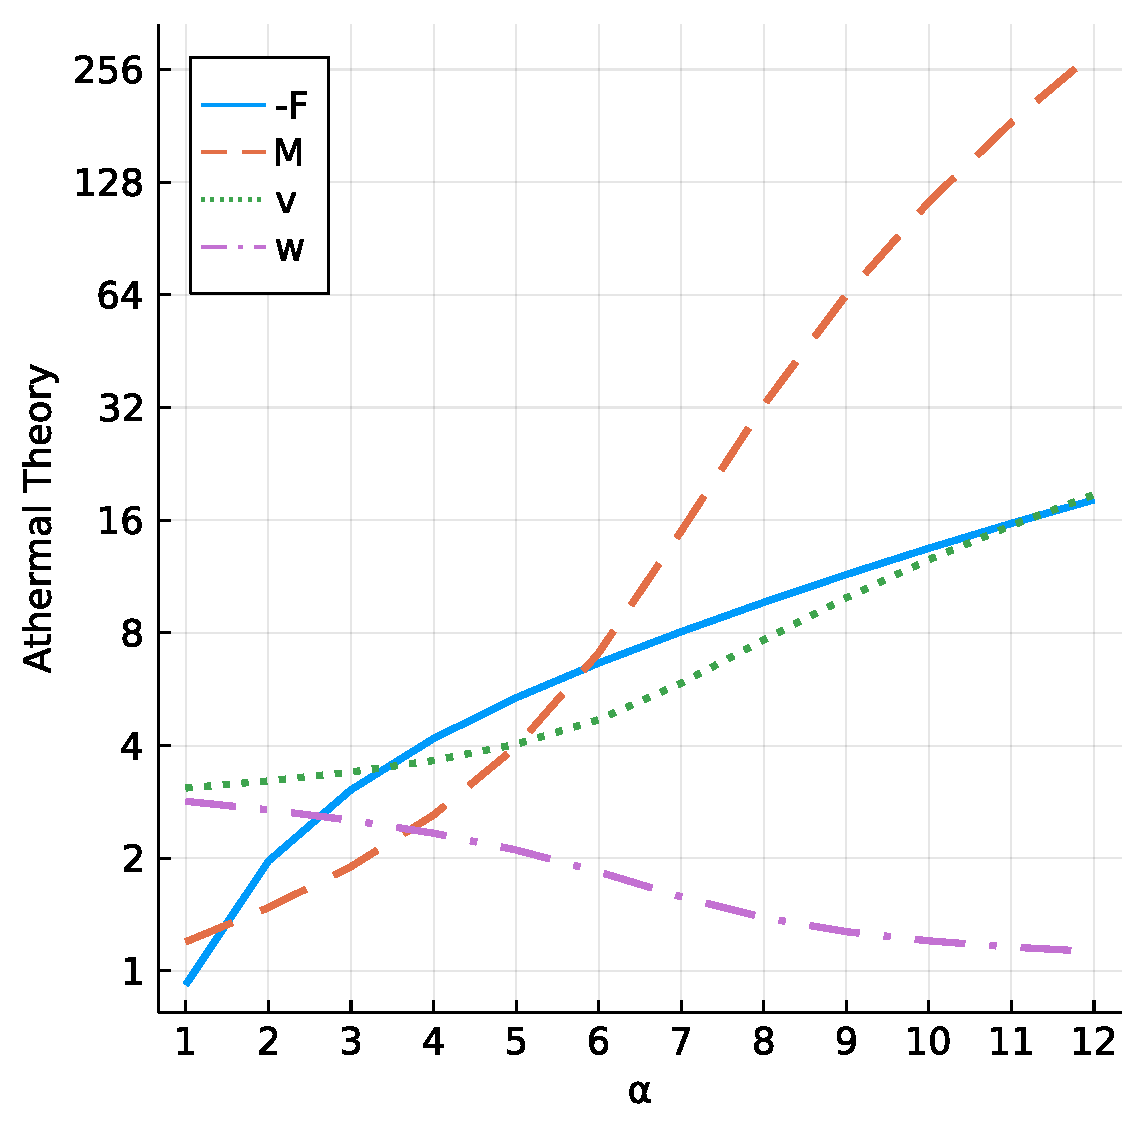
\includegraphics[width=.9\textwidth]{chapters/frohlich/figures/athermal_theory.pdf}
\end{subfigure}%
\begin{subfigure}[b]{.6\textwidth}
\centering
\includegraphics[width=.9\textwidth]{chapters/frohlich/figures/zero_temp_alpha.pdf}
\end{subfigure}%
}
\caption{(left): Unitless values from Feynman's athermal $0$K polaron theory, calculated for electron-phonon $\alpha$ couplings ranging from $1$ to $12$. Blue-solid is the negative of the best approximated ground-state energy $F$, orange-dashed is the polaron effective mass $m_b$, green-dotted is the $v$ variational parameter and purple-dash-dotted is the $w$ variational parameter. (right): The real conductivity (also the frequency-dependent mobility) of the polaron response obtained from the FHIP theory and calculated for $\alpha$ ranging from $1$ to $12$ and external field angular frequencies ranging from $0\ \omega_{LO}$ to $20\ \omega_{LO}$ multiples of the effective phonon angular frequency. The relative magnitudes of the curves for different values of $\alpha$ have been normalised and are not comparable.}
\label{fig:athermaltheory}
\end{figure}

Feynman's original path integral theory (\cite{feynman_slow_1955}) for the polaron produced a variational principle for the ground-state energy of the polaron. The variational $v$ and $w$ parameters that produce the best lower upper-bound to the ground-state energy are then used in expressions that Feynman derived for the polaron effective mass and complex conductivity. 

Figure \ref{fig:athermaltheory}a shows the values of the polaron ground-state energy $-E_{gs}$, effective mass $m_p$ and the corresponding $v$ and $w$, for values of the Fr\"ohlich $\alpha$ parameter ranging from $1$ to $12$. These data are all presented in their `polaron units' form for easier comparison to Feynman's original paper. The ground-state demonstrates the linear weak-coupling behaviour at smaller $\alpha$ before it becomes exponentially more negative as $\alpha$ increases (as the electron-phonon coupling strengthens). The effective mass starts as roughly equal to the conduction electron band-mass $m_p = m_b $ at small $\alpha$ and then becomes exponentially larger at stronger couplings. The $v$ and $w$ variational parameters start off as approximately equal with $v \approx w \approx 3$ at weak couplings, but diverge at strong couplings as $w$ asymptotically approaches $w = 1$ and $v$ increases exponentially at a similar rate to the ground-state energy. 

Figure \ref{fig:athermaltheory}b shows the athermal real conductivity (which is equivalent to the frequency-dependent polaron mobility) for $0 \leq \alpha \leq 12$ and for an applied electric field with an angular frequency $\Omega$ ranging from $0$ to $20$ times that of the longitudinal optical phonon frequency $\omega_{LO}$. At lower couplings $\alpha \leq 4$, all of the first peaks start at $\Omega = \omega_{LO}$ and for $\alpha \geq 5$ we see the appearance of additional peaks at $\Omega = \omega_{LO} + n \omega_{LO} v,\ n \in \mathbb{Z}^+$, with all of the peaks seemingly sharpening and blue-shifting to higher frequencies at stronger couplings $\alpha \geq 7$. However, for very strong couplings $\alpha \geq 10$ the initial peak at $\Omega = \omega_{LO}$ seems to appear again.

\subsection{Thermal theory}

Using \=Osaka's generalised variational principle, I was able to write codes that calculate the polaron free energy, effective mass and complex conductivity for temperatures $T$ ranging from $1$ to $10$ multiples of $\omega_{LO}$ (here $\hbar = k_B = 1$) and for $1\leq\alpha\leq12$. 

In Figure \ref{fig:thermaltheory} are contour plots that show, as a function of temperature $T / \omega_{LO}$ and $\alpha$, (a) the polaron free energy, (b) the polaron effective mass, (c) values of the $v$ variational parameters and (d) values of the $w$ variational parameter. The free energy shows similar behaviour at low temperatures $T \gtrsim \hbar \omega_{LO} / k_B$ to the ground-state energy, but then seems to shift more negative with an increasing negative gradient for $T \gtrsim \hbar \omega_{LO} / k_B$. The effective mass follows a similar pattern as it has a roughly the same behaviour for $T \lesssim \hbar \omega_{LO} / k_B$ as it did for $T = 0$, but becomes exponentially more positive for temperatures $T \gtrsim \hbar \omega_{LO} / k_B$. The $v$ and $w$ parameters also show this pattern and increase exponentially with temperature beyond $T \gtrsim \hbar \omega_{LO} / k_B$. However, $v$ grows faster than $w$ so their difference increases exponentially with temperature too. The artefacts that appear in contour plots for the effective mass and variational parameters at lower $\alpha$ and high temperatures may be numerical error due to difficulties in the optimisation process. The free energy seems to vary less with temperature at weak coupling which may have made finding the global minima difficult, resulting in noise. 

Figure \ref{fig:dcmobility} shows a contour plot of the dc mobility derived in FHIP (note that this expression is unitless). For temperatures $T \lesssim \hbar \omega_{LO} / 2 k_B$ the dc mobility has a minimum around $\alpha \approx 7$ which shifts to larger values of $\alpha$ as the temperature increases. Similarly, for $\alpha \geq 7$ the mobility seems to be minimum around temperatures $T \approx \hbar \omega_{LO} / k_B$. Elsewhere, for $\alpha < 7$ the mobility seems to decrease rapidly as the temperature increases from $0$K up until $T \approx \hbar \omega_{LO} / k_B$, then above this temperature it decreases asymptotically towards zero.

\begin{figure}
\vspace*{-1.5cm}\makebox[\linewidth][c]{%
\begin{subfigure}[t]{0.01\textwidth}
    \vspace*{-7.5cm}\textbf{a}
  \end{subfigure}%
\begin{subfigure}[b]{.6\textwidth}
\centering
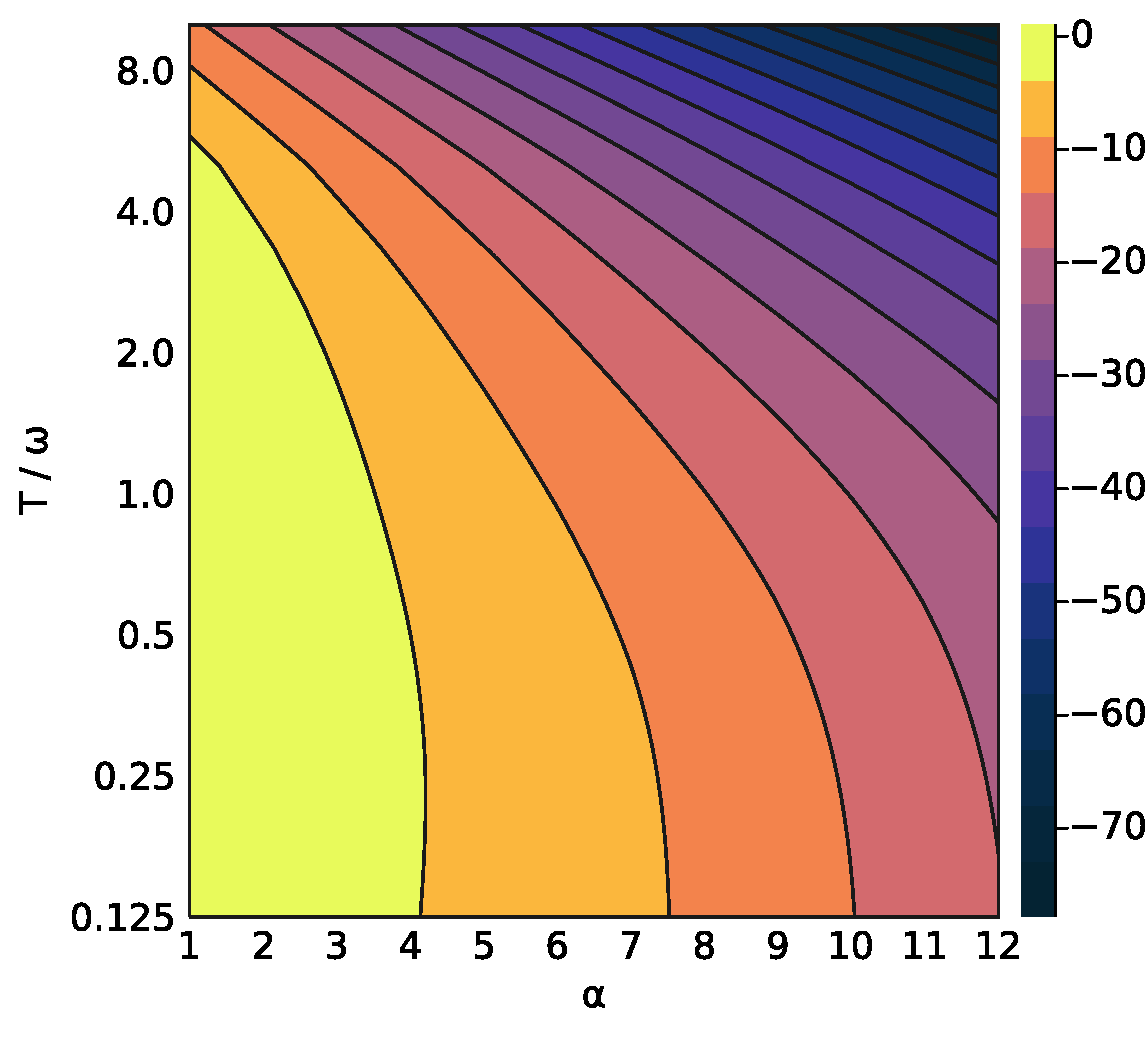
\includegraphics[width=.95\textwidth]{chapters/frohlich/figures/free_energy.pdf}
\end{subfigure}%
\begin{subfigure}[t]{0.01\textwidth}
    \vspace*{-7.5cm}\textbf{b}
  \end{subfigure}
\begin{subfigure}[b]{.6\textwidth}
\centering
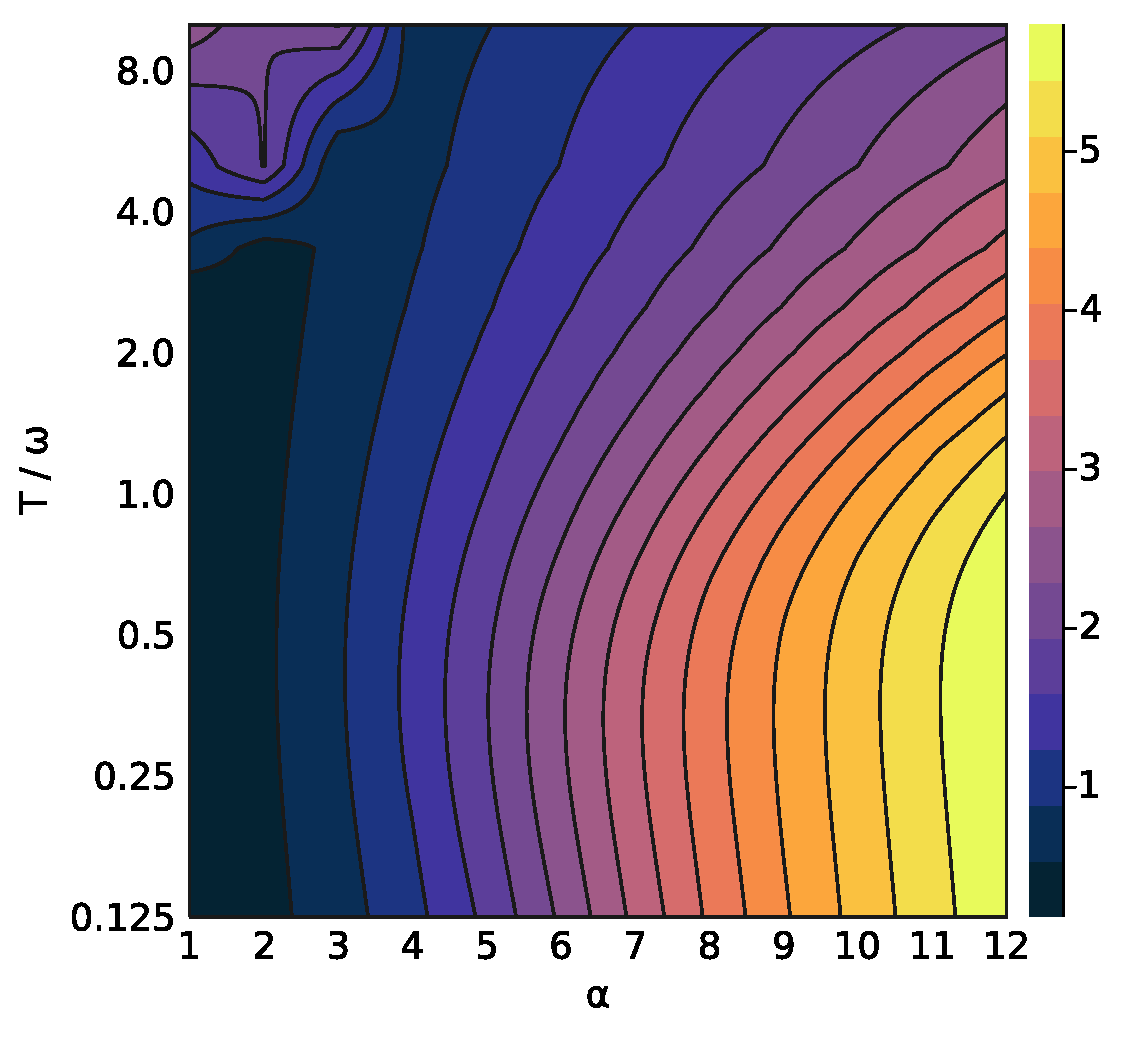
\includegraphics[width=.95\textwidth]{chapters/frohlich/figures/effective_mass.pdf}
\end{subfigure}%
}\\
\makebox[\linewidth][c]{%
\begin{subfigure}[t]{0.01\textwidth}
    \vspace*{-7.5cm}\textbf{c}
  \end{subfigure}%
\begin{subfigure}[b]{.6\textwidth}
\centering
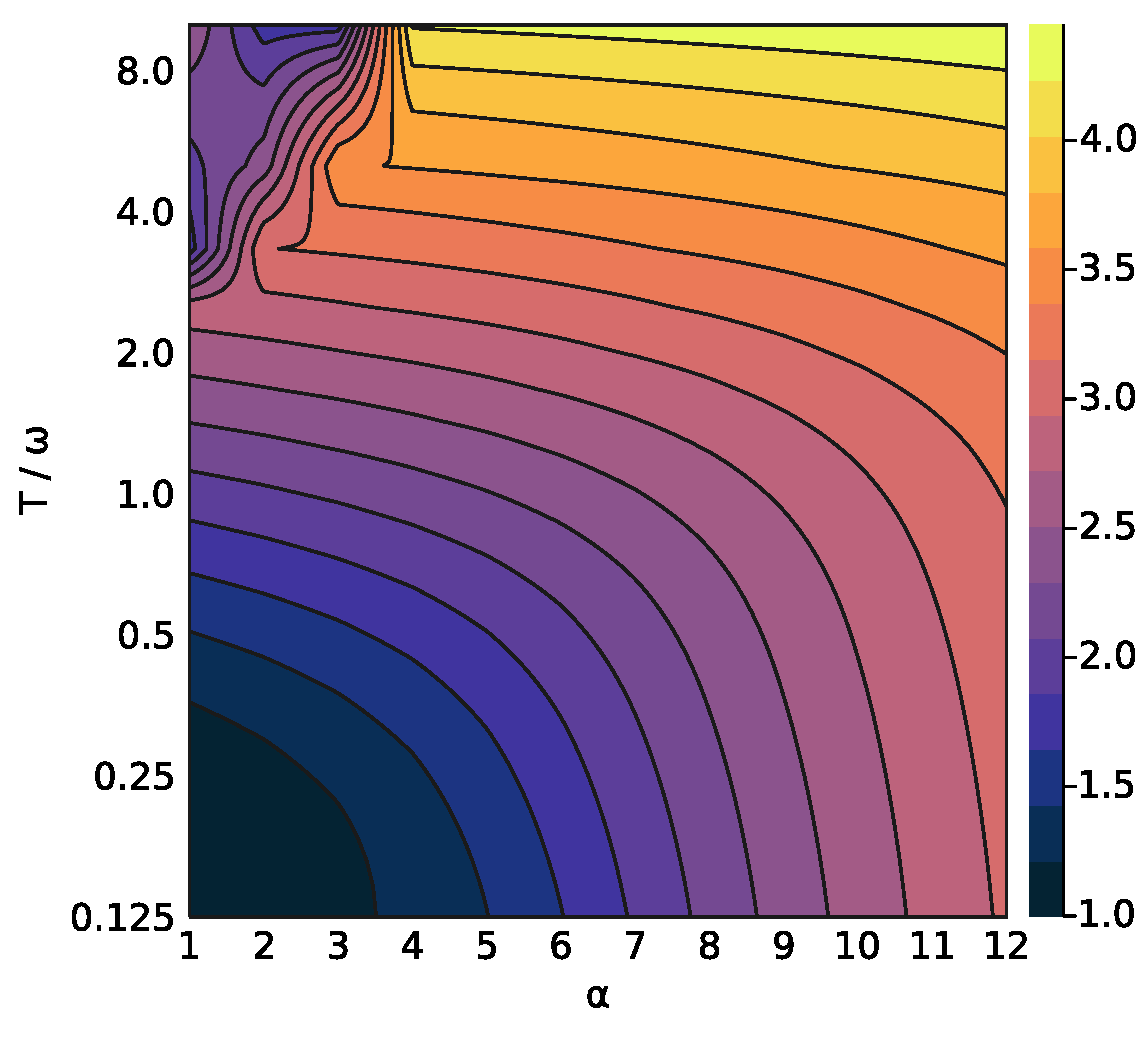
\includegraphics[width=.95\textwidth]{chapters/frohlich/figures/v_parameter.pdf}
\end{subfigure}%
\begin{subfigure}[t]{0.01\textwidth}
    \vspace*{-7.5cm}\textbf{d}
  \end{subfigure}%
\begin{subfigure}[b]{.6\textwidth}
\centering
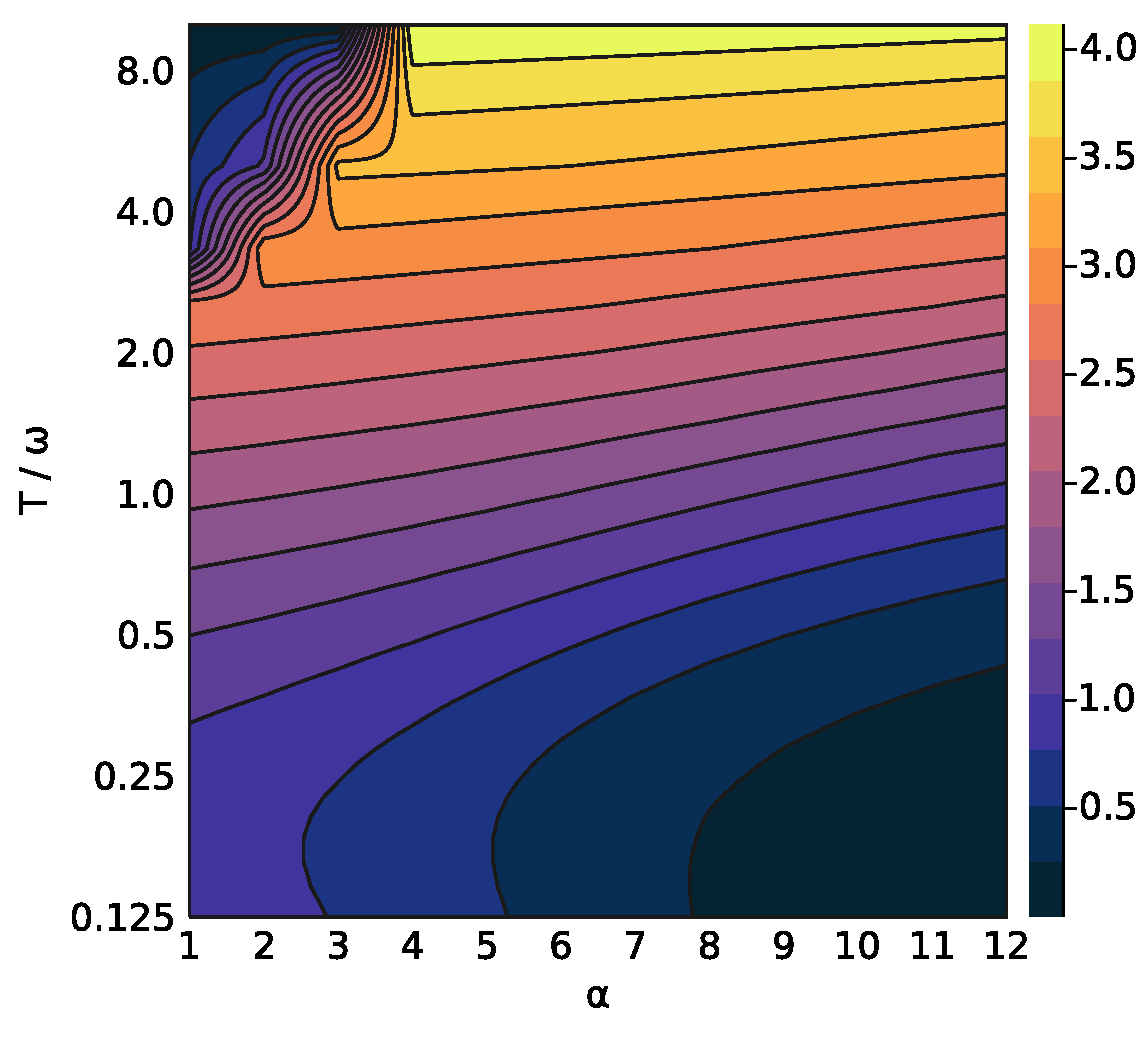
\includegraphics[width=.95\textwidth]{chapters/frohlich/figures/w_parameter.pdf}
\end{subfigure}%
}
\caption{Contour plots of (a) \=Osaka's polaron free energy, (b) Feynman's effective mass (log scale), (c) the $v$ variational parameter (log scale) and (d) the $w$ varational parameter (log scale), as a function of `effective' temperature $T / \omega_{LO}$ and the Fr\"ohlich $\alpha$ parameter.}
\label{fig:thermaltheory}
\end{figure}

\subsection{Optical absorption and complex conductivity}

\begin{figure}
\vspace*{-1.6cm}
\makebox[\linewidth][c]{%
\begin{subfigure}[b]{.65\textwidth}
\centering
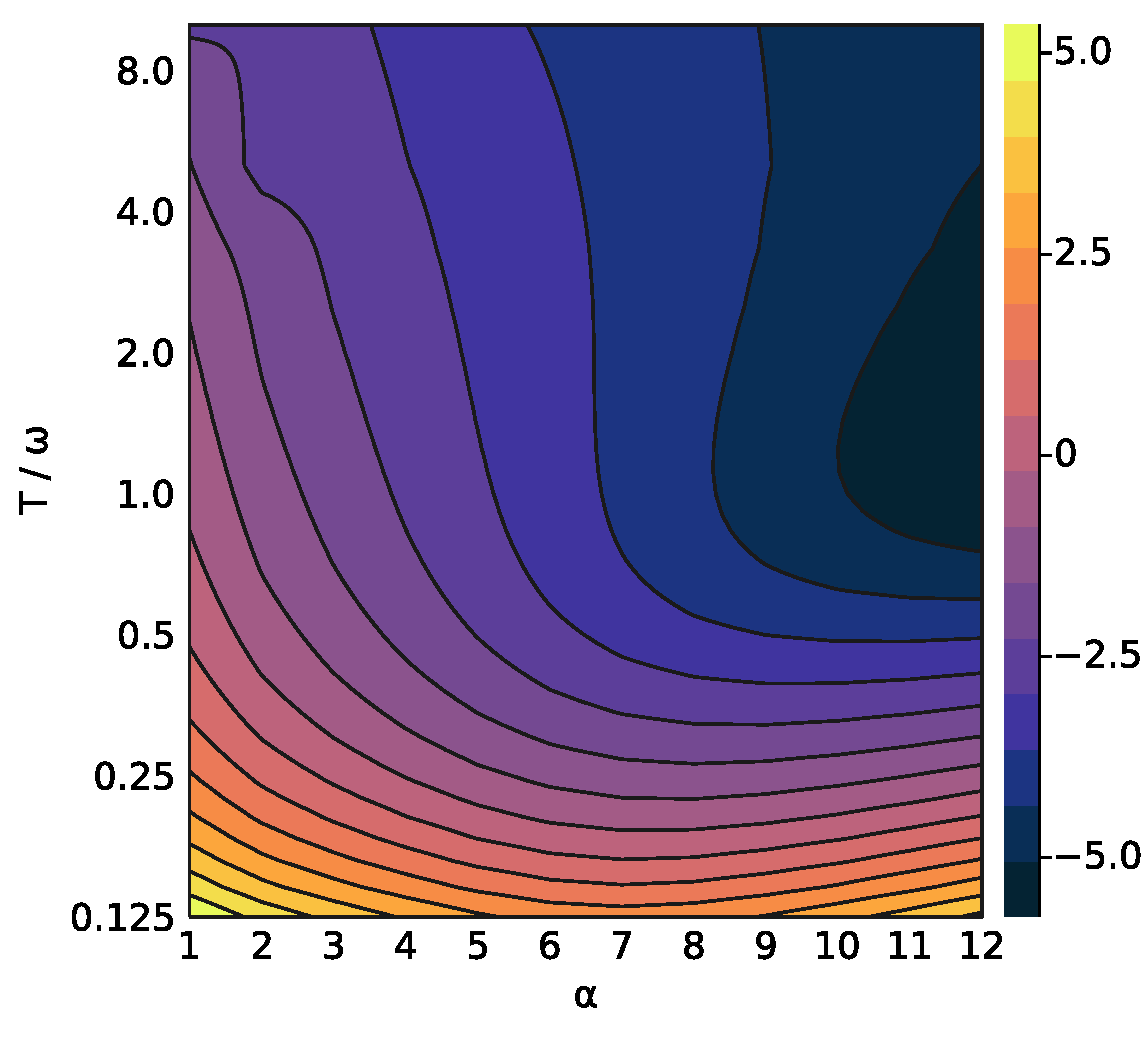
\includegraphics[width=1\textwidth]{chapters/frohlich/figures/dc_mobility.pdf}
\end{subfigure}
}
\caption{Log contour plot of the dc mobility (arbitrary units).}
\label{fig:dcmobility}
\end{figure}

I used the optical absorption expression obtained from~\cite{devreese_optical_1972} to extend the codes to calculate the complex conductivity of the polaron for different couplings $1 \leq \alpha \leq 12$, temperatures $0 \leq T / \omega_{LO} \leq 10$ and applied electric field frequencies $0 \leq \Omega / \omega_{LO} \leq 20$. I show the data obtained for $\alpha = 3, 6, 9$ where perturbation theory breaks down at $\alpha = 6$. 

Figures \ref{fig:osakacontour} (contour plots) and \ref{fig:osakaridge} (ridge-line plots) show the real (left columns) and imaginary (right columns) of the complex conductivity for $\alpha = 3$ in the first rows, $\alpha = 6$ in the second rows and $\alpha = 9$ in the last rows. The figures are all log-scaled with respect to the complex conductivity, and for the imaginary component I have taken the absolute value in order to go to the log-scale. This means that for the imaginary plots, any sharp `rifts' indicate a change in sign as the imaginary component passes through zero. The imaginary component always starts negative at low temperature and frequency, so the first rift can be assumed to indicate a change to a positive sign and so on. I chose $\alpha = 3, 6, 9$ to give some spread of coupling strength about $\alpha = 6$ where perturbation theory typically breaks down. 

From Figures \ref{fig:osakacontour} and \ref{fig:osakaridge} we can see that firstly, at $\alpha = 3$ the complex conductivity starts with a single peak starting at $\Omega = \omega_{LO}$ for zero temperature, which broadens out and blue-shifts to higher frequencies as the temperature increases. This peak corresponds to a single phonon excitation. At $\alpha = 6$ the conductivity develops more peaks starting at $\Omega = \omega_{LO} + n \omega_{LO} v,\ n \in \mathbb{Z}^+$ at zero temperature, corresponding to further phonon excitations, which also broaden out and blue-shift to higher frequencies as the temperature increases. The first peak for $\alpha = 6$ now has more features, with an initial shoulder which leads into a far sharper peak than before, and sharper, more structured peaks as $\alpha$ increases. Finally, for $\alpha = 9$ the landscape becomes much more erratic and complex. The first peak still remains, however the trough that follows it has become so deep (reaching values close to zero) that the numerical results is noisy due to reaching float-point accuracy (working here with 64-bit floats). The second main peak (that I identify as regions now separated by the deep troughs) now seems to begin a little earlier than $\Omega = \omega_{LO} + v \omega_{LO}$ and appears to be composed of smaller, sharper peaks and shoulders. 

\begin{figure}[h]
\vspace*{-1.5cm}\makebox[\linewidth][c]{%
\begin{subfigure}[t]{0.01\textwidth}
    \vspace*{-8.2cm}\hspace*{9.4cm}\textbf{$\vb{\alpha}$=3}
    \vspace*{-7.5cm}\textbf{a}
  \end{subfigure}%
\begin{subfigure}[b]{.6\textwidth}
\centering
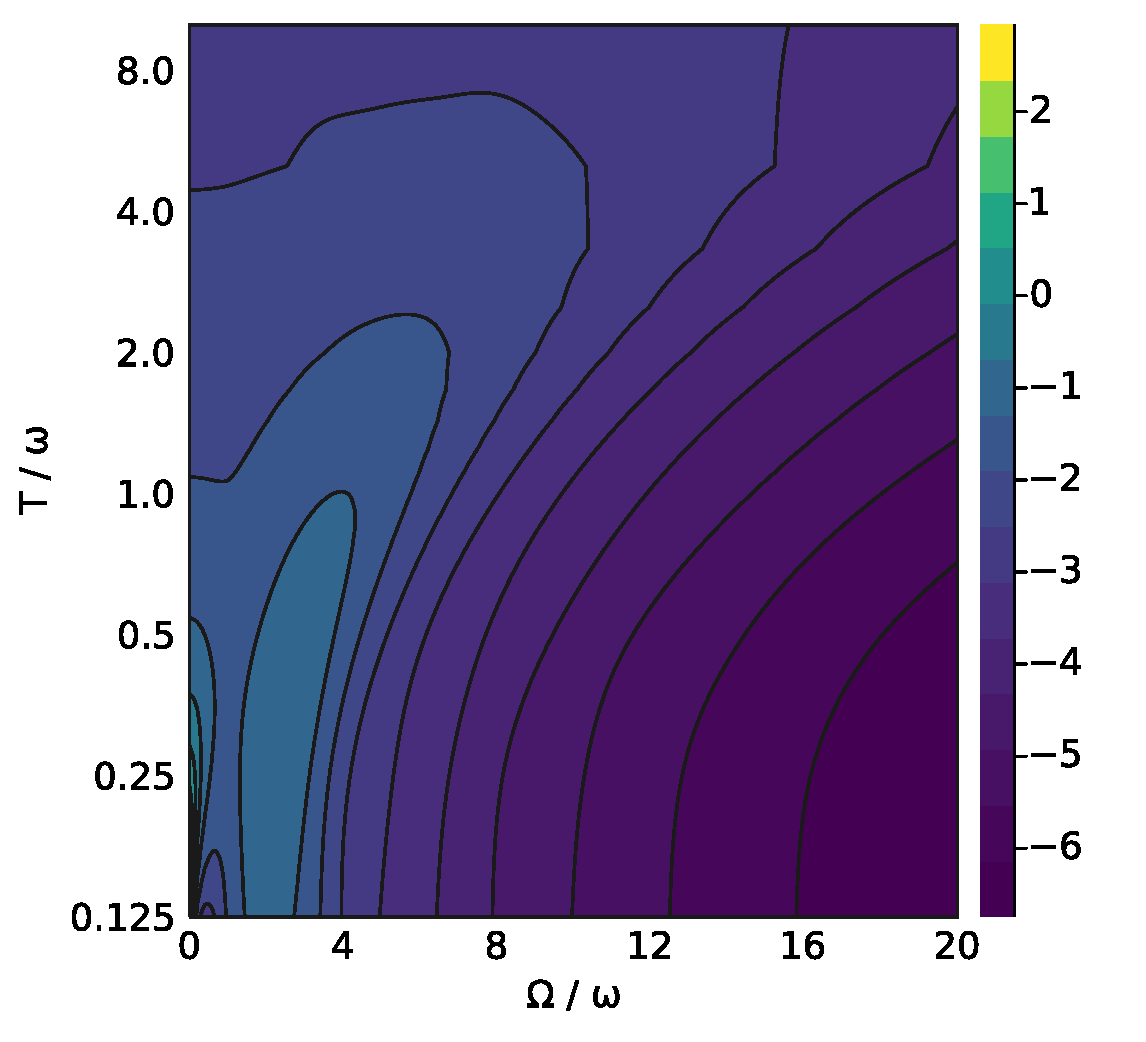
\includegraphics[width=.92\textwidth]{chapters/frohlich/figures/conductivity_contour_real_3.pdf}
\end{subfigure}%
\begin{subfigure}[t]{0.01\textwidth}
    \vspace*{-7.5cm}\textbf{b}
  \end{subfigure}
\begin{subfigure}[b]{.6\textwidth}
\centering
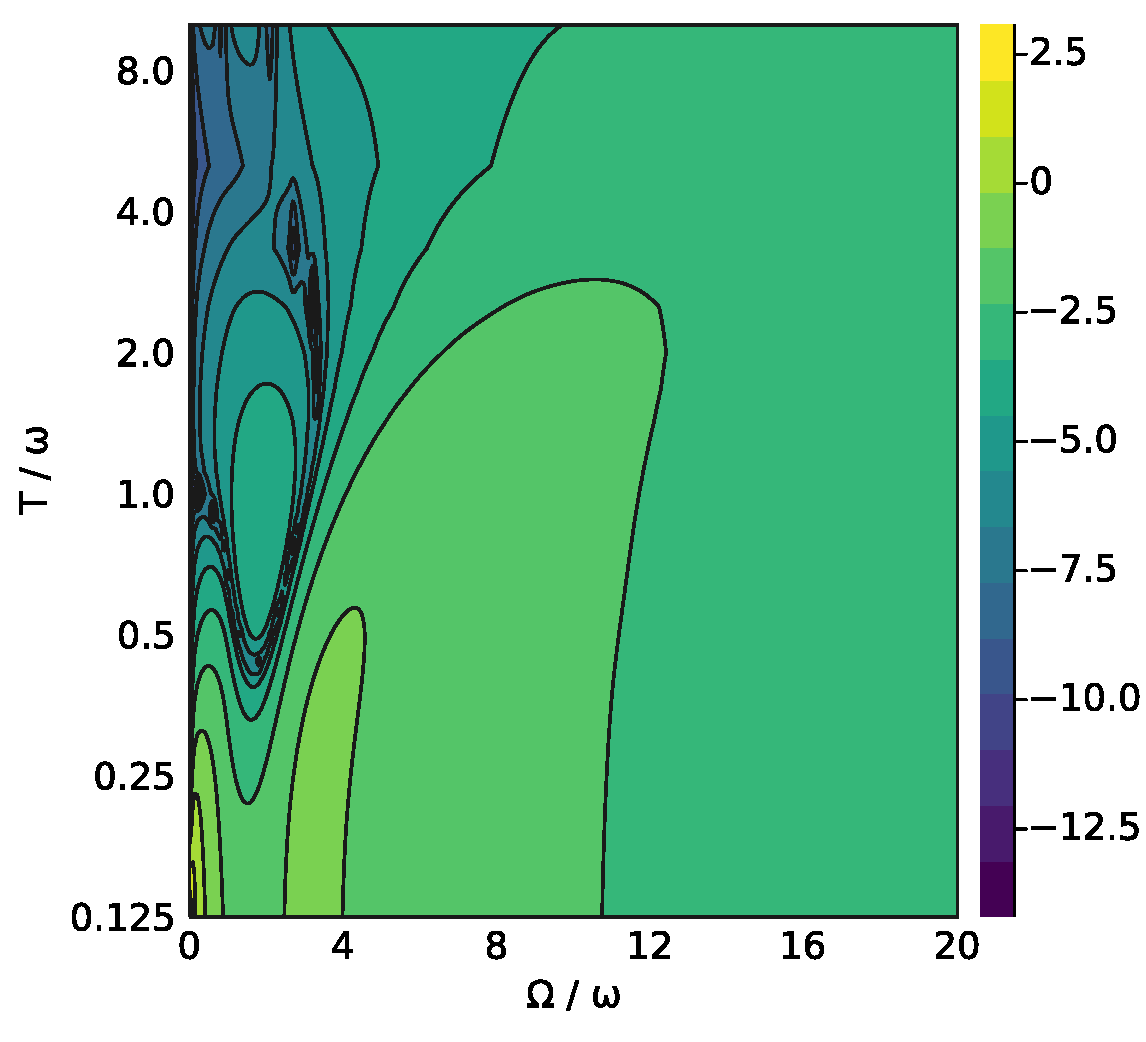
\includegraphics[width=.92\textwidth]{chapters/frohlich/figures/conductivity_contour_imag_3.pdf}
\end{subfigure}%
}\\
\makebox[\linewidth][c]{%
\begin{subfigure}[t]{0.01\textwidth}
    \vspace*{-8.2cm}\hspace*{9.4cm}\textbf{$\vb{\alpha}$=6}
    \vspace*{-7.5cm}\textbf{c}
  \end{subfigure}%
\begin{subfigure}[b]{.6\textwidth}
\centering
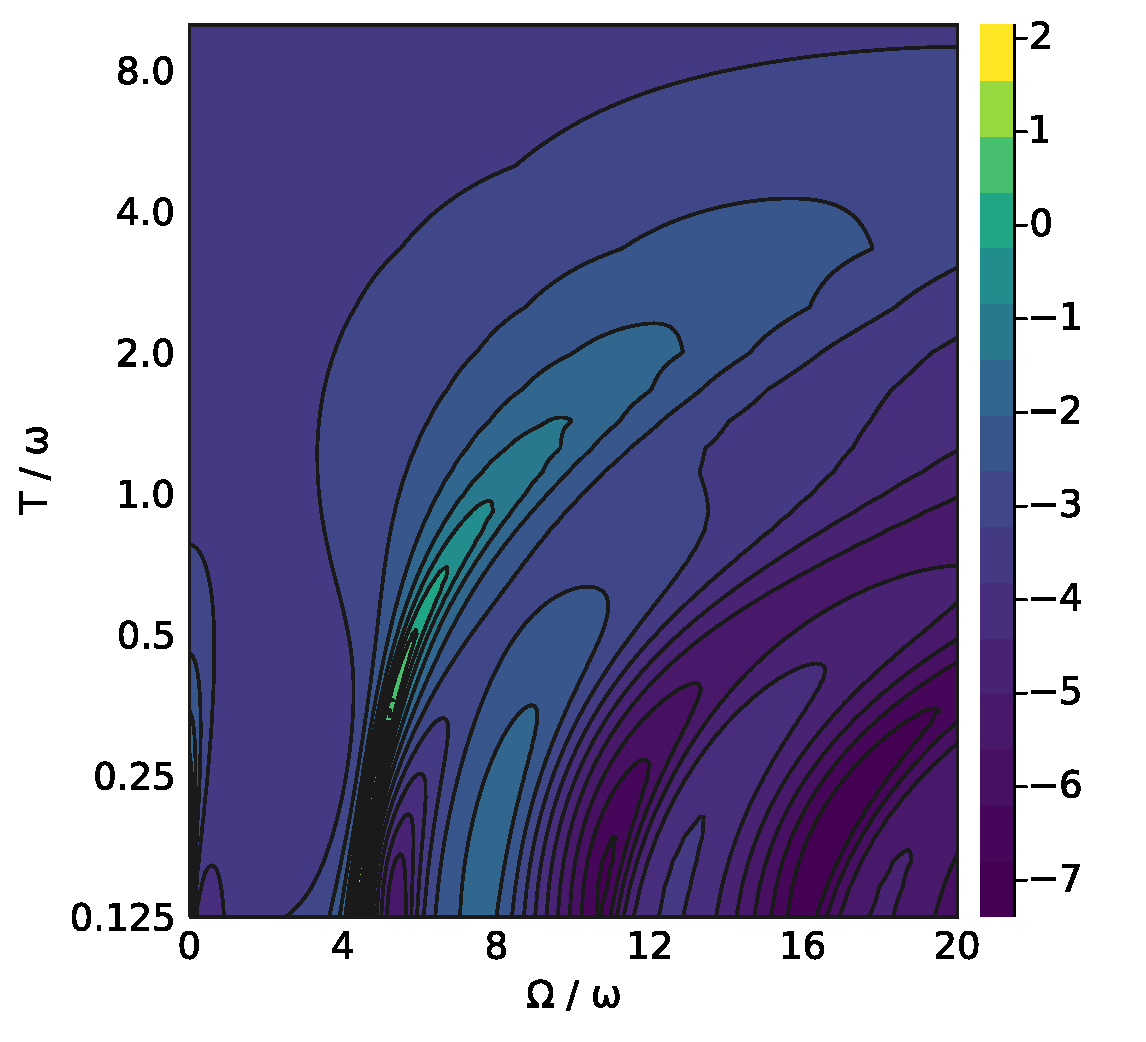
\includegraphics[width=.92\textwidth]{chapters/frohlich/figures/conductivity_contour_real_6.pdf}
\end{subfigure}%
\begin{subfigure}[t]{0.01\textwidth}
    \vspace*{-7.5cm}\textbf{d}
  \end{subfigure}%
\begin{subfigure}[b]{.6\textwidth}
\centering
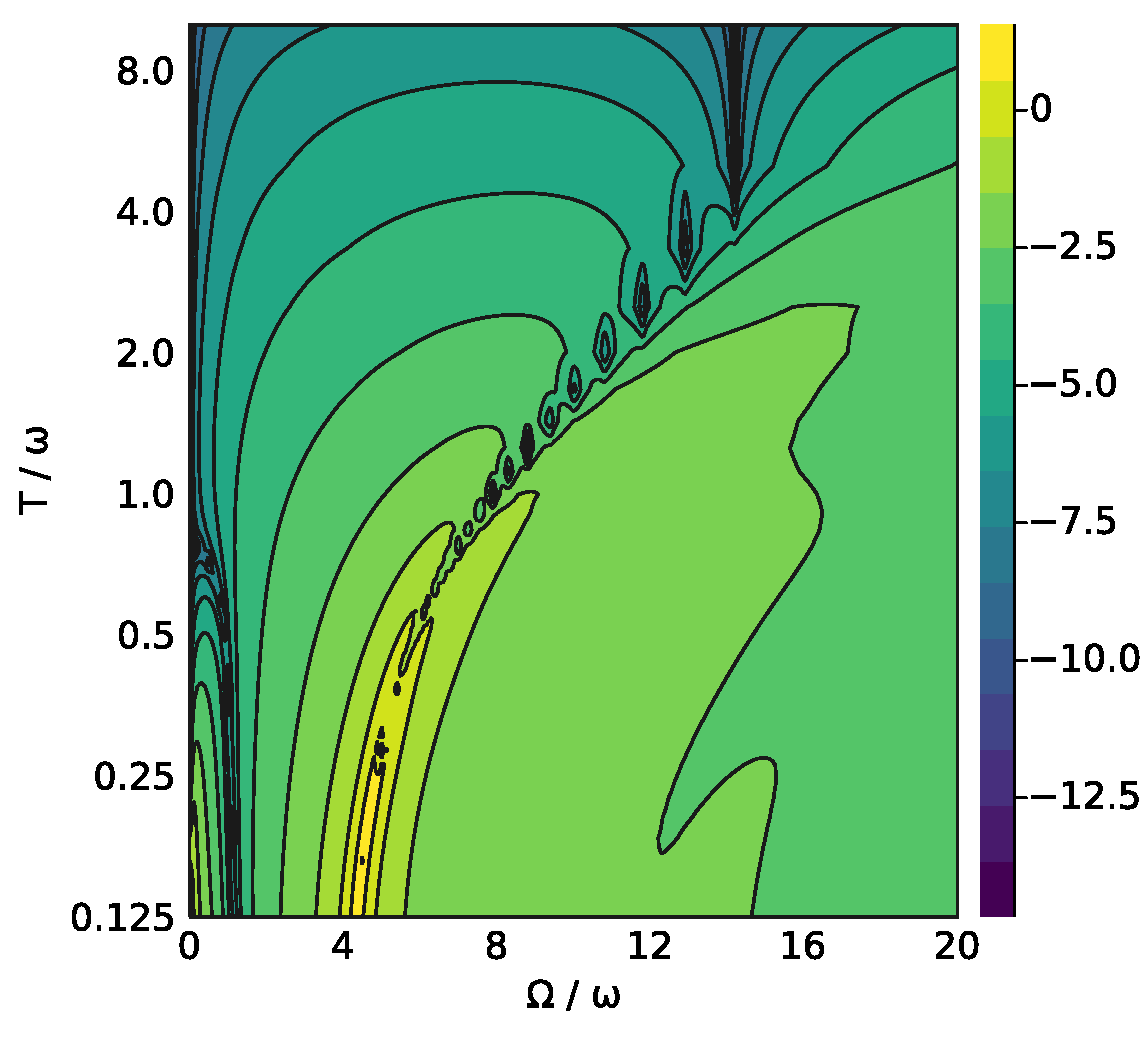
\includegraphics[width=.92\textwidth]{chapters/frohlich/figures/conductivity_contour_imag_6.pdf}
\end{subfigure}%
}
\makebox[\linewidth][c]{%
\begin{subfigure}[t]{0.01\textwidth}
    \vspace*{-8.2cm}\hspace*{9.4cm}\textbf{$\vb{\alpha}$=9}
    \vspace*{-7.5cm}\textbf{e}
  \end{subfigure}%
\begin{subfigure}[b]{.6\textwidth}
\centering
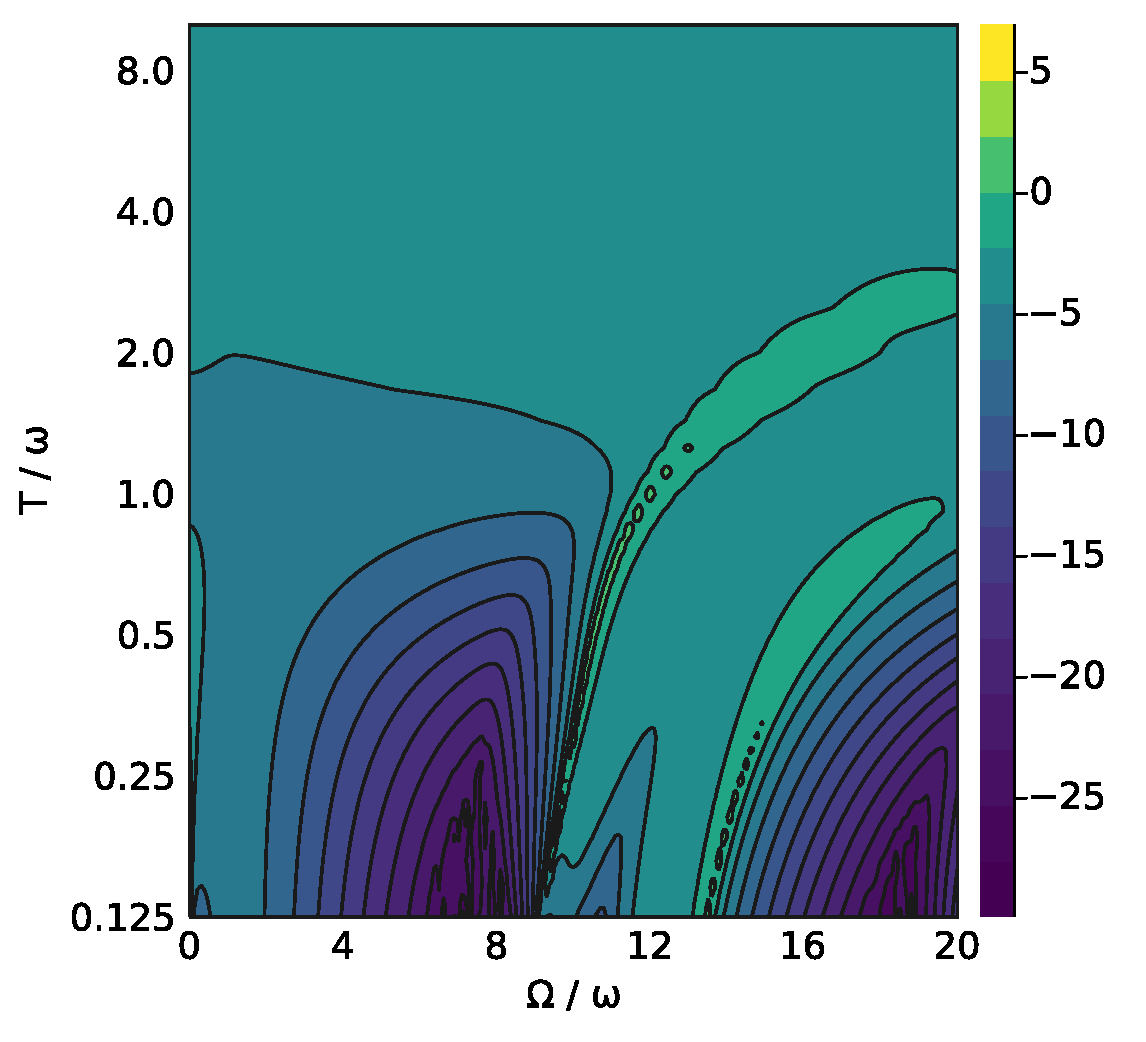
\includegraphics[width=.92\textwidth]{chapters/frohlich/figures/conductivity_contour_real_9.pdf}
\end{subfigure}%
\begin{subfigure}[t]{0.01\textwidth}
    \vspace*{-7.5cm}\textbf{f}
  \end{subfigure}%
\begin{subfigure}[b]{.6\textwidth}
\centering
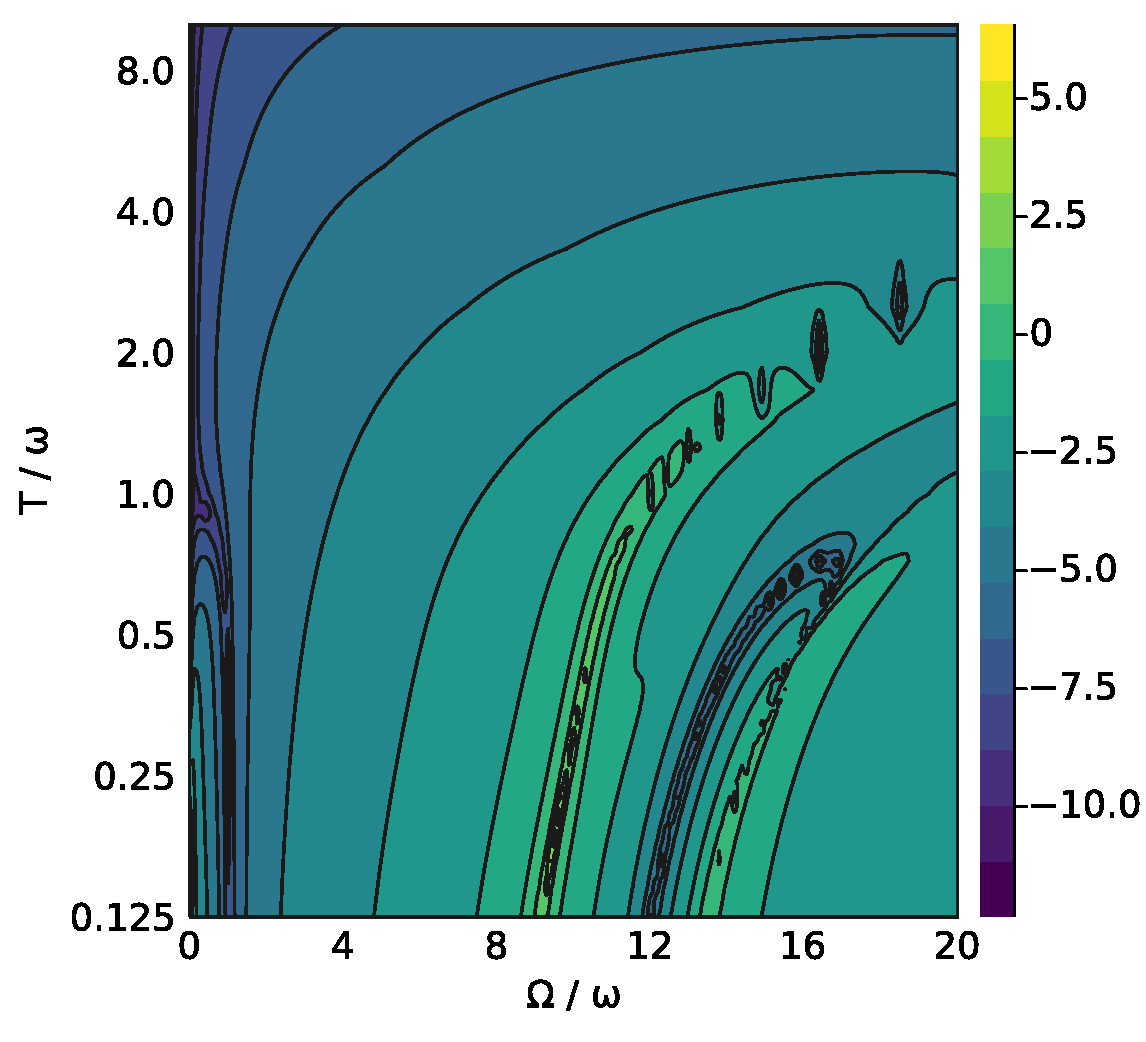
\includegraphics[width=.92\textwidth]{chapters/frohlich/figures/conductivity_contour_imag_9.pdf}
\end{subfigure}%
}
\caption{Contours for the real (left) and imaginary (right) complex conductivity at different values of $\alpha$. (a) Real conductivity at $\alpha = 3$. (b) Imaginary conductivity at $\alpha = 3$. (c) Real conductivity at $\alpha = 6$. (d) Imaginary conductivity at $\alpha = 6$. (e) Real conductivity at $\alpha = 9$. (f) Imaginary conductivity at $\alpha = 9$.}
\label{fig:osakacontour}
\end{figure}

\begin{figure}[h]
\vspace*{-1.5cm}\makebox[\linewidth][c]{%
\begin{subfigure}[t]{0.01\textwidth}
    \vspace*{-8.2cm}\hspace*{9.2cm}\textbf{\underline{$\vb{\alpha}$=3}}
    \vspace*{-7.5cm}\textbf{a}
  \end{subfigure}%
\begin{subfigure}[b]{.58\textwidth}
\centering
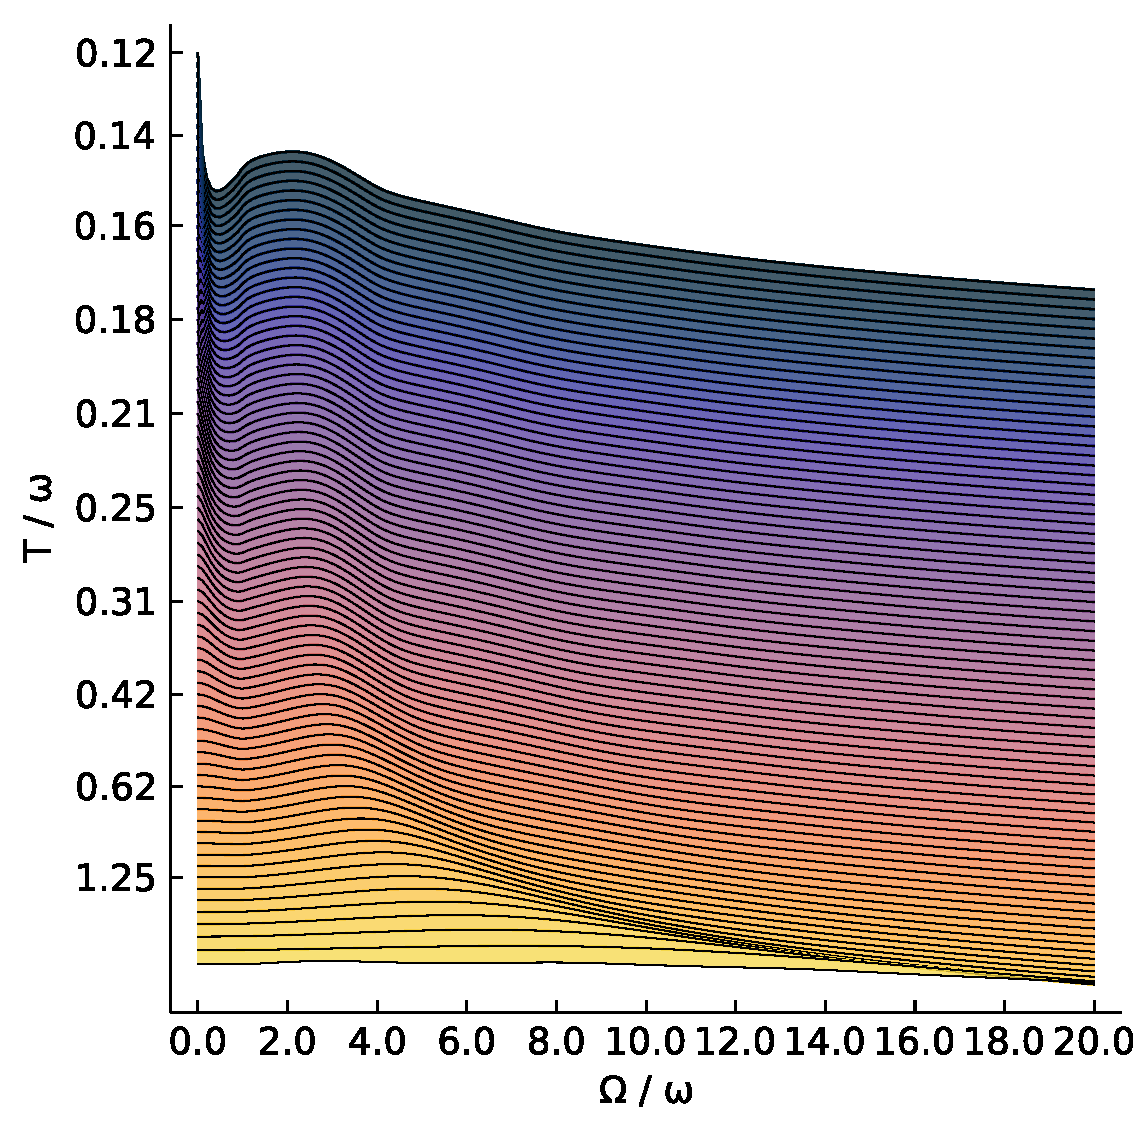
\includegraphics[width=.87\textwidth]{chapters/frohlich/figures/conductivity_plot_temp_real_3.pdf}
\end{subfigure}%
\begin{subfigure}[t]{0.01\textwidth}
    \vspace*{-7.5cm}\textbf{b}
  \end{subfigure}
\begin{subfigure}[b]{.58\textwidth}
\centering
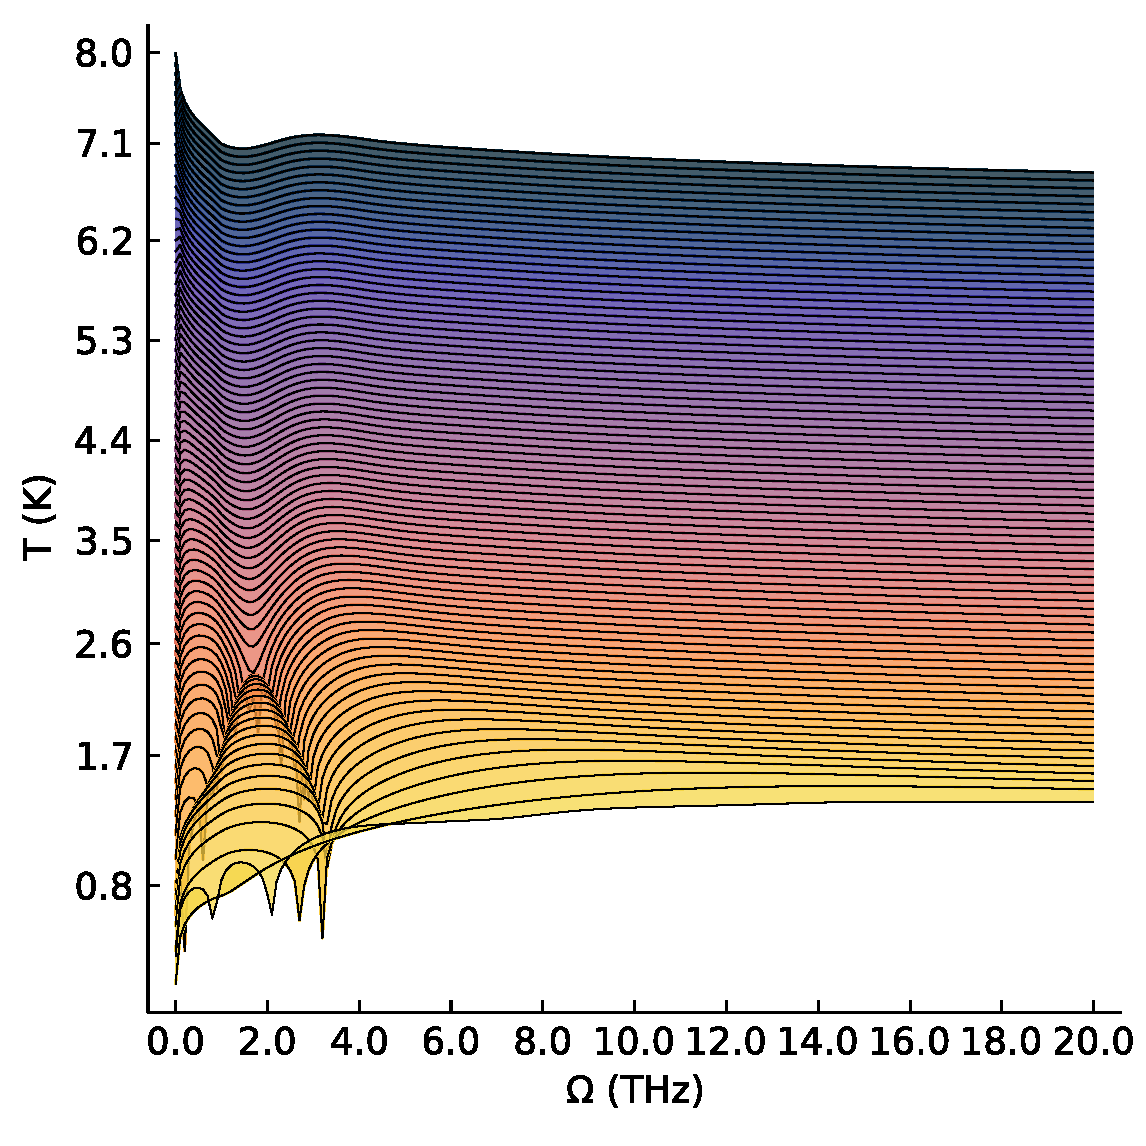
\includegraphics[width=.87\textwidth]{chapters/frohlich/figures/conductivity_plot_temp_imag_3.pdf}
\end{subfigure}%
}\\
\makebox[\linewidth][c]{%
\begin{subfigure}[t]{0.01\textwidth}
    \vspace*{-8.2cm}\hspace*{9.2cm}\textbf{\underline{$\vb{\alpha}$=6}}
    \vspace*{-7.5cm}\textbf{c}
  \end{subfigure}%
\begin{subfigure}[b]{.58\textwidth}
\centering
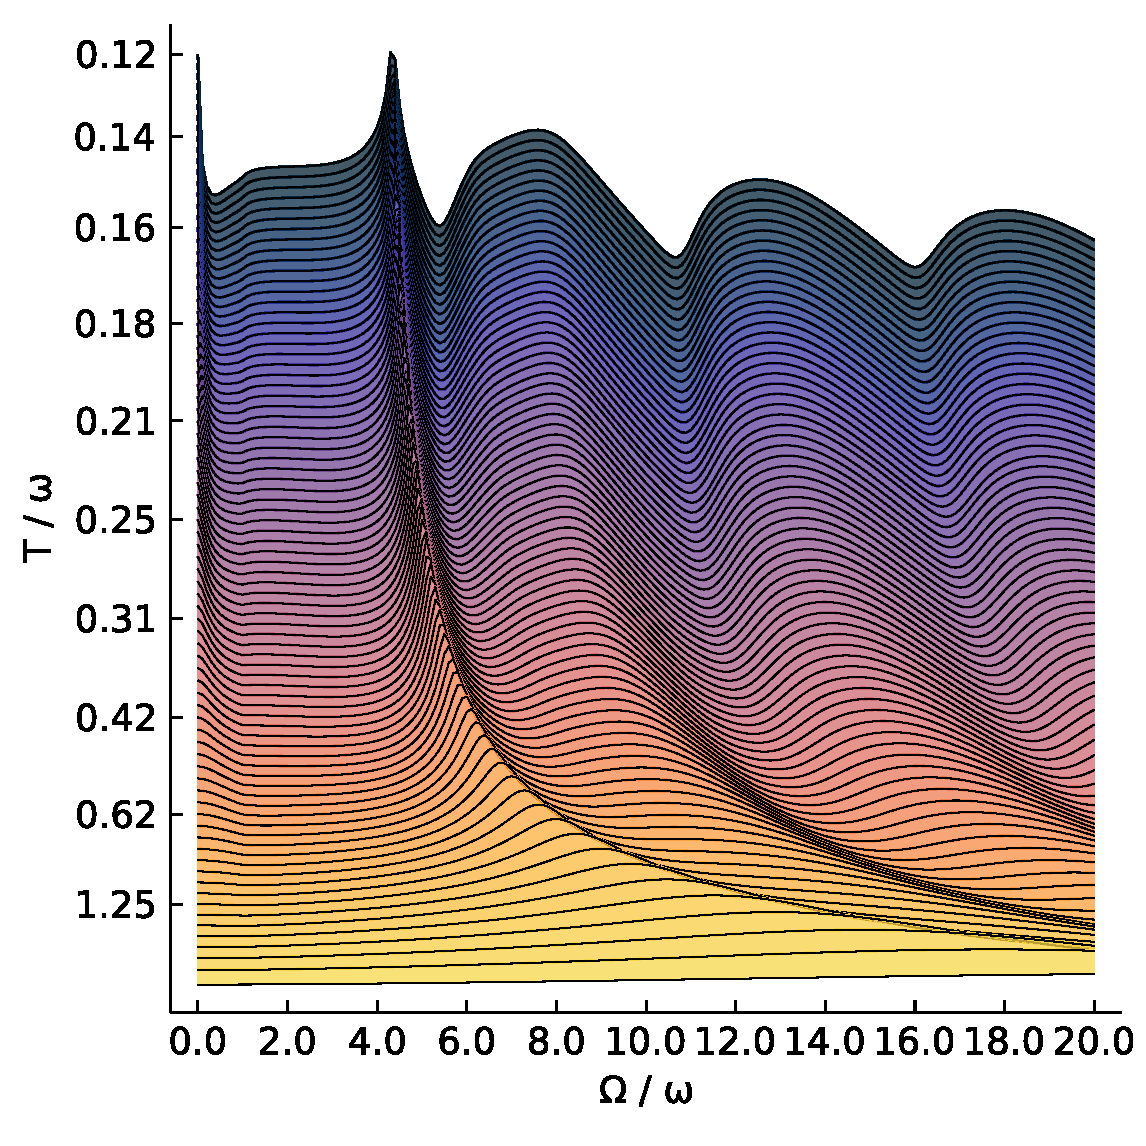
\includegraphics[width=.87\textwidth]{chapters/frohlich/figures/conductivity_plot_temp_real_6.pdf}
\end{subfigure}%
\begin{subfigure}[t]{0.01\textwidth}
    \vspace*{-7.5cm}\textbf{d}
  \end{subfigure}%
\begin{subfigure}[b]{.58\textwidth}
\centering
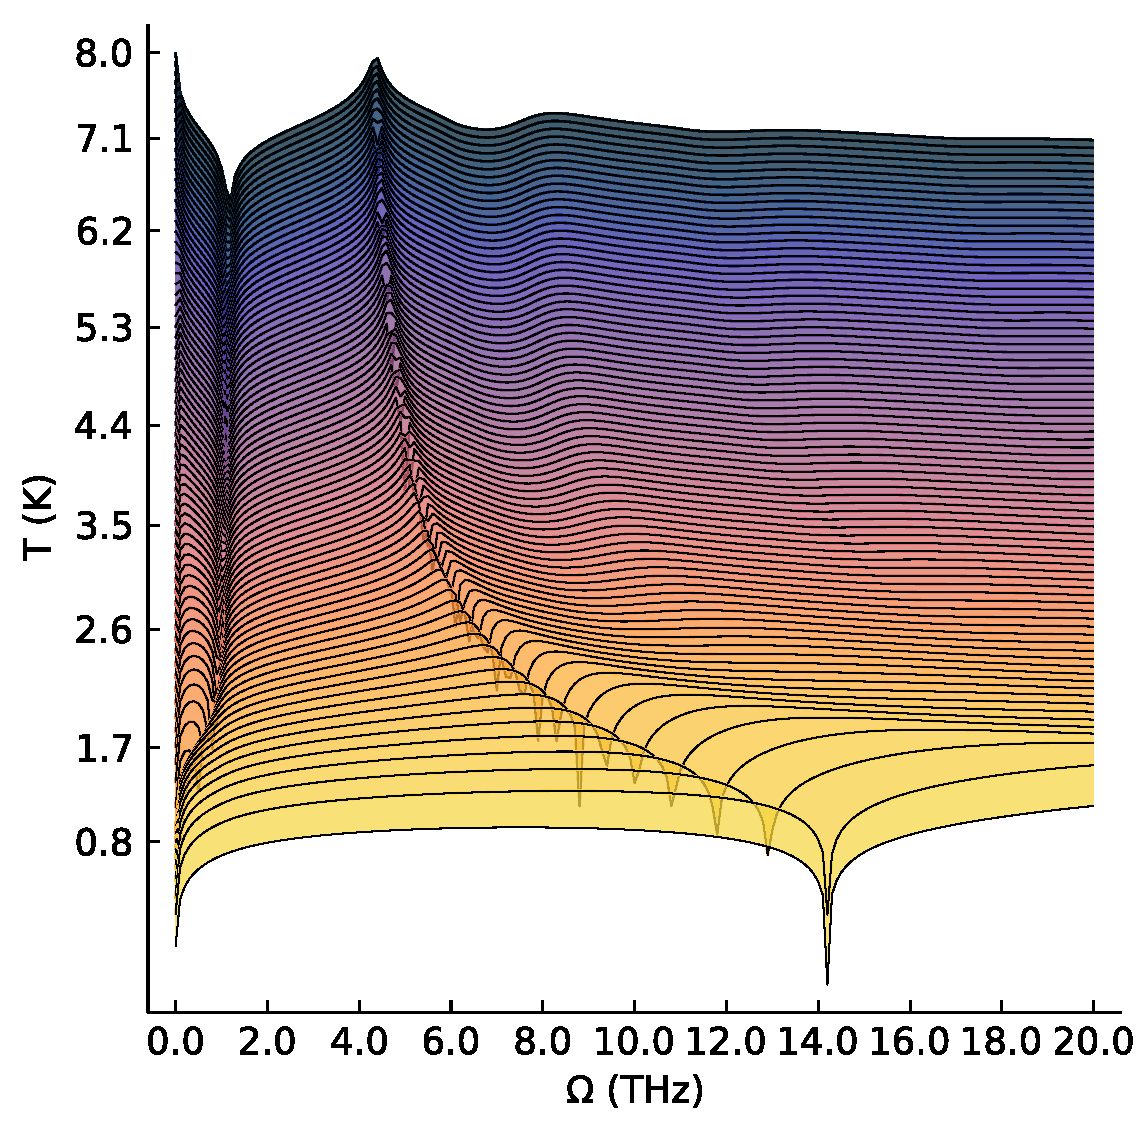
\includegraphics[width=.87\textwidth]{chapters/frohlich/figures/conductivity_plot_temp_imag_6.pdf}
\end{subfigure}%
}
\makebox[\linewidth][c]{%
\begin{subfigure}[t]{0.01\textwidth}
    \vspace*{-8.2cm}\hspace*{9.2cm}\textbf{\underline{$\vb{\alpha}$=9}}
    \vspace*{-7.5cm}\textbf{e}
  \end{subfigure}%
\begin{subfigure}[b]{.58\textwidth}
\centering
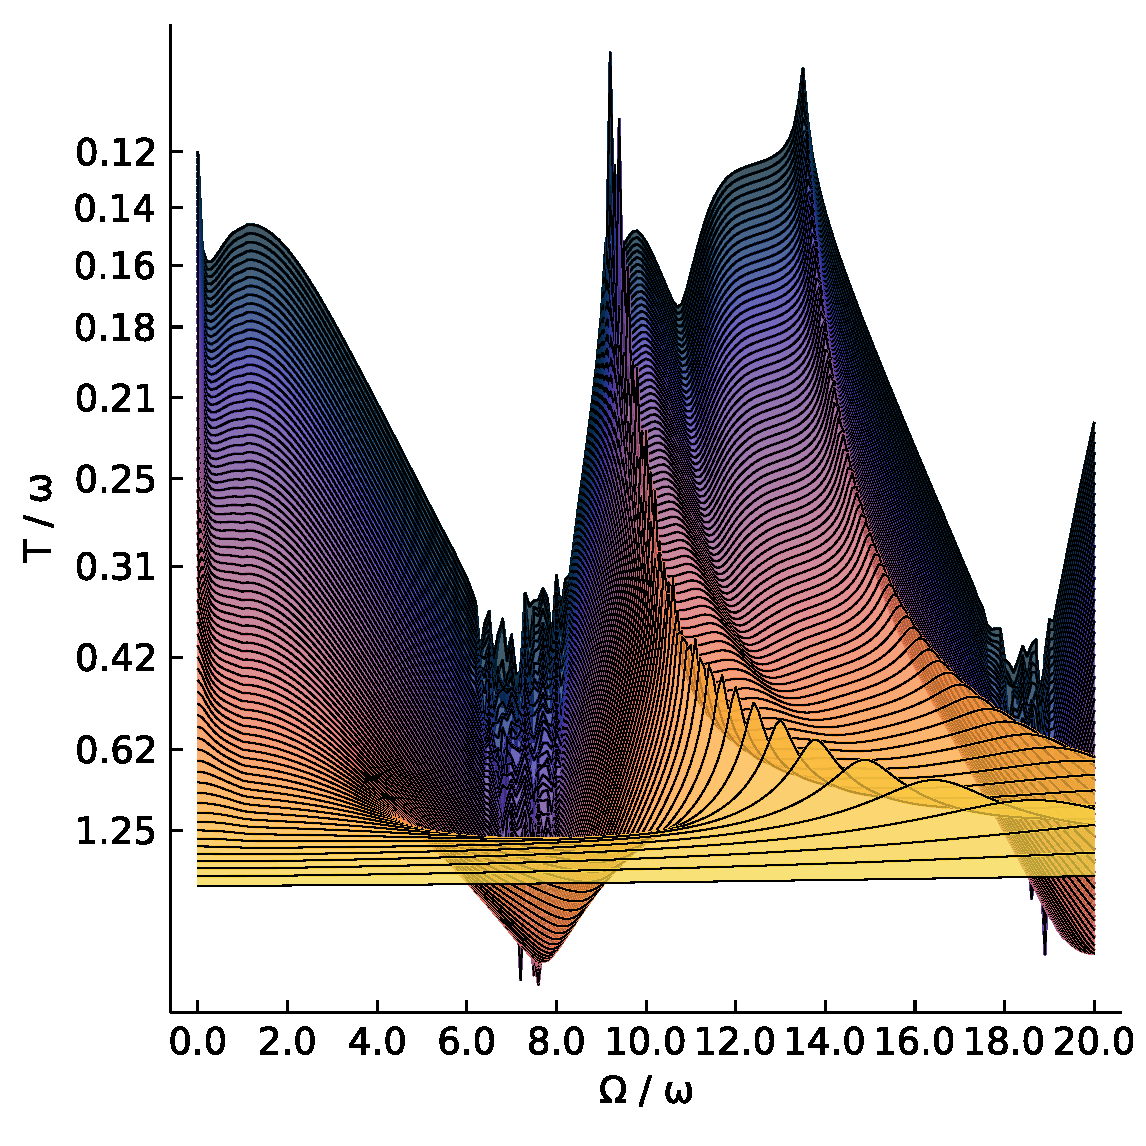
\includegraphics[width=.87\textwidth]{chapters/frohlich/figures/conductivity_plot_temp_real_9.pdf}
\end{subfigure}%
\begin{subfigure}[t]{0.01\textwidth}
    \vspace*{-7.5cm}\textbf{f}
  \end{subfigure}%
\begin{subfigure}[b]{.58\textwidth}
\centering
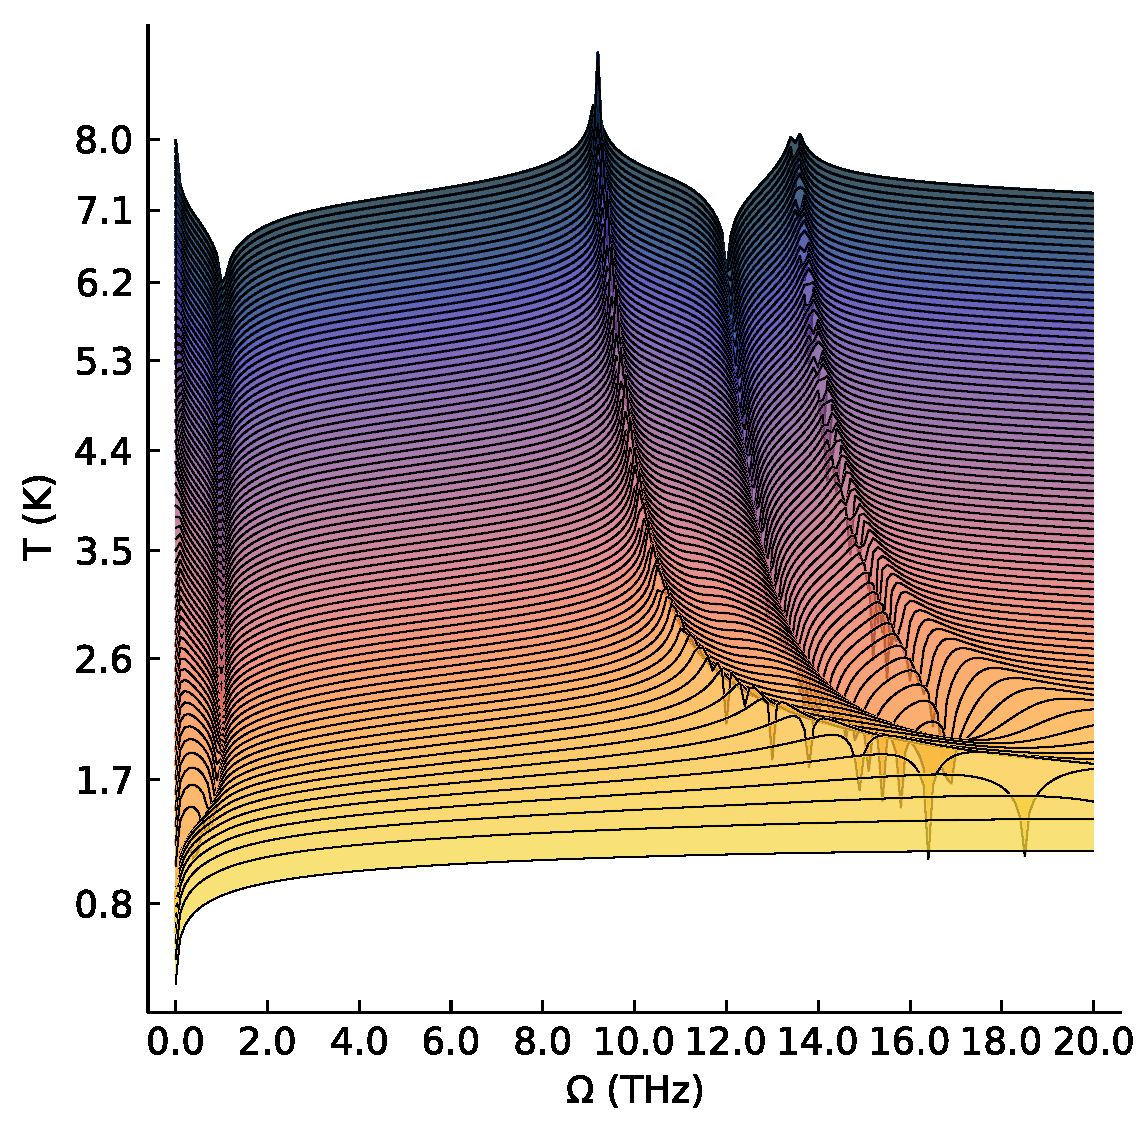
\includegraphics[width=.87\textwidth]{chapters/frohlich/figures/conductivity_plot_temp_imag_9.pdf}
\end{subfigure}%
}
\caption{Ridgeline plots for the real (left) and imaginary (right) complex conductivity at different values of $\alpha$. (a) Real conductivity at $\alpha = 3$. (b) Imaginary conductivity at $\alpha = 3$. (c) Real conductivity at $\alpha = 6$. (d) Imaginary conductivity at $\alpha = 6$. (e) Real conductivity at $\alpha = 9$. (f) Imaginary conductivity at $\alpha = 9$.}
\label{fig:osakaridge}
\end{figure}

\subsection{Polaron mobility in the ``Beyond Quasiparticle'' regime}

\begin{figure}[t]
\vspace*{-1.5cm}\makebox[\linewidth][c]{%
\begin{subfigure}[b]{.6\textwidth}
\centering
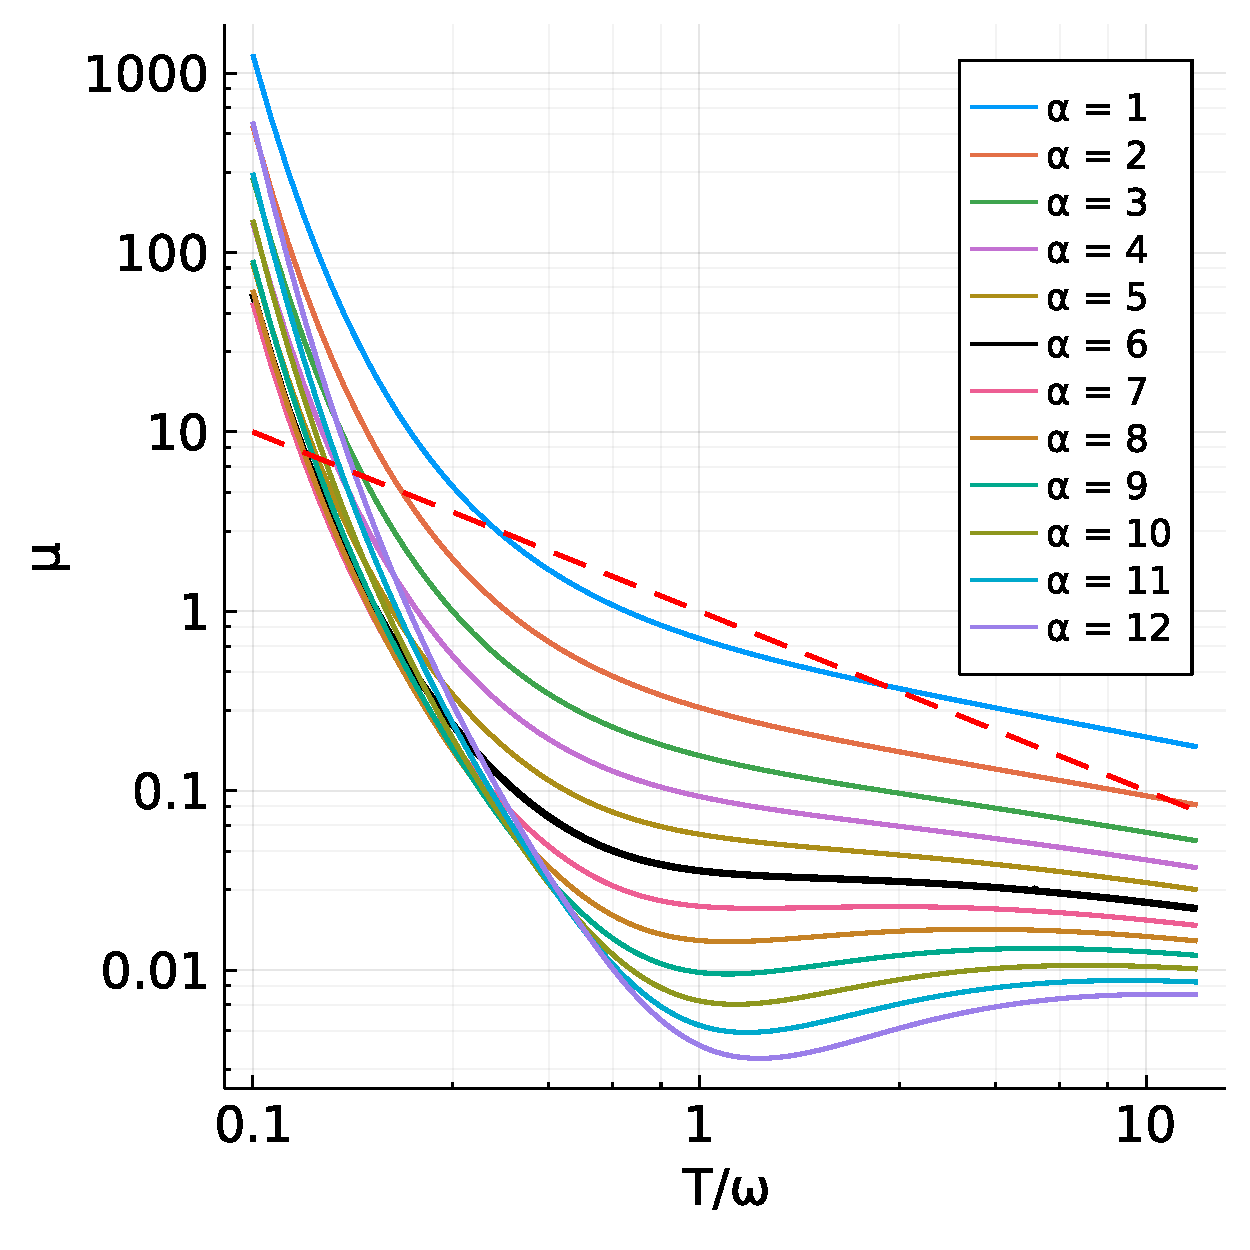
\includegraphics[width=.9\textwidth]{chapters/frohlich/figures/moblility_temp_alpha.pdf}
\end{subfigure}%
\begin{subfigure}[b]{.6\textwidth}
\centering
\includegraphics[width=.9\textwidth]{chapters/frohlich/figures/medium (1).png}
\end{subfigure}%
}
\caption{Temperature dependence of the polaron mobility. The Mott-Ioffe-Regel (MIR) threshold is given by the red dotted lines. Left: Mobility obtained from the thermal FHIP theory with $v$ and $w$ variational parameters calculated for each temperature, for Fr\"ohlich alphas ranging from $\alpha = 1$ to  $12$. The temperature is given in units of the phonon frequency $\omega$. Right: Mobility obtained by~\cite{mishchenko_polaron_2019} using the diagrammatic Monte Carlo method for $\alpha = 6$. The temperature is in units of the phonon frequency $\Omega$.}
\label{fig:mishchenko2}
\end{figure}

\cite{mishchenko_polaron_2019} use the diagrammatic Monte Carlo (DiagMC) method to study the mobility of a Fr\"ohlich polaron in the ``Beyond Quasiparticle'' regime. In this regime, the inelastic scattering rate exceeds the thermal energy of quasiparticles. This can be restated as the regime where the mean free path of the particle exceeds its de Broglie wavelength. In this form, it coincides with the Mott-Ioffe-Regel (MIR) criterion where the motion of quasiparticles is ill-defined. 

In Figure \ref{fig:mishchenko2} are comparisons between the temperature dependence of the polaron mobility evaluated using the~\cite{feynman_mobility_1962} method (right) compared to the~\cite{mishchenko_polaron_2019} DiagMC method (left). The key features of the DiagMC plot (right) are the non-monotonic behaviour of the mobility and the evaluation of the mobility near and below the MIR threshold (given by the red dotted line). These two features are seen in the FHIP mobility too. The main difference between the two results is that, whilst the mobility minimum arises from the DiagMC method at $\alpha = 6$, the minimum arises from the FHIP method at $\alpha \geq 7$ and is less prominent. 

\begin{figure}[t]
\vspace*{-1.5cm}\makebox[\linewidth][c]{%
\begin{subfigure}[b]{.6\textwidth}
\centering
\includegraphics[width=.9\textwidth]{chapters/frohlich/figures/Mischenko_comparison.pdf}
\end{subfigure}%
\begin{subfigure}[b]{.6\textwidth}
\centering
\includegraphics[width=.9\textwidth]{chapters/frohlich/figures/medium.png}
\end{subfigure}%
}
\caption{Polaron mobility for $\alpha = 6$. Left: Mobility obtained from the thermal FHIP theory with $v$ and $w$ variational parameters calculated for each temperature. The electric field frequency and temperature are given in units of the phonon frequency $\omega$. Right: Mobility obtained by~\cite{mishchenko_polaron_2019} using the diagrammatic Monte Carlo method. The electric field frequency and temperature are in units of the phonon frequency $\Omega$.}
\label{fig:mishchenko}
\end{figure}

The mobility evaluated below the MIR threshold is stated in~\cite{mishchenko_polaron_2019} to be ``beyond the quasiparticle'' regime. However, the model from~\cite{feynman_mobility_1962} can reliably evaluate the mobility in this regime too, despite being a quasiparticle model of two fictitious masses coupled by a spring-like potential. Additionally, the FHIP can reproduce the mobility minimum too. \cite{mishchenko_polaron_2019} suggest that the minimum emerges from the competition between the decreasing number of thermal excitations (which dominates for at $T << \omega$) and a strong mass renormalisation (which is prominent for $T \gtrsim \omega$). 

In Figure \ref{fig:mishchenko} are comparisons between the polaron mobility evaluated for a Fr\"ohlich alpha $\alpha = 6$. The left figure shows the polaron mobility obtained from the thermal Feynman polaron theory (evaluated with (Eq. \ref{eqn:FHIP_mobility}) for the dc polaron mobility). The right figure shows the polaron mobility obtained from~\cite{mishchenko_polaron_2019}'s DiagMC method. The position of the peaks between the two methods align for each temperature ($0.125, 0.25, 0.5, 1, 2, 4\  \&\ 8\ K/\omega$, where $\omega$ is the single phonon mode frequency). The main difference between the two methods is that the peaks evaluated from the Feynman polaron method are taller and sharper, whereas the peaks evaluated from~\cite{mishchenko_polaron_2019}'s DiagMC method are broader and shallower. 

The difference in peak widths between the two methods is likely due to the two-mass spring model approximation made in the Feynman method within the trial action in Eq. (\ref{eqn:thermal_trial_action}). This fixes the dynamical behaviour of Feynman's model \emph{a priori} since it only contains two harmonic degrees of freedom. The translation invariance of the Fr\"ohlich Hamiltonian then fixes one eigenmode at zero frequency. The frequency of the other mode and the relative spectral weight of the peaks are then the free parameters. This spectrum differs greatly from the true spectrum of the polaron, and means that the FHIP polaron mobility may only contain a very crude approximation of the true dissipation of the polaron. The dynamical properties of the FHIP approximation is investigated more by~\cite{sels_dynamic_2016}.

\begin{figure}
\vspace*{-1.5cm}\makebox[\linewidth][c]{%
\begin{subfigure}[t]{0.01\textwidth}
    \vspace*{-7.5cm}\textbf{a}
  \end{subfigure}%
\begin{subfigure}[b]{.58\textwidth}
\centering
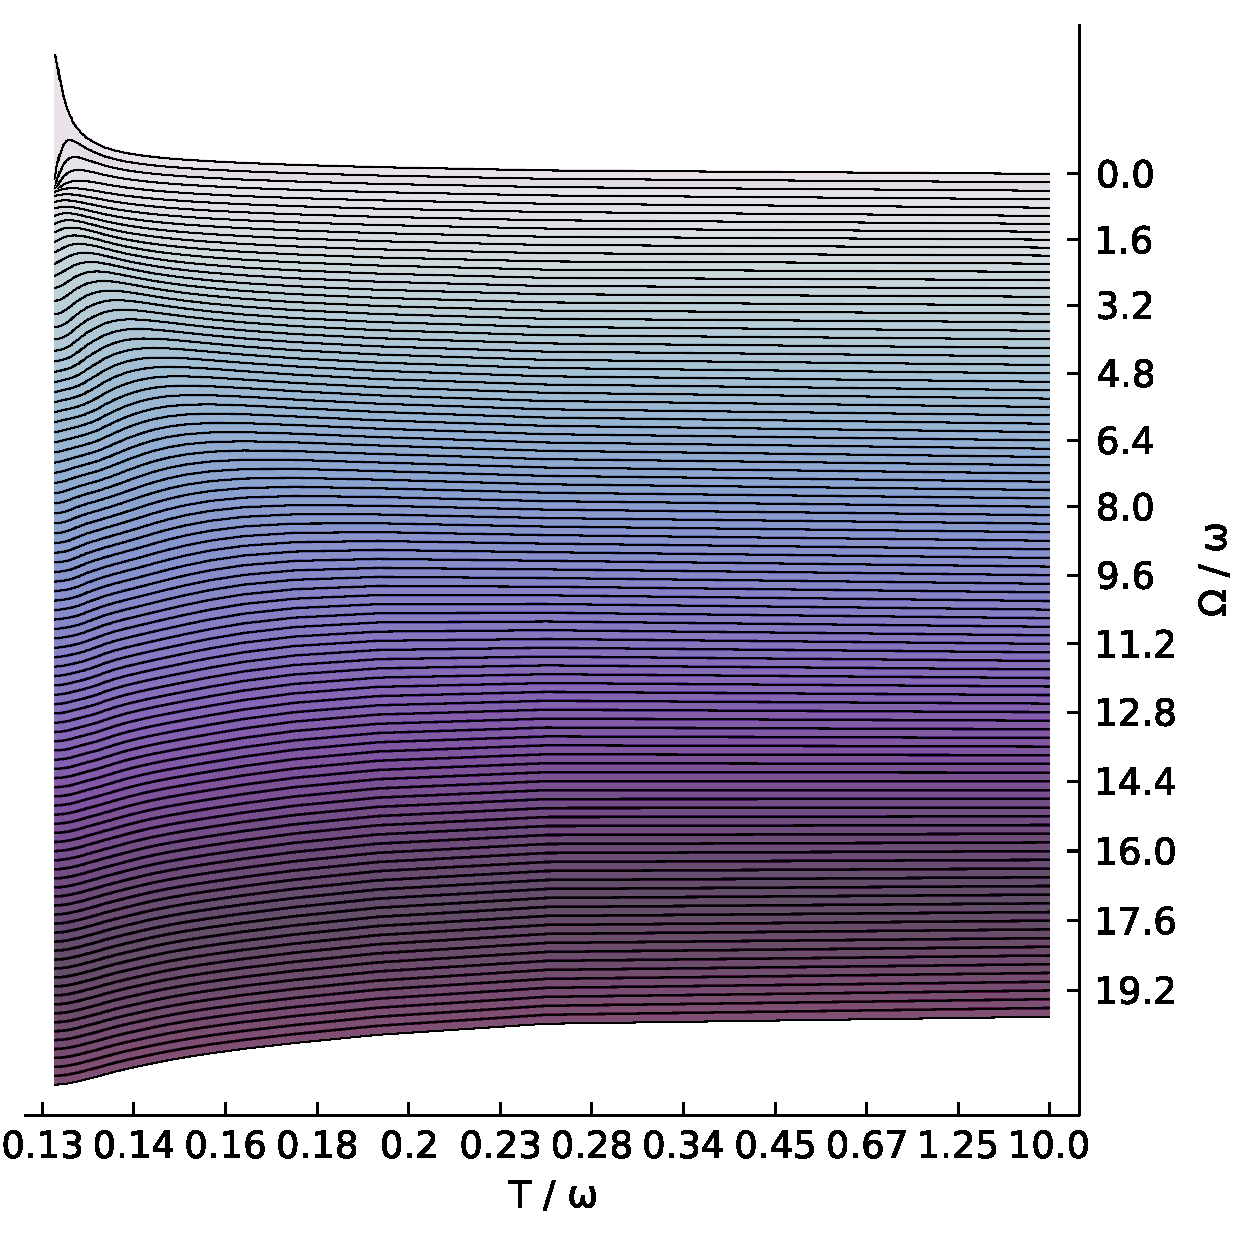
\includegraphics[width=.9\textwidth]{chapters/frohlich/figures/conductivity_plot_freq_real_3.pdf}
\end{subfigure}%
\begin{subfigure}[t]{0.01\textwidth}
    \vspace*{-7.5cm}\textbf{b}
  \end{subfigure}
\begin{subfigure}[b]{.58\textwidth}
\centering
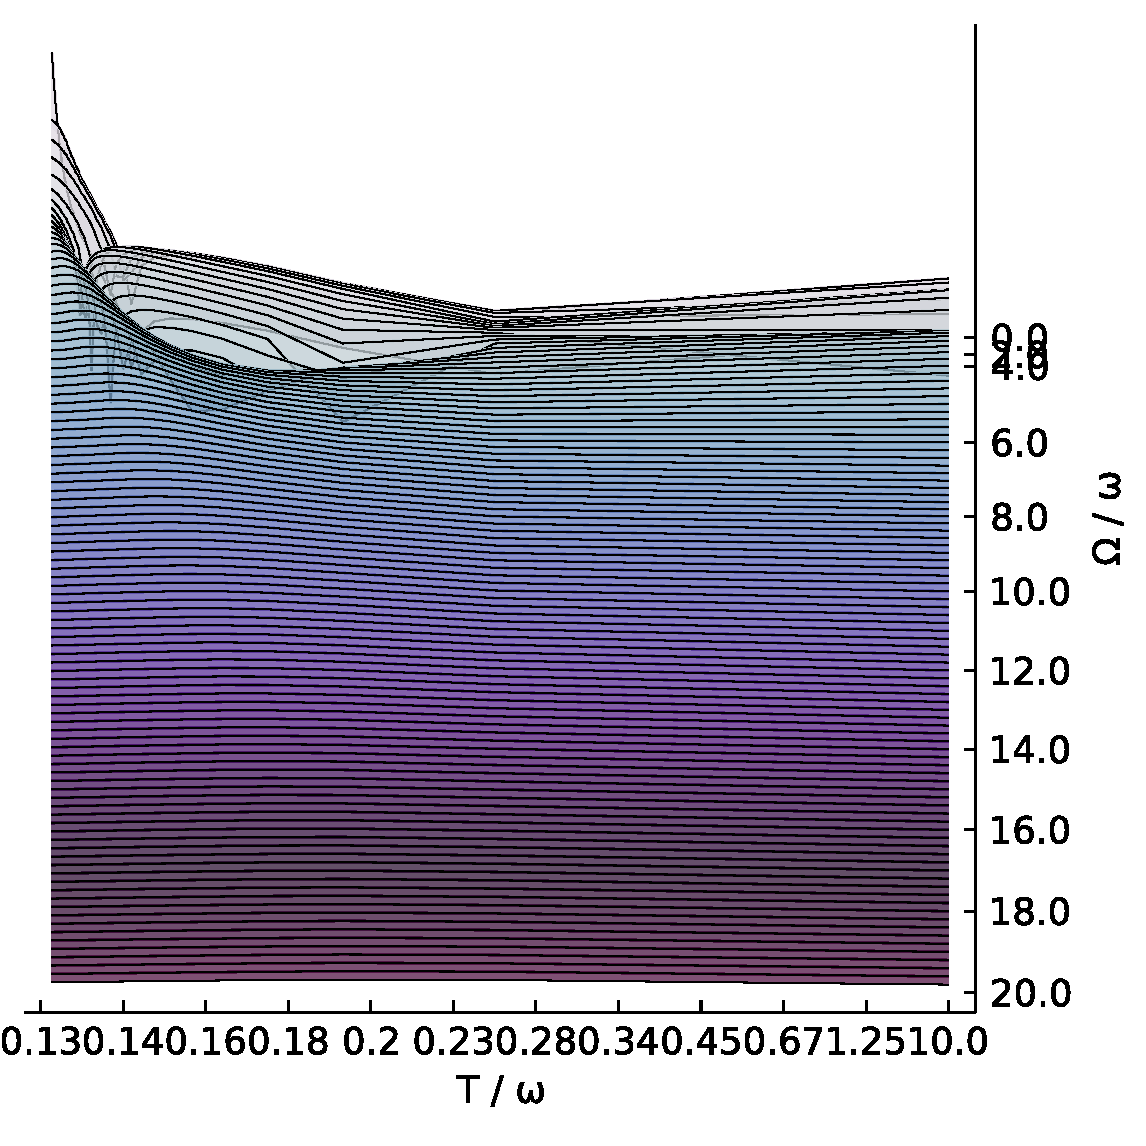
\includegraphics[width=.9\textwidth]{chapters/frohlich/figures/conductivity_plot_freq_imag_3.pdf}
\end{subfigure}%
}\\
\makebox[\linewidth][c]{%
\begin{subfigure}[t]{0.01\textwidth}
    \vspace*{-7.5cm}\textbf{c}
  \end{subfigure}%
\begin{subfigure}[b]{.58\textwidth}
\centering
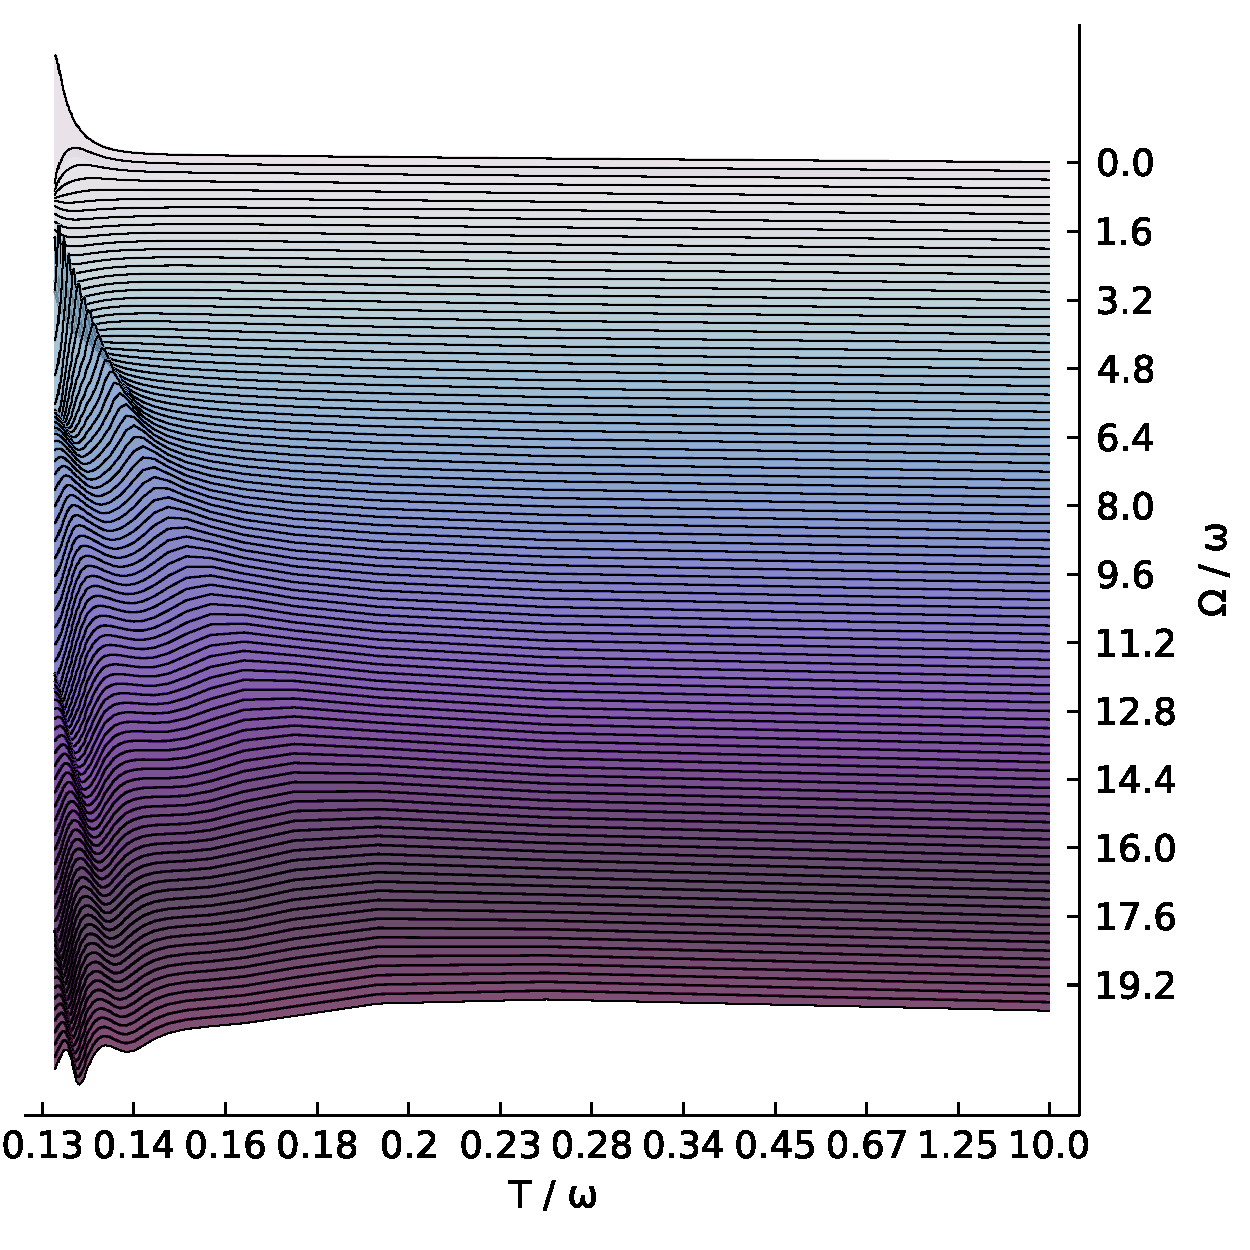
\includegraphics[width=.9\textwidth]{chapters/frohlich/figures/conductivity_plot_freq_real_6.pdf}
\end{subfigure}%
\begin{subfigure}[t]{0.01\textwidth}
    \vspace*{-7.5cm}\textbf{d}
  \end{subfigure}%
\begin{subfigure}[b]{.58\textwidth}
\centering
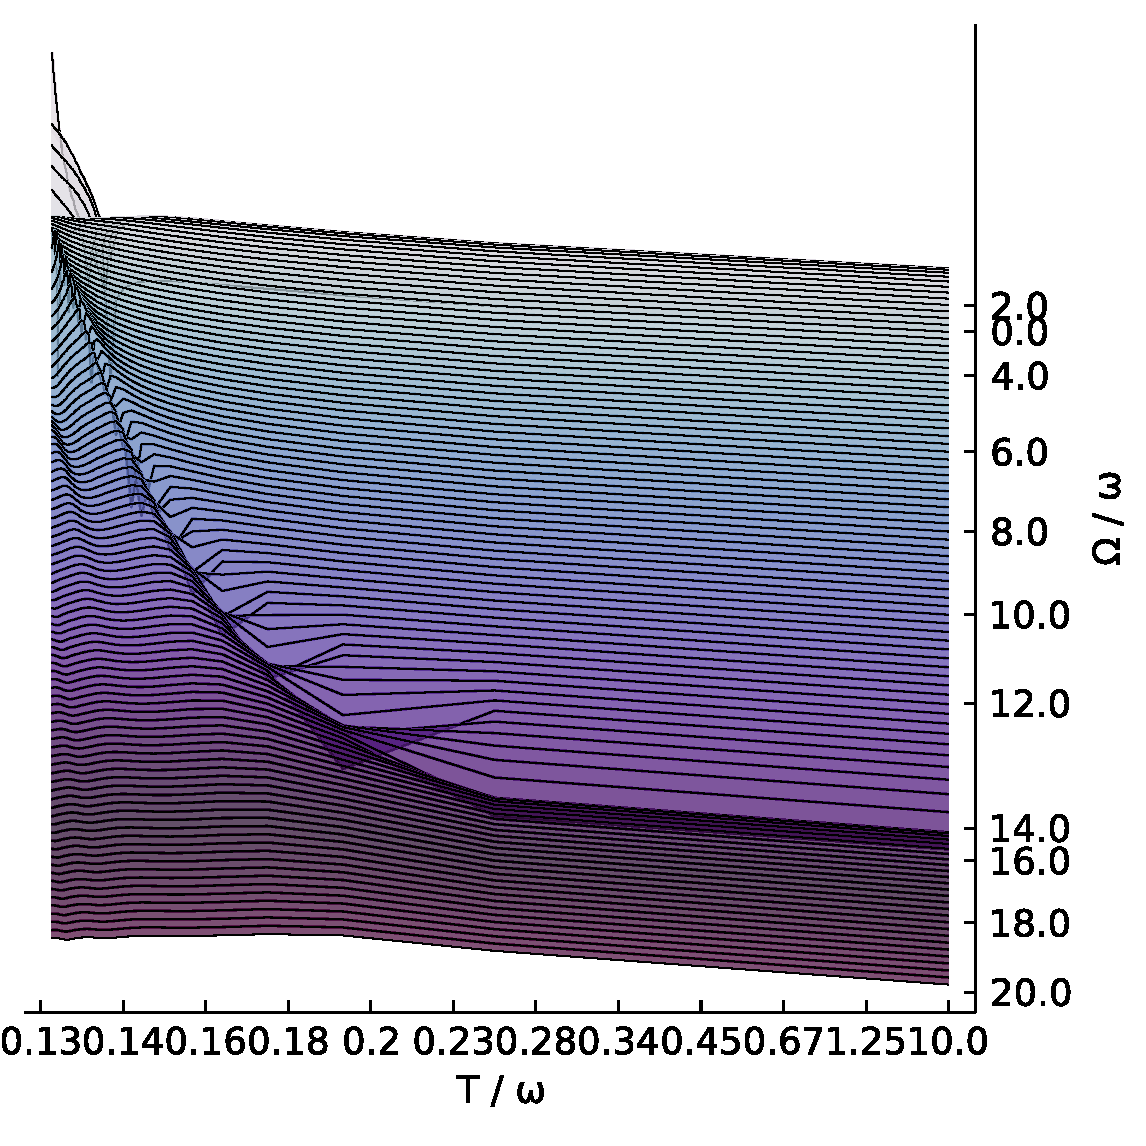
\includegraphics[width=.9\textwidth]{chapters/frohlich/figures/conductivity_plot_freq_imag_6.pdf}
\end{subfigure}%
}
\makebox[\linewidth][c]{%
\begin{subfigure}[t]{0.01\textwidth}
    \vspace*{-7.5cm}\textbf{e}
  \end{subfigure}%
\begin{subfigure}[b]{.58\textwidth}
\centering
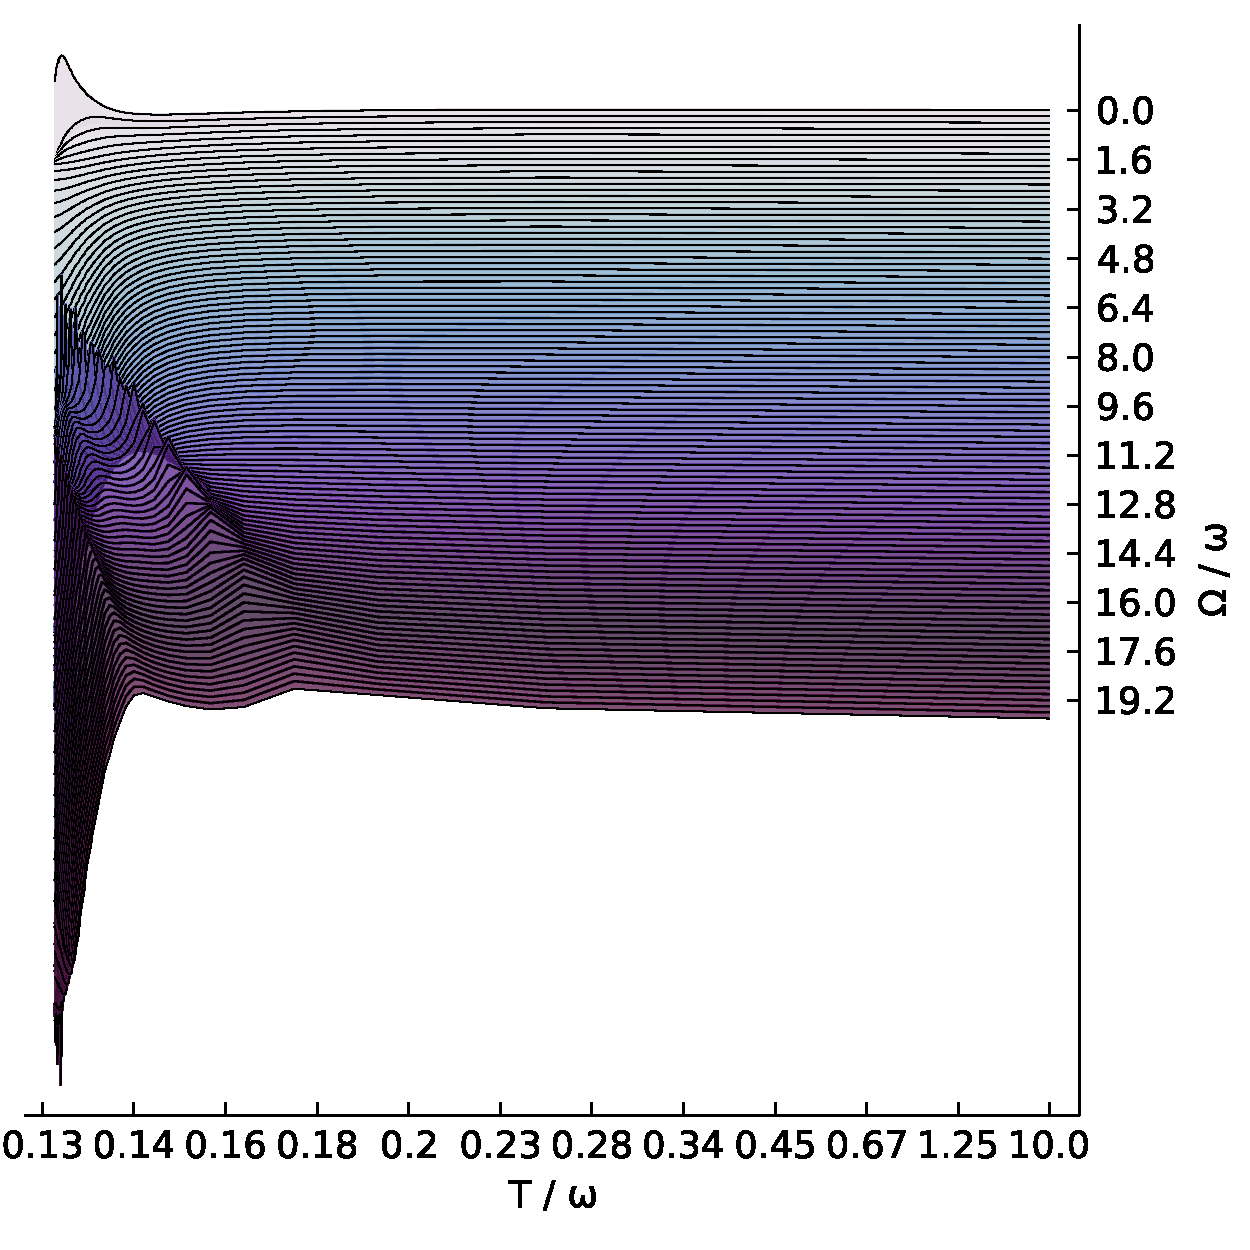
\includegraphics[width=.9\textwidth]{chapters/frohlich/figures/conductivity_plot_freq_real_9.pdf}
\end{subfigure}%
\begin{subfigure}[t]{0.01\textwidth}
    \vspace*{-7.5cm}\textbf{f}
  \end{subfigure}%
\begin{subfigure}[b]{.58\textwidth}
\centering
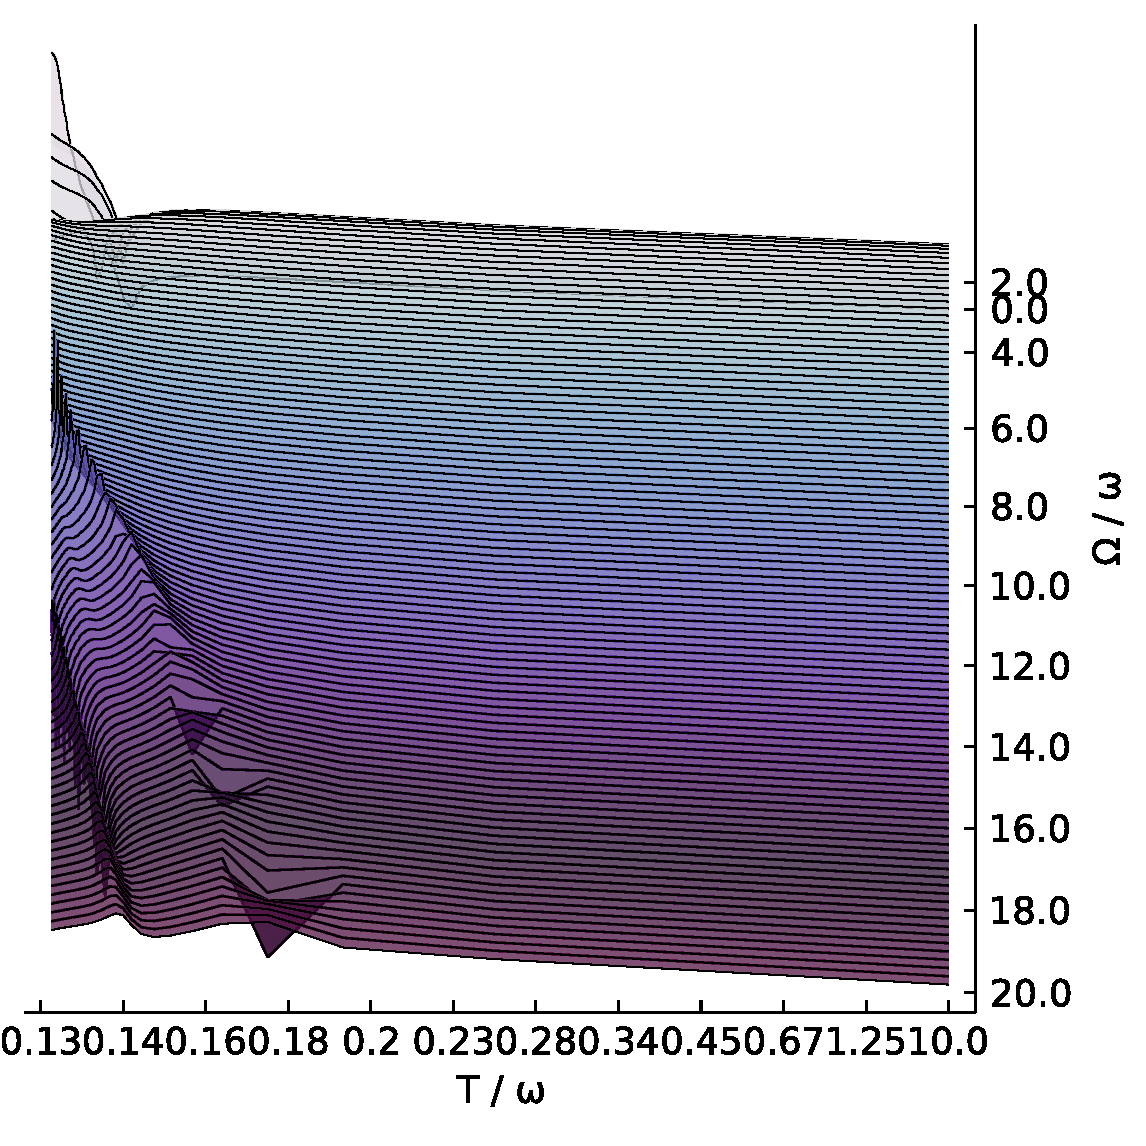
\includegraphics[width=.9\textwidth]{chapters/frohlich/figures/conductivity_plot_freq_imag_9.pdf}
\end{subfigure}%
}
\caption{The same ridgeline plots as in Figure 5 but with the y- and x-axes swapped. }
\end{figure}

\ection{Multiple Phonon Modes}

\begin{table}
\begin{center}
\begin{tabular}{||c|c|c|c||} 
\hline\hline
Phonon Frequencies (THz) & IR Activity & $\epsilon^{\text{ionic}}_j$ & $\alpha_j$ \\
\hline\hline
4.017 & 0.082 & 0.300 & 0.034 \\
\hline
3.888 & 0.006 & 0.025 & 0.003 \\
\hline
3.531 & 0.054 & 0.254 & 0.031 \\ 
\hline
2.755 & 0.021 & 0.166 & 0.023 \\
\hline
2.438 & 0.232 & 2.308 & 0.336 \\
\hline
2.249 & 0.262 & 3.071 & 0.465 \\
\hline
2.080 & 0.234 & 3.203 & 0.505 \\
\hline
2.034 & 0.062 & 0.893 & 0.142 \\
\hline
1.567 & 0.037 & 0.886 & 0.161 \\
\hline
1.019 & 0.013 & 0.721 & 0.162 \\
\hline
1.002 & 0.007 & 0.402 & 0.091 \\
\hline
0.997 & 0.010 & 0.618 & 0.141 \\
\hline
0.920 & 0.011 & 0.767 & 0.182 \\
\hline
0.801 & 0.002 & 0.156 & 0.040 \\
\hline
0.574 & 0.007 & 1.163 & 0.349 \\
\hline\hline
\end{tabular} \label{table:mapidata}
\caption{Infrared activity, ionic dielectric contribution and decomposed Fr\"ohlich alpha values associated with each of the phonon modes in MAPbI3 taken from Ref~\cite{brivio_lattice_2015}. The effective Fr\"ohlich alpha $\alpha_{\text{eff}} = \sum_j \alpha_j$ is found to be $2.66$ for MAPbI3.}
\end{center}
\end{table}

I have produced a Julia Pluto.jl notebook that uses the multiple phonon theory to evaluate the decomposed Fr\"ohlich $\alpha_j$ components associated with $15$ modes of Methylammonium lead iodide (MAPbI$_3$). The frequencies and infrared activities associated with these modes are listed in Table 1. The decomposed $\alpha_j$ parameters and phonon frequencies $\omega_j$ are then inserted into the variational principle for multiple phonons to obtain a $v$ and $w$ parameter that provide the lowest upper-bound to the exact free energy of the multi-modal polaron system. The two effective phonon frequencies schemes, labelled scheme A and B in~\cite{hellwarth_mobility_1999} (c.f. section 3.6.5), evaluate the Fr\"ohlich alpha for MAPbI$_3$ to be $\alpha = 2.52$ (towards zero temperature the A scheme gives a slightly different value of $2.44$). In comparison, including the ionic contributions of each MAPbI$_3$ phonon modes explicitly produced the decomposed Fr\"ohlich alpha $\alpha_j$ shown in Table 1. From these, I obtain an effective alpha for MAPbI$_3$ of $\alpha_{\text{eff}} = 2.66$ which is only slightly larger than the value predicted by the effective mode A and B schemes. The free energy approximated by the multiple phonon theory is shown in comparison the Hellwarth and Biaggio effective mode theory in Figure \ref{fig:multitheory}a. The two Hellwarth schemes agree for almost all temperatures except for a small deviation towards zero temperature where the A scheme gives a slightly lower value. The multiple phonon theory clearly gives a lower estimate to the free energy of the polaron compared to the Hellwarth theory for all temperatures above roughly $100$K but gives a higher value at lower temperatures and at zero temperature. Figure \ref{fig:multitheory}b shows a comparison between the multiple phonon variational $v$ and $w$ parameters compared to the effective variational parameters from the Hellwarth and Biaggio effective mode theory. The two agree at zero temperature, but the multiple phonon theory predicts larger polaron frequencies at higher temperatures and a smaller different in $v$ and $w$, $v - w$, at all temperatures. 

\begin{figure}[t]
\vspace*{-1.5cm}\makebox[\linewidth][c]{%
\begin{subfigure}[b]{.6\textwidth}
\centering
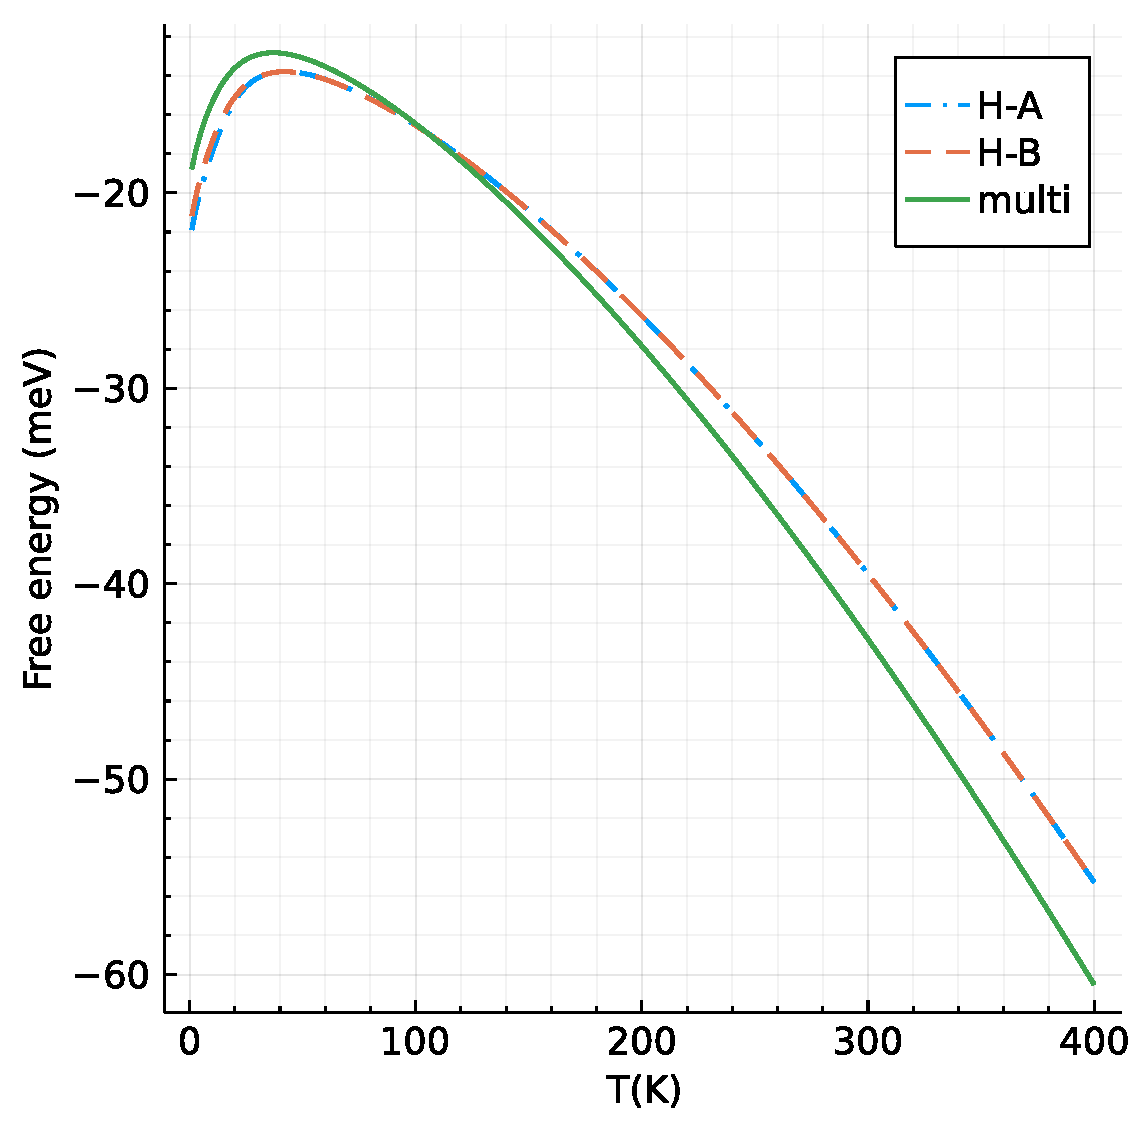
\includegraphics[width=.9\textwidth]{chapters/frohlich/figures/free_energy_temp.pdf}
\end{subfigure}%
\begin{subfigure}[b]{.6\textwidth}
\centering
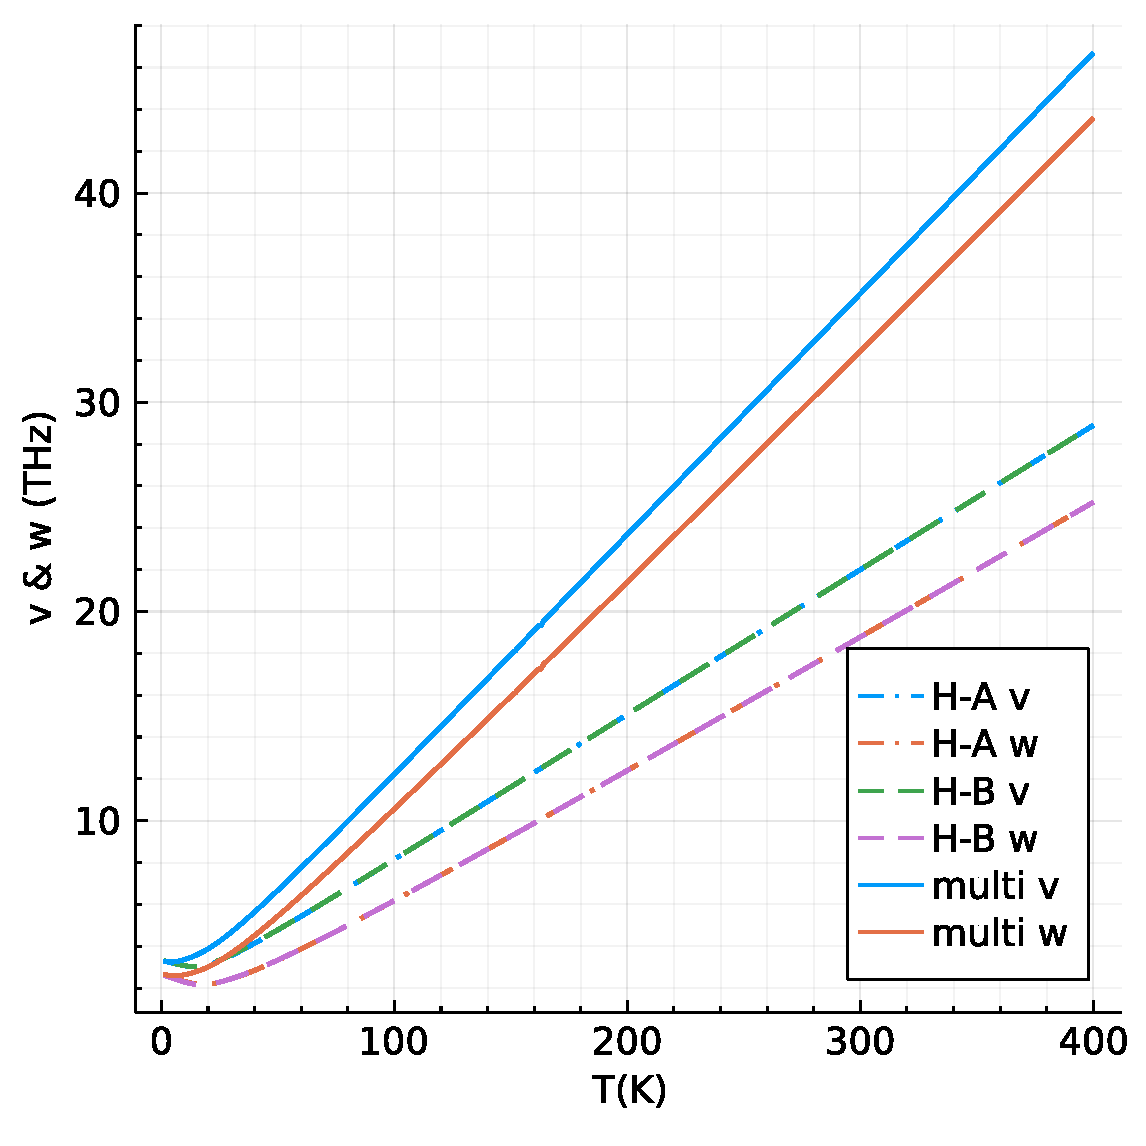
\includegraphics[width=.9\textwidth]{chapters/frohlich/figures/vw_temp.pdf}
\end{subfigure}%
}
\caption{(left): The free energy of the Hellwarth and Biaggio effective mode A \& B schemes and for the multiple phonon model between $1$K and $400$K. The two Hellwarth schemes agree almost exactly except for a small deviation at low temperatures. The multiple phonon model gives a lower free energy estimate for temperatures above $100$K. (right): The variational parameters $v$ \& $w$ from the Hellwarth and Biaggio effective mode A \& B schemes and the multiple phonon model. The effective mode schemes agree whereas the multiple phonon model gives values larger than the Hellwarth schemes but approaches their values towards zero temperature.}
\label{fig:multitheory}
\end{figure}

Figures \ref{fig:multicontour} (contour plots) and \ref{fig:multiridge} (ridge-line plots) compare the complex conductivity obtained from the multiple phonon model (left column) to the complex conductivity obtained from the Hellwarth and Biaggio B scheme (right column). The top rows show the real part of the conductivity (i.e. the ac mobility), the middle rows show the imaginary part and the bottom rows show the absolute value. I chose the B scheme over the A scheme because the B scheme involves matching an effective frequency to the full extent of \=Osaka's finite temperature variational principle, so is arguably more accurate. On the other hand, the A scheme produces a temperature-dependent Fr\"ohlich alpha parameter and effective phonon frequency. This is unlike the original Fr\"ohlich alpha and phonon frequency which are independent of temperature. Nonetheless, the two schemes do produce near-identical results for most temperature anyway, except for a slight deviation at very low temperatures. So, a lot of the comparison with the B scheme will be comparable to that of the A scheme too. 

Both the multiple phonon theory and the Hellwarth and Biaggio effective mode theory have similar dc mobilities and high temperature complex conductivities. Likewise, they both possess a broad peak starting around a frequency of $2.03$ THz, which is the effective phonon frequency derived from the B scheme. (At zero temperature, the A scheme gives an effective phonon frequency of $2.17$ THz). The start of the main peak then shifts up in frequency as the temperature increases whilst primarily broadening and flattening. The theories differ in their frequency dependence. Whilst both possess the same main peak starting around $2$ THz, the multiple phonon theory possesses extra peaks below $2$ THz, particular two fairly sharp peaks starting around $0.50$ THz and $1.00$ THz. All of these extra details are washed-out at higher temperatures to leave one main broad peak that has a maximum located at a slightly lower frequency compared to Hellwarth's and Biaggio's theory.

\begin{figure}
\vspace*{-1.5cm}\makebox[\linewidth][c]{%
\begin{subfigure}[t]{0.01\textwidth}
    \vspace*{-8.1cm}\hspace*{9.3cm}\textbf{\underline{Real}}
    \vspace*{-7.5cm}\textbf{a}
  \end{subfigure}%
\begin{subfigure}[b]{.6\textwidth}
\centering
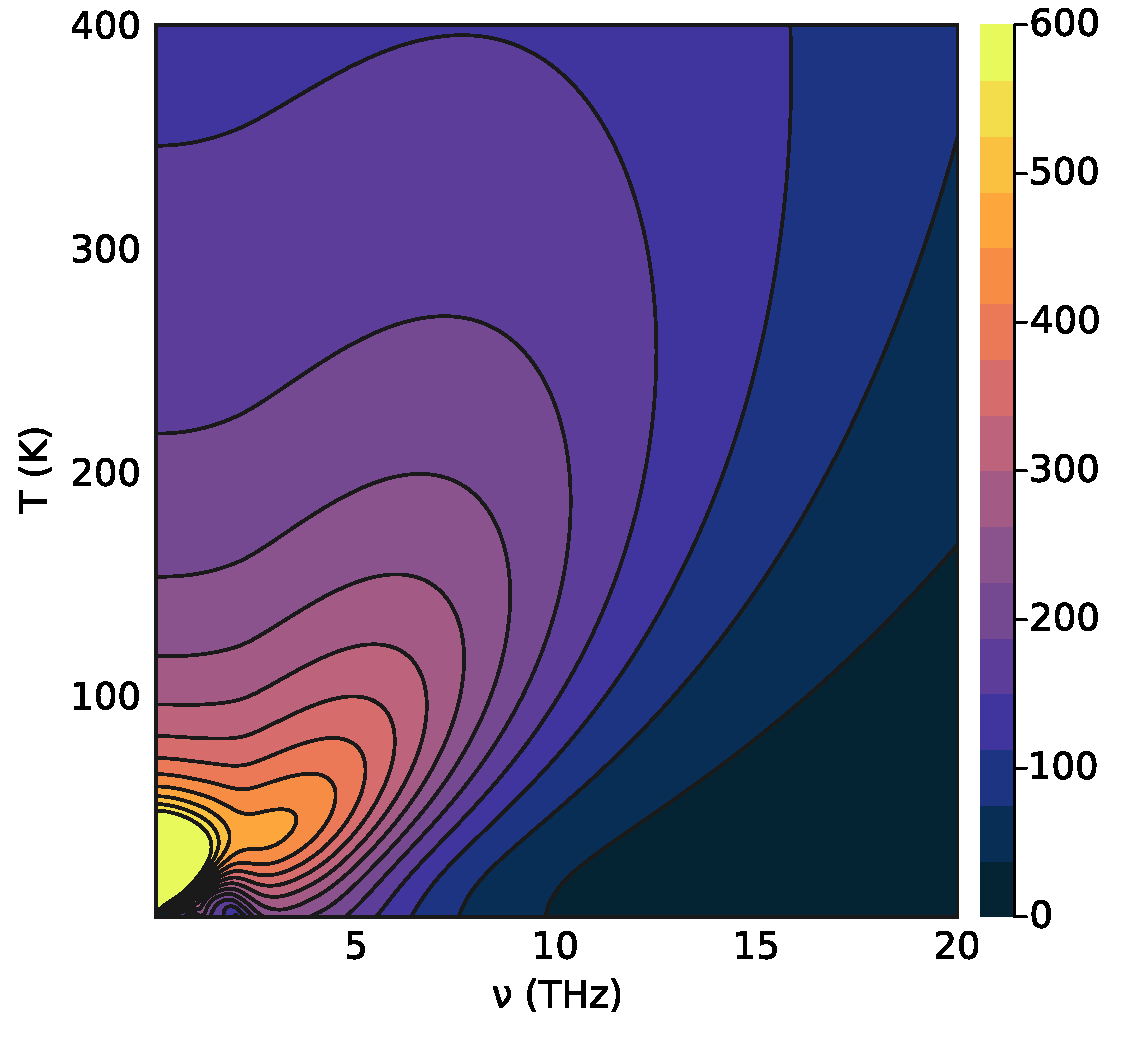
\includegraphics[width=.9\textwidth]{chapters/frohlich/figures/multi_contour_real.pdf}
\end{subfigure}%
\begin{subfigure}[t]{0.01\textwidth}
    \vspace*{-7.5cm}\textbf{b}
  \end{subfigure}
\begin{subfigure}[b]{.6\textwidth}
\centering
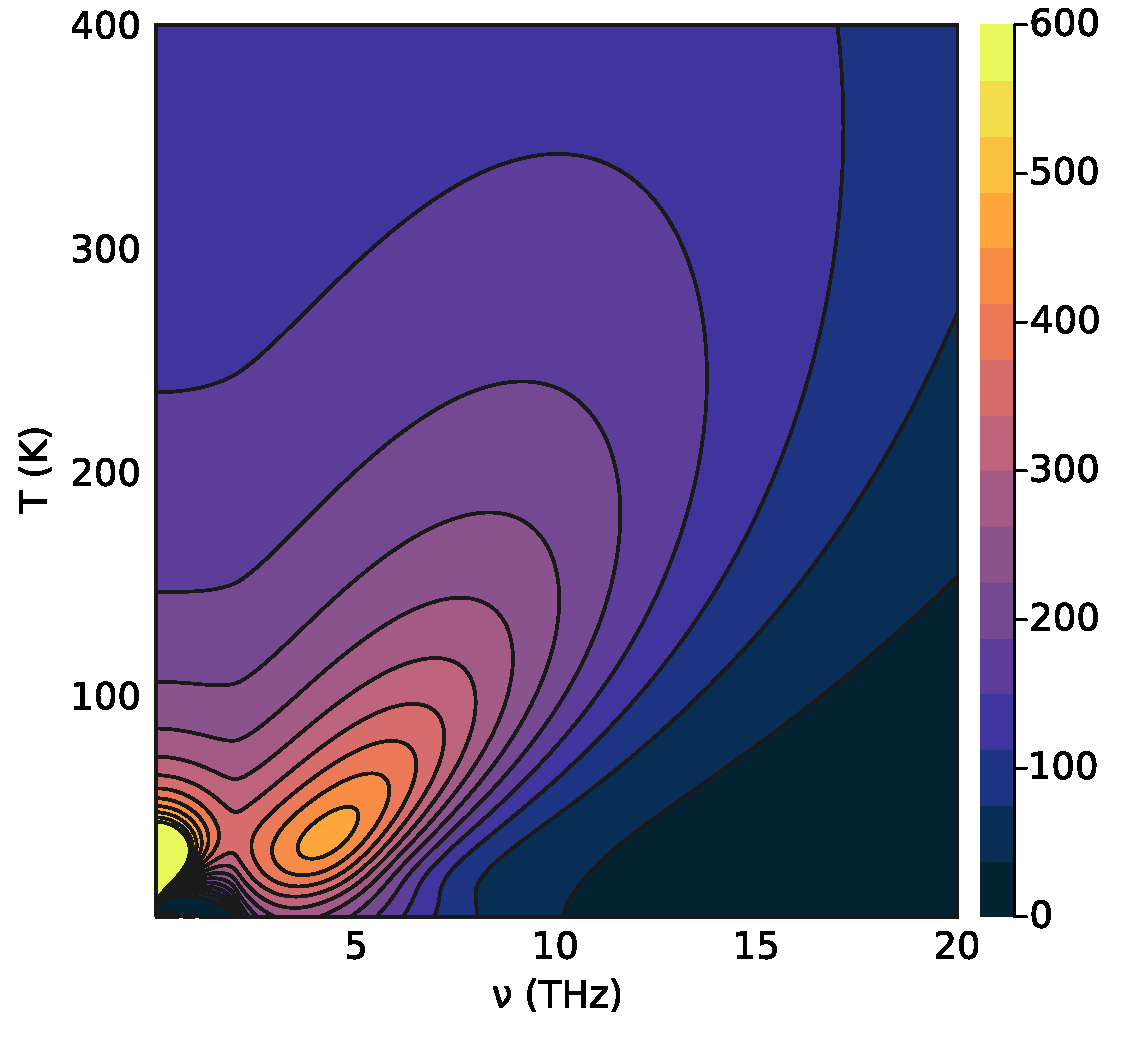
\includegraphics[width=.9\textwidth]{chapters/frohlich/figures/B_contour_real.pdf}
\end{subfigure}%
}\\
\makebox[\linewidth][c]{%
\begin{subfigure}[t]{0.01\textwidth}
    \vspace*{-8.1cm}\hspace*{9.3cm}\textbf{\underline{Imag}}
    \vspace*{-7.5cm}\textbf{c}
  \end{subfigure}%
\begin{subfigure}[b]{.6\textwidth}
\centering
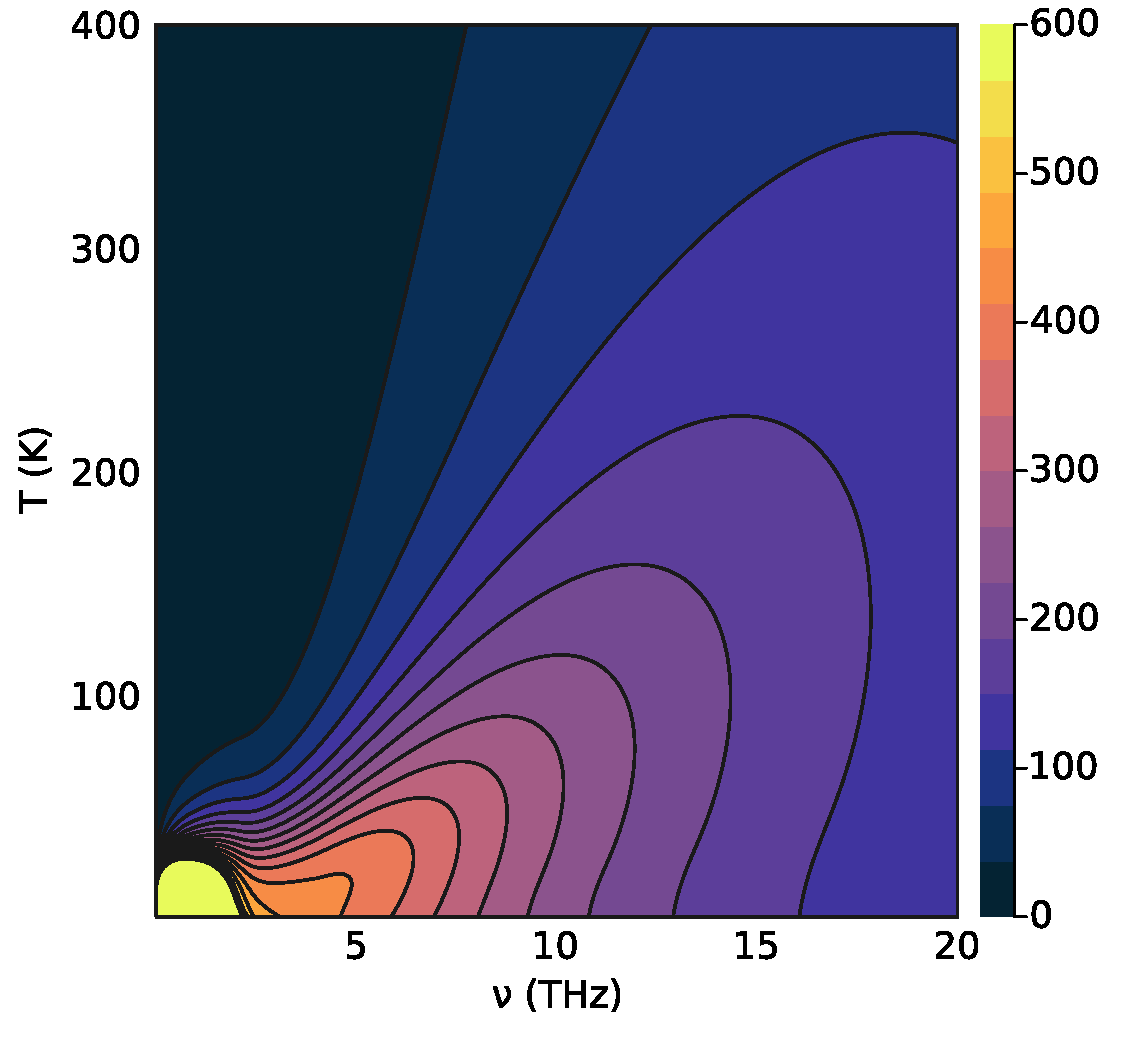
\includegraphics[width=.9\textwidth]{chapters/frohlich/figures/multi_contour_imag.pdf}
\end{subfigure}%
\begin{subfigure}[t]{0.01\textwidth}
    \vspace*{-7.5cm}\textbf{d}
  \end{subfigure}%
\begin{subfigure}[b]{.6\textwidth}
\centering
\includegraphics[width=.9\textwidth]{chapters/frohlich/figures/B_contour_imag.pdf}
\end{subfigure}%
}
\makebox[\linewidth][c]{%
\begin{subfigure}[t]{0.01\textwidth}
    \vspace*{-8.1cm}\hspace*{9.3cm}\textbf{\underline{Abs}}
    \vspace*{-7.5cm}\textbf{e}
  \end{subfigure}%
\begin{subfigure}[b]{.6\textwidth}
\centering
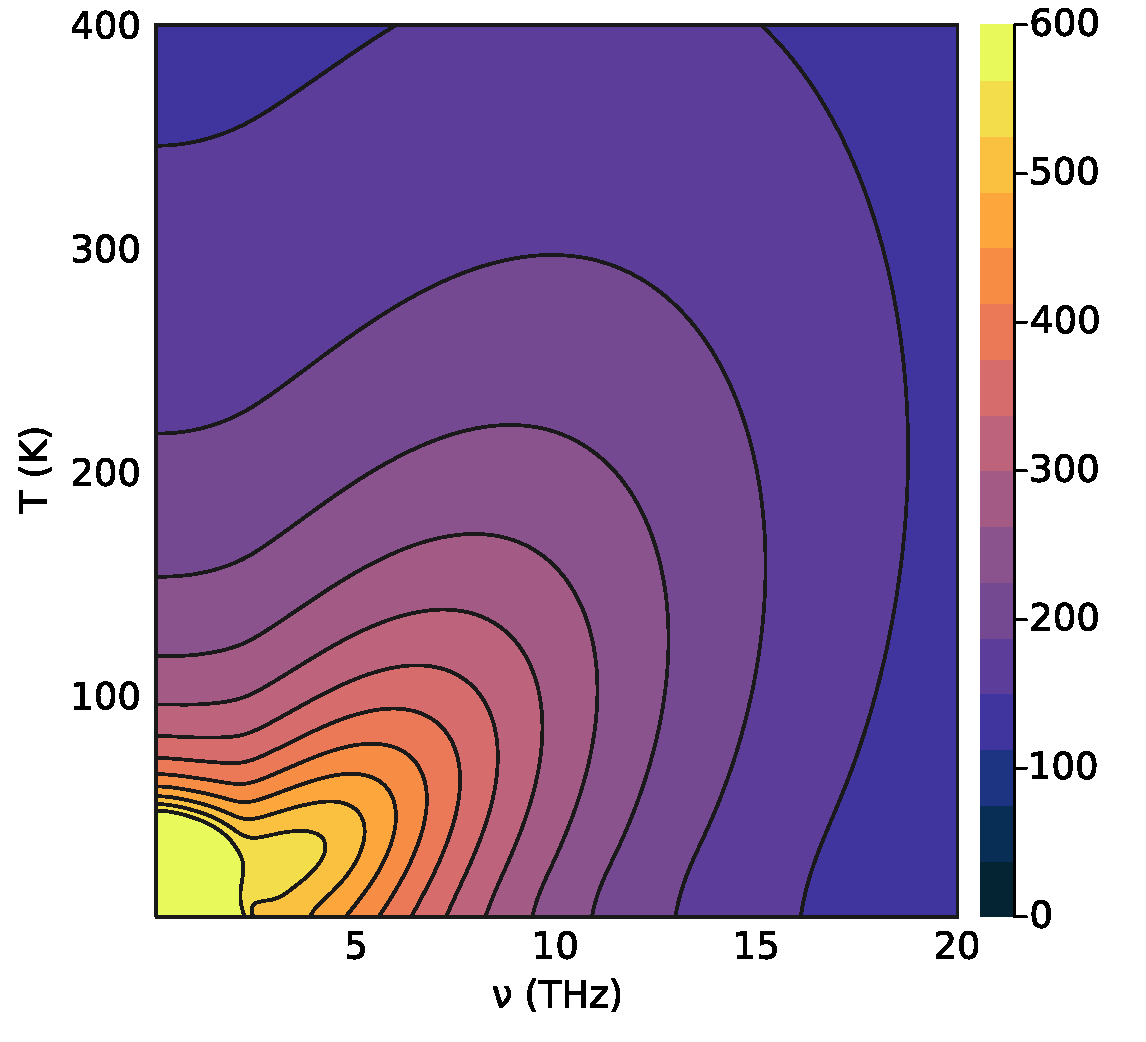
\includegraphics[width=.9\textwidth]{chapters/frohlich/figures/multi_contour_abs.pdf}
\end{subfigure}%
\begin{subfigure}[t]{0.01\textwidth}
    \vspace*{-7.5cm}\textbf{f}
  \end{subfigure}%
\begin{subfigure}[b]{.6\textwidth}
\centering
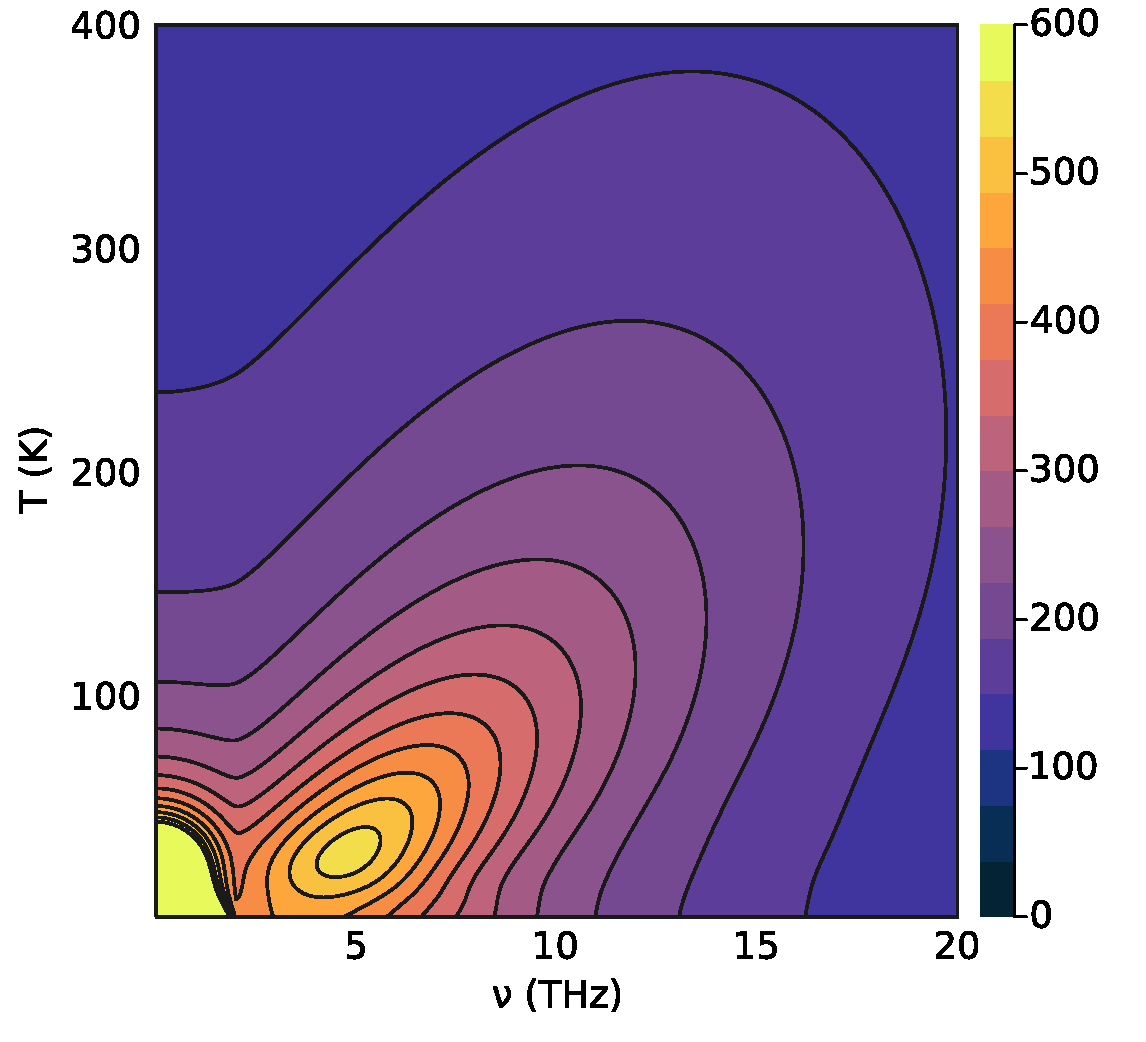
\includegraphics[width=.9\textwidth]{chapters/frohlich/figures/B_contour_abs.pdf}
\end{subfigure}%
}
\caption{Left: Multiple phonon scheme (a) real conductivity, (c) imaginary conductivity, (e) absolute conductivity. Right: Hellwarth `B' scheme: (b) real conductivity, (d) imaginary conductivity, (f) absolute conductivity.}
\label{fig:multicontour}
\end{figure}

\begin{figure}
\vspace*{-1.5cm}\makebox[\linewidth][c]{%
\begin{subfigure}[t]{0.01\textwidth}
    \vspace*{-8.1cm}\hspace*{9cm}\textbf{\underline{Real}}
    \vspace*{-7.5cm}\textbf{a}
  \end{subfigure}%
\begin{subfigure}[b]{.58\textwidth}
\centering
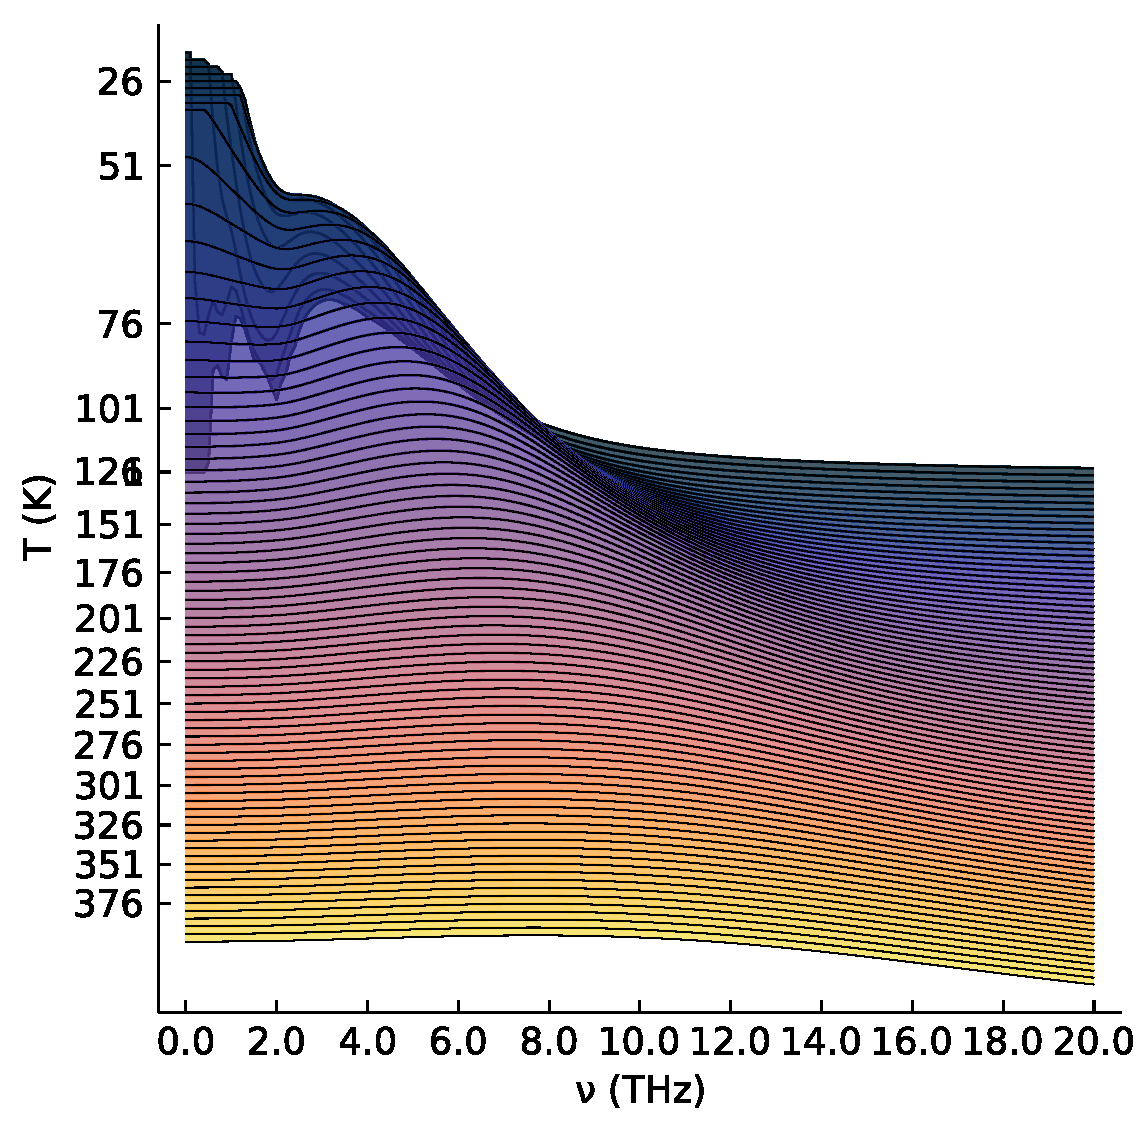
\includegraphics[width=.88\textwidth]{chapters/frohlich/figures/multi_plot_temp_real.pdf}
\end{subfigure}%
\begin{subfigure}[t]{0.01\textwidth}
    \vspace*{-7.5cm}\textbf{b}
  \end{subfigure}
\begin{subfigure}[b]{.58\textwidth}
\centering
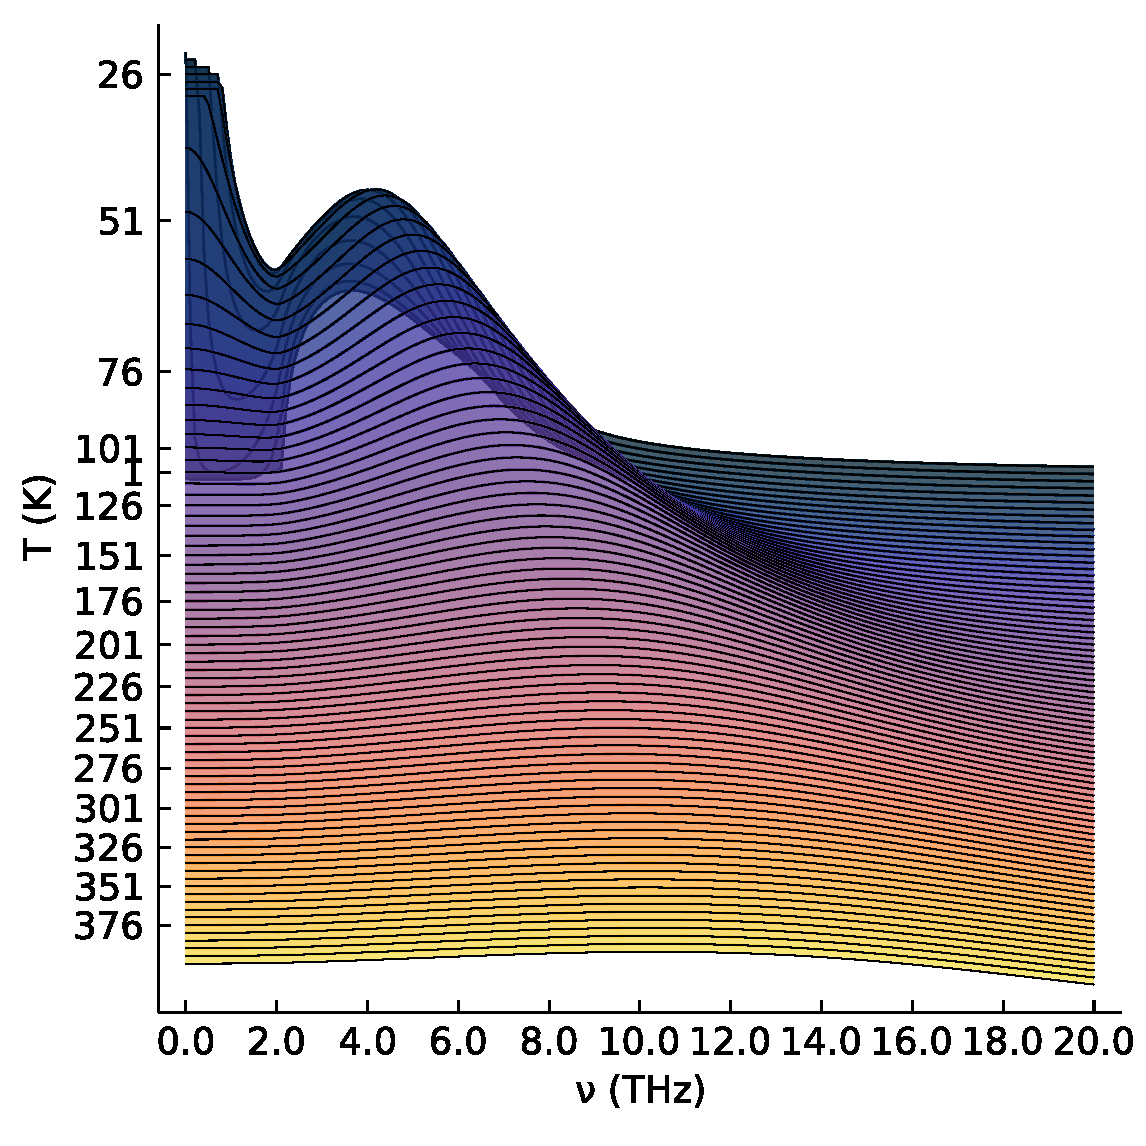
\includegraphics[width=.88\textwidth]{chapters/frohlich/figures/B_plot_temp_real.pdf}
\end{subfigure}%
}\\
\makebox[\linewidth][c]{%
\begin{subfigure}[t]{0.01\textwidth}
    \vspace*{-8.1cm}\hspace*{9cm}\textbf{\underline{Imag}}
    \vspace*{-7.5cm}\textbf{c}
  \end{subfigure}%
\begin{subfigure}[b]{.58\textwidth}
\centering
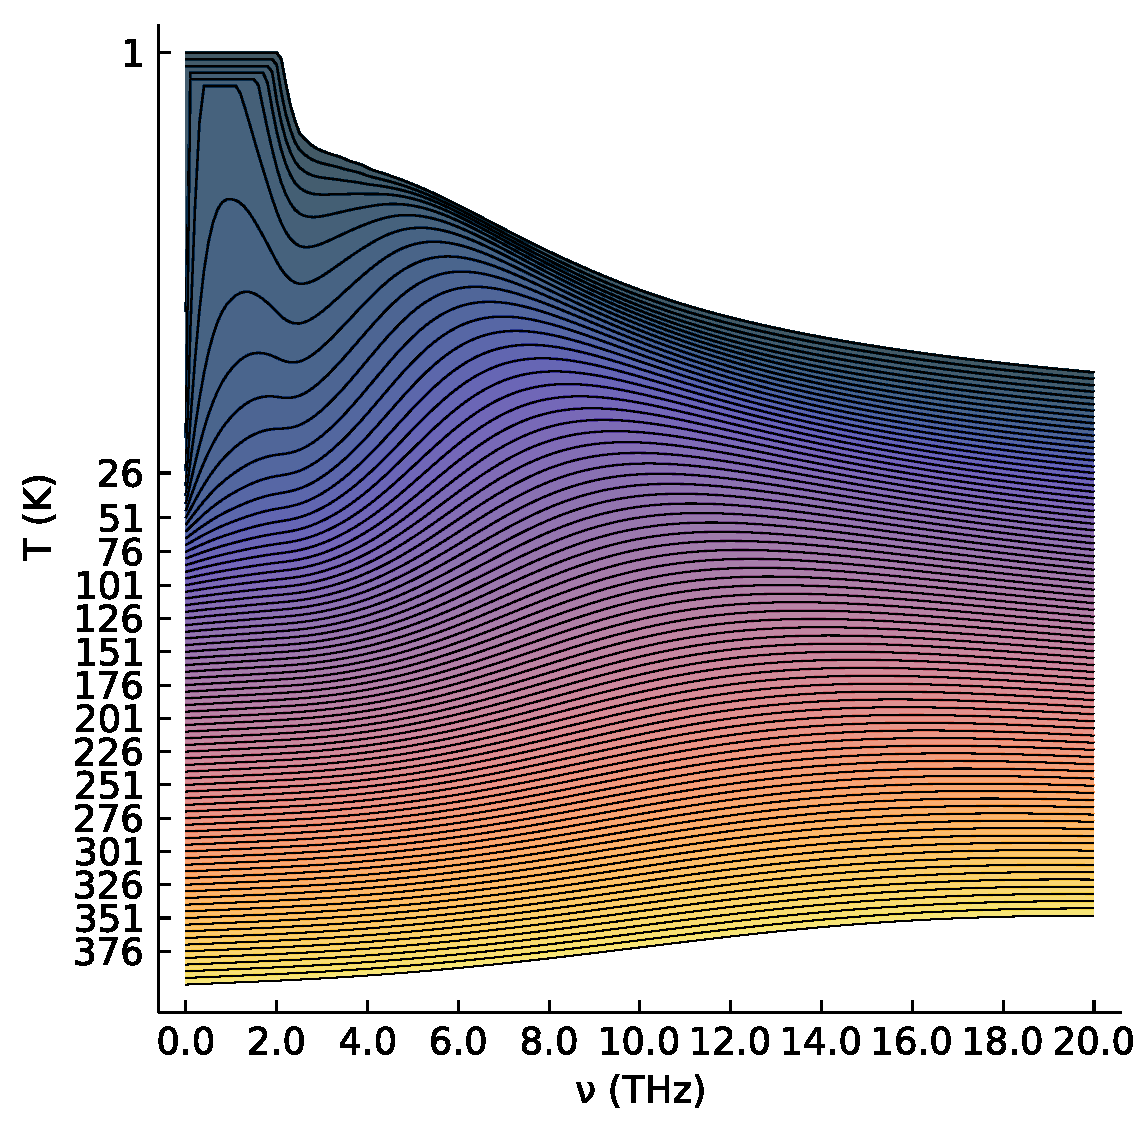
\includegraphics[width=.88\textwidth]{chapters/frohlich/figures/multi_plot_temp_imag.pdf}
\end{subfigure}%
\begin{subfigure}[t]{0.01\textwidth}
    \vspace*{-7.5cm}\textbf{d}
  \end{subfigure}%
\begin{subfigure}[b]{.58\textwidth}
\centering
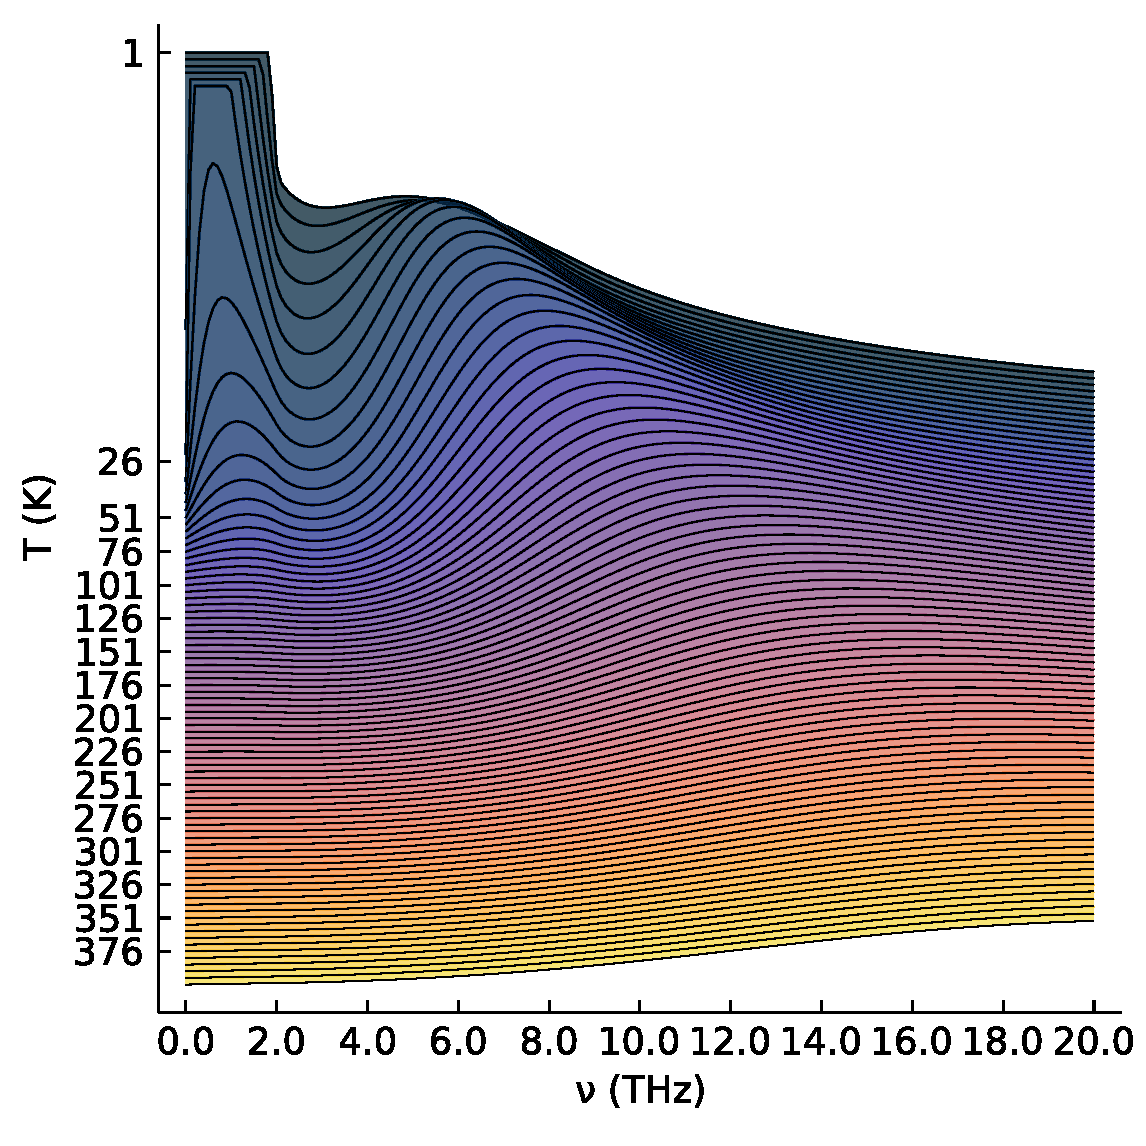
\includegraphics[width=.88\textwidth]{chapters/frohlich/figures/B_plot_temp_imag.pdf}
\end{subfigure}%
}
\makebox[\linewidth][c]{%
\begin{subfigure}[t]{0.01\textwidth}
    \vspace*{-8.1cm}\hspace*{9cm}\textbf{\underline{Abs}}
    \vspace*{-7.5cm}\textbf{e}
  \end{subfigure}%
\begin{subfigure}[b]{.58\textwidth}
\centering
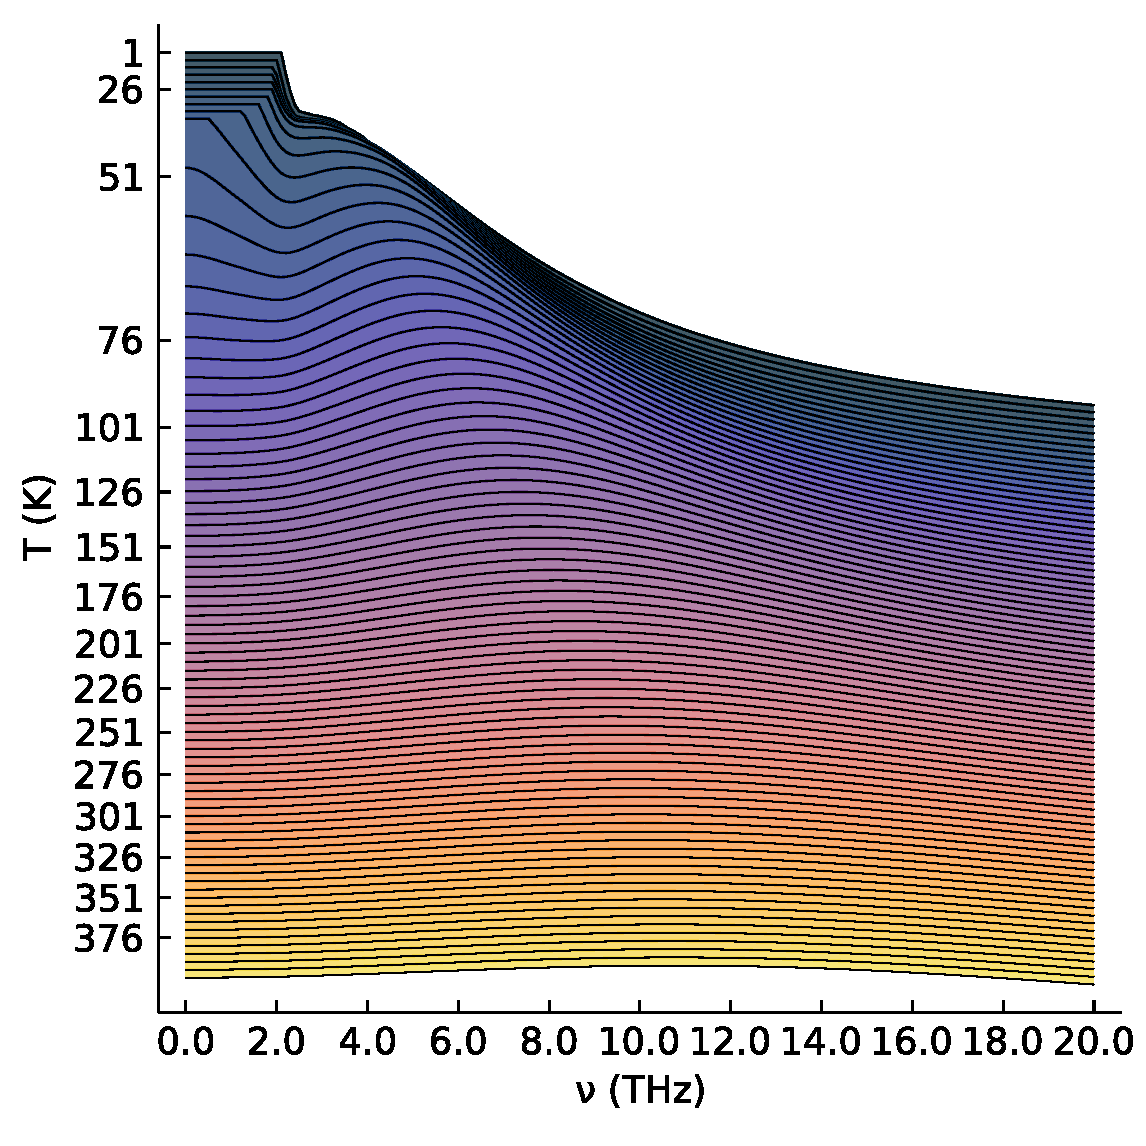
\includegraphics[width=.88\textwidth]{chapters/frohlich/figures/multi_plot_temp_abs.pdf}
\end{subfigure}%
\begin{subfigure}[t]{0.01\textwidth}
    \vspace*{-7.5cm}\textbf{f}
  \end{subfigure}%
\begin{subfigure}[b]{.58\textwidth}
\centering
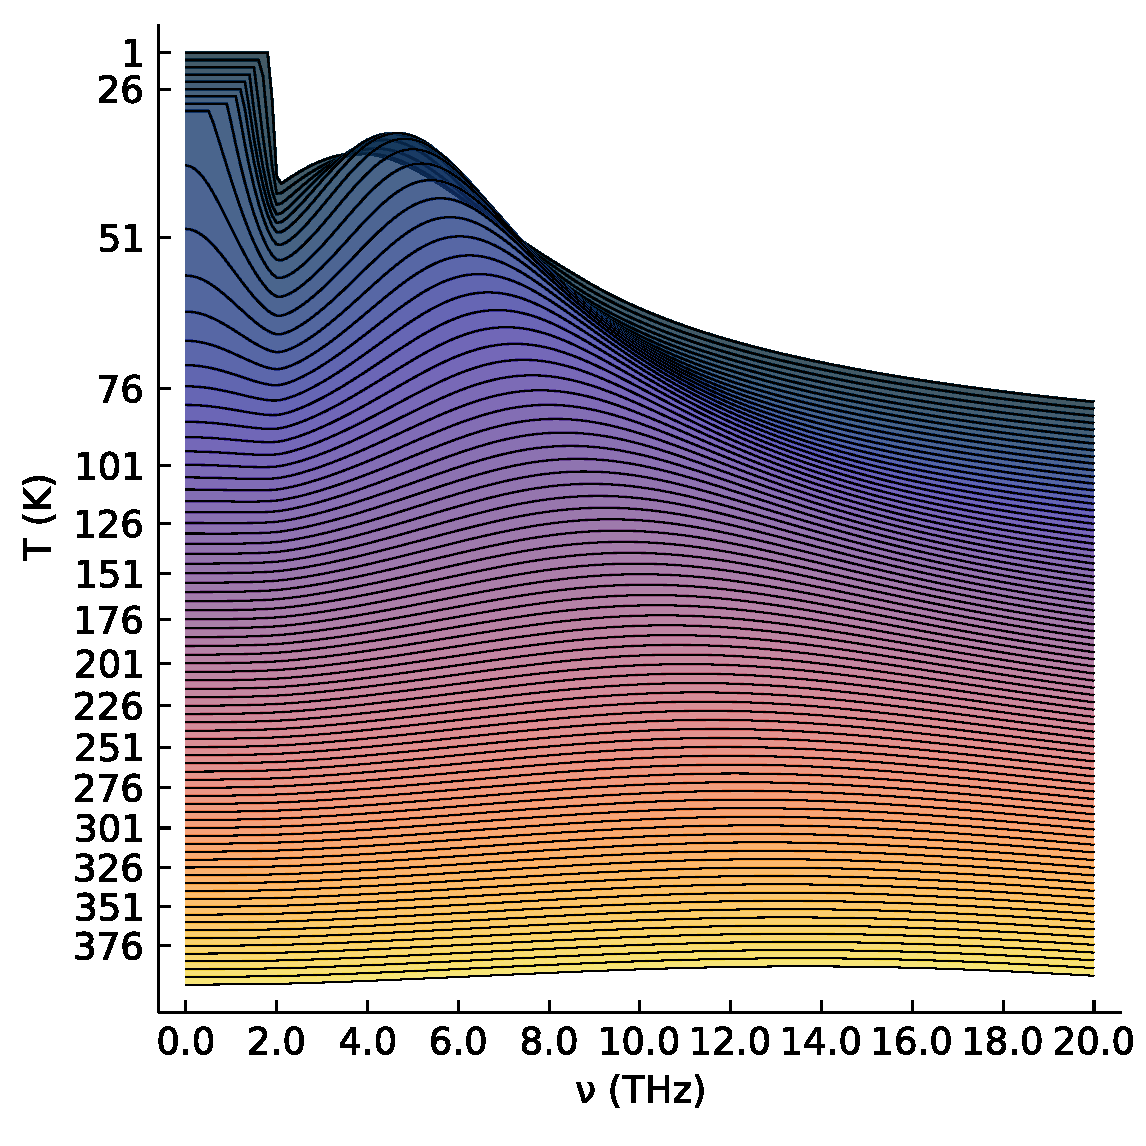
\includegraphics[width=.88\textwidth]{chapters/frohlich/figures/B_plot_temp_abs.pdf}
\end{subfigure}%
}
\caption{Left: Multiple phonon scheme (a) real conductivity, (c) imaginary conductivity, (e) absolute conductivity. Right: Hellwarth `B' scheme: (b) real conductivity, (d) imaginary conductivity, (f) absolute conductivity. At lower temperatures the conductivity has been cut-off at $600$ to enable us to see the main features.}
\label{fig:multiridge}
\end{figure}

\newpage

\begin{figure}
\vspace*{-1.5cm}\makebox[\linewidth][c]{%
\begin{subfigure}[t]{0.01\textwidth}
    \vspace*{-7.5cm}\textbf{a}
  \end{subfigure}%
\begin{subfigure}[b]{.58\textwidth}
\centering
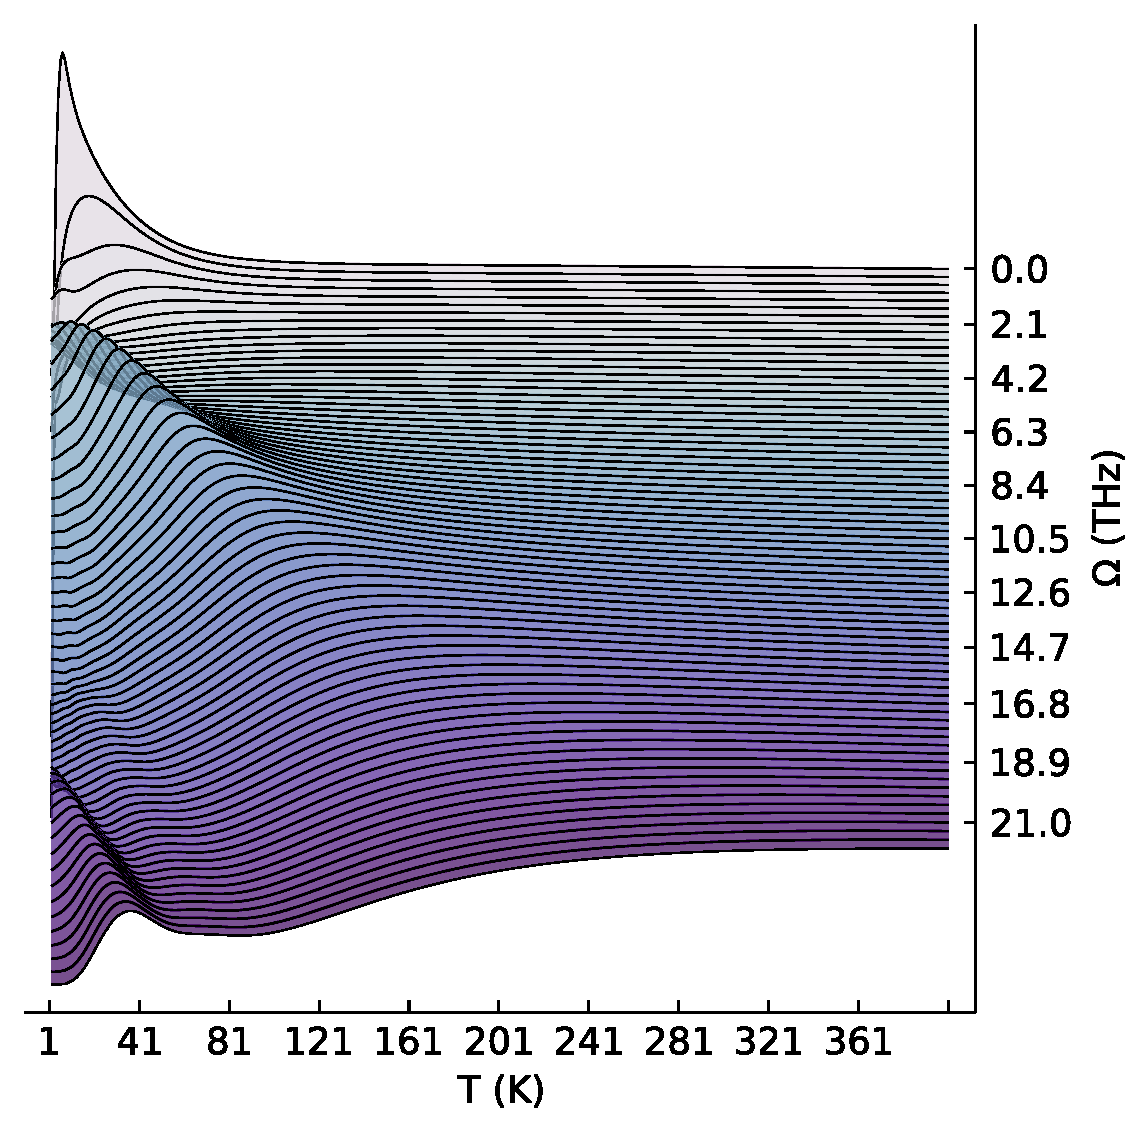
\includegraphics[width=.9\textwidth]{chapters/frohlich/figures/multi_plot_freq_real.pdf}
\end{subfigure}%
\begin{subfigure}[t]{0.01\textwidth}
    \vspace*{-7.5cm}\textbf{b}
  \end{subfigure}
\begin{subfigure}[b]{.58\textwidth}
\centering
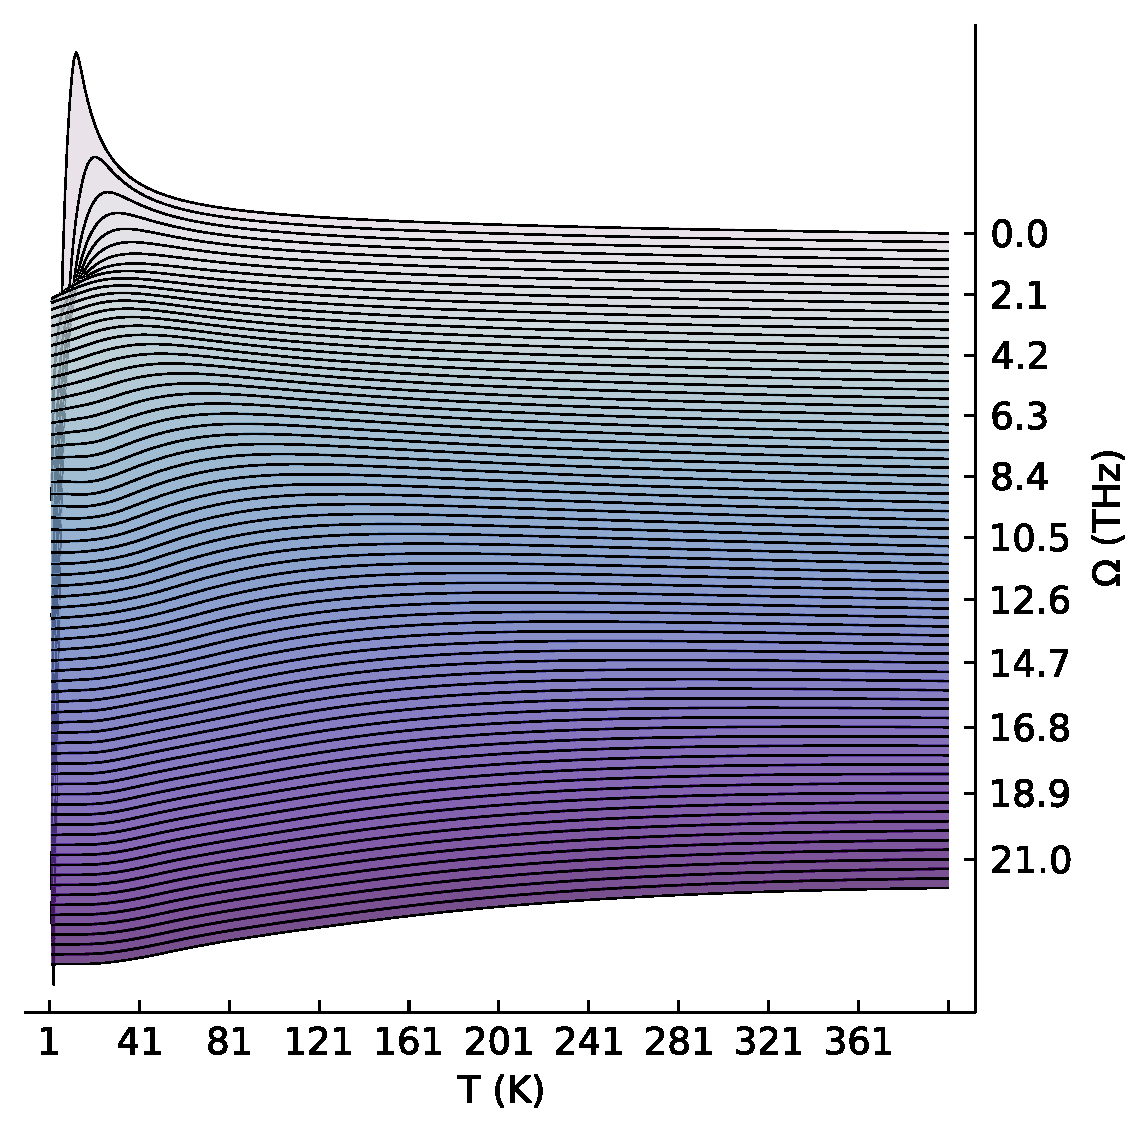
\includegraphics[width=.9\textwidth]{chapters/frohlich/figures/A_plot_freq_real.pdf}
\end{subfigure}%
}\\
\makebox[\linewidth][c]{%
\begin{subfigure}[t]{0.01\textwidth}
    \vspace*{-7.5cm}\textbf{c}
  \end{subfigure}%
\begin{subfigure}[b]{.58\textwidth}
\centering
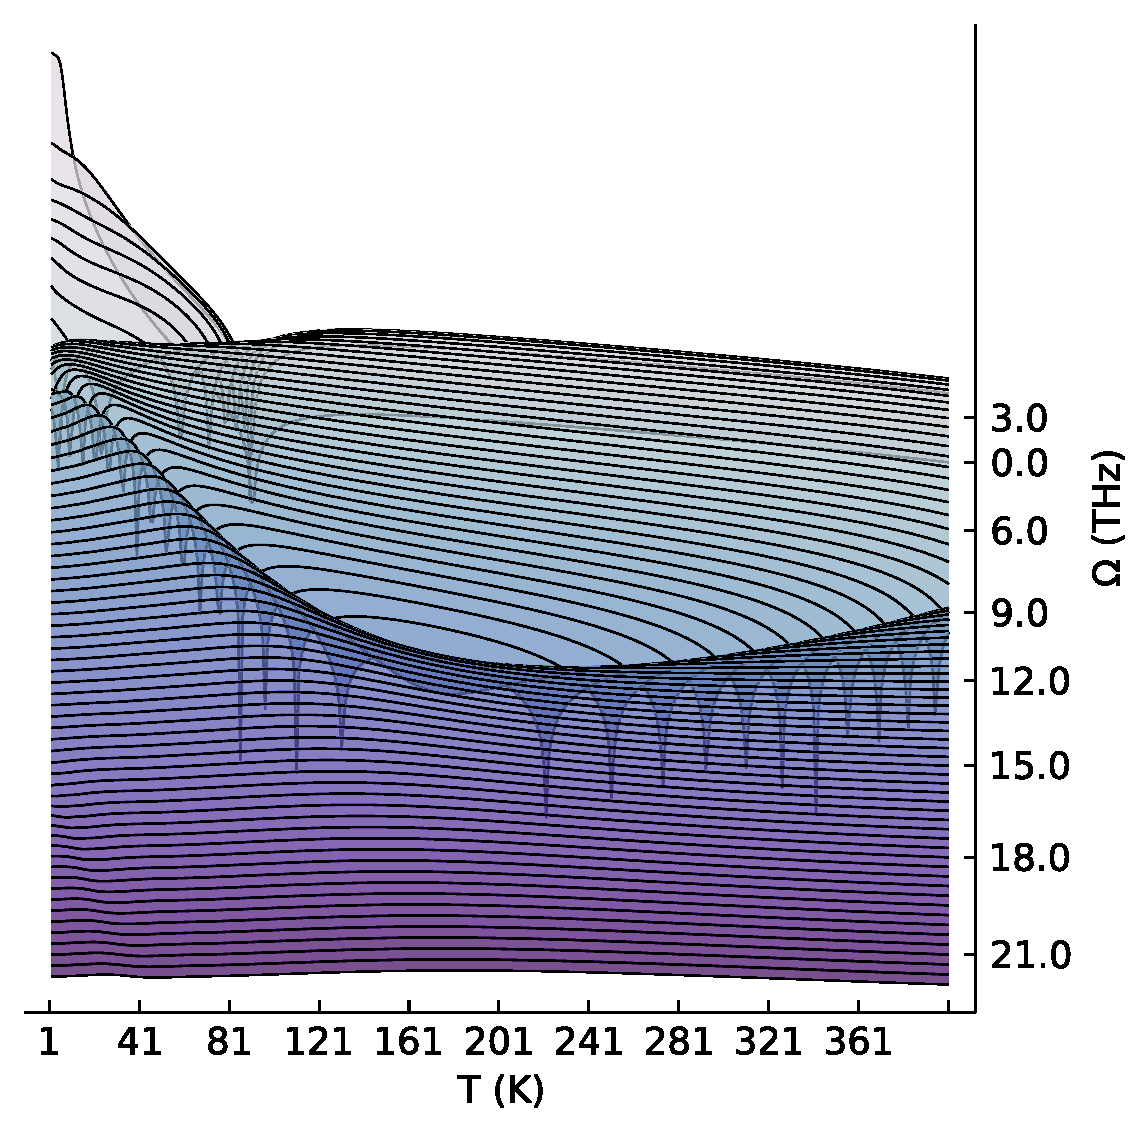
\includegraphics[width=.9\textwidth]{chapters/frohlich/figures/multi_plot_freq_imag.pdf}
\end{subfigure}%
\begin{subfigure}[t]{0.01\textwidth}
    \vspace*{-7.5cm}\textbf{d}
  \end{subfigure}%
\begin{subfigure}[b]{.58\textwidth}
\centering
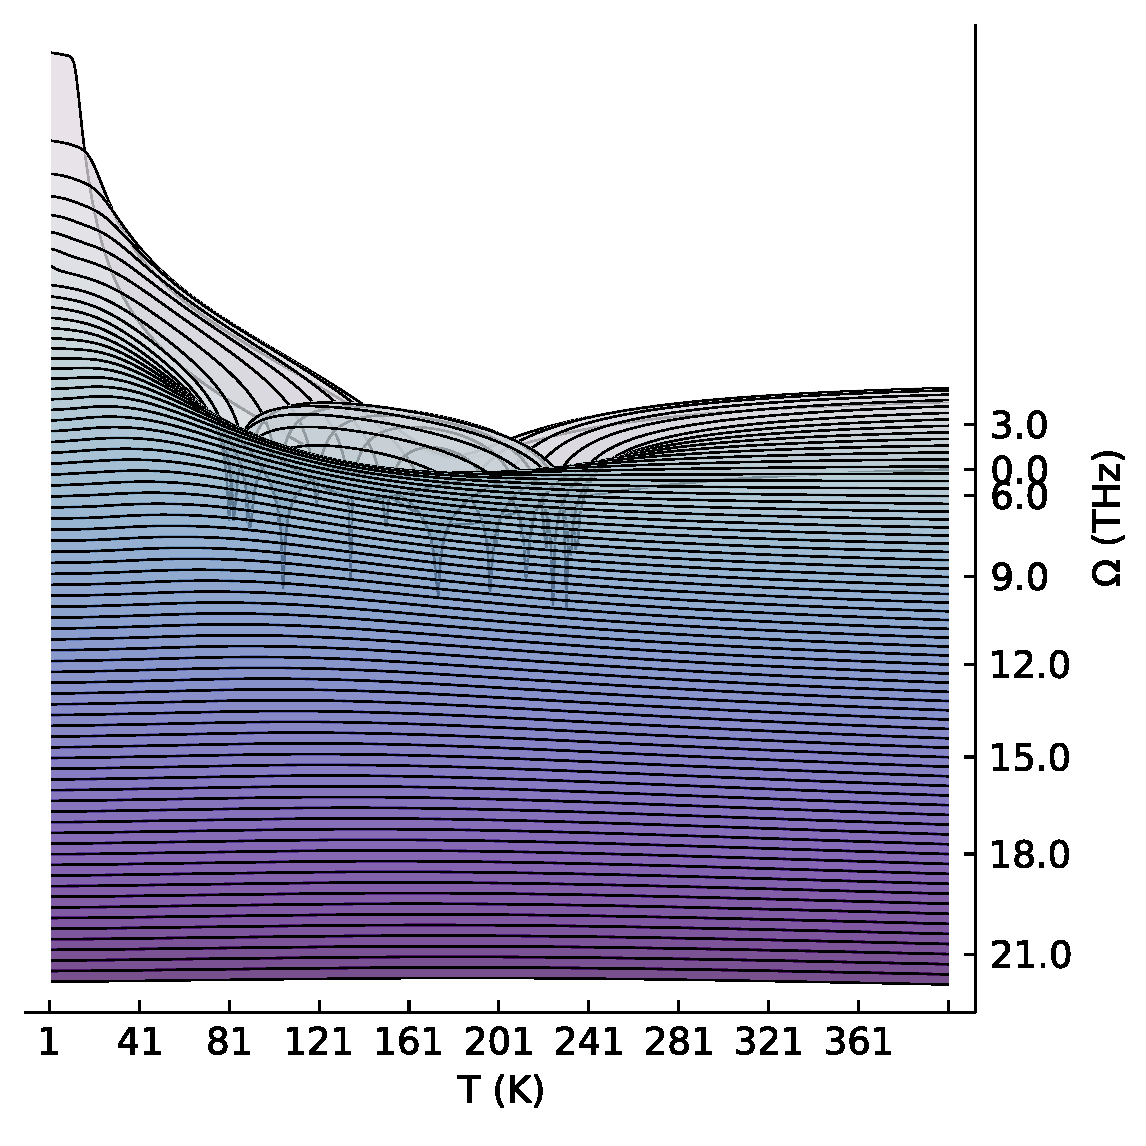
\includegraphics[width=.9\textwidth]{chapters/frohlich/figures/A_plot_freq_imag.pdf}
\end{subfigure}%
}
\makebox[\linewidth][c]{%
\begin{subfigure}[t]{0.01\textwidth}
    \vspace*{-7.5cm}\textbf{e}
  \end{subfigure}%
\begin{subfigure}[b]{.58\textwidth}
\centering
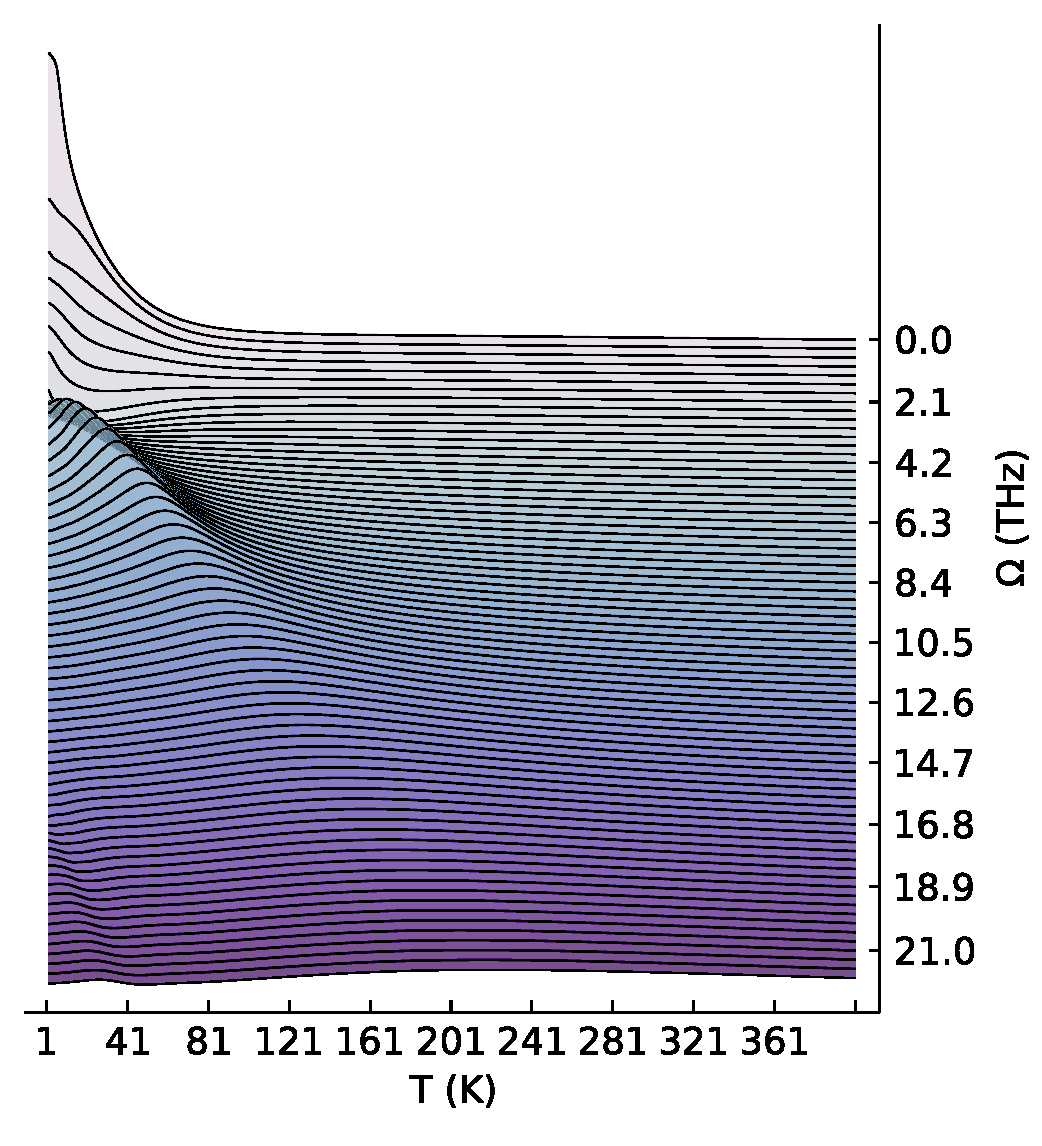
\includegraphics[width=.9\textwidth]{chapters/frohlich/figures/multi_plot_freq_abs.pdf}
\end{subfigure}%
\begin{subfigure}[t]{0.01\textwidth}
    \vspace*{-7.5cm}\textbf{f}
  \end{subfigure}%
\begin{subfigure}[b]{.58\textwidth}
\centering
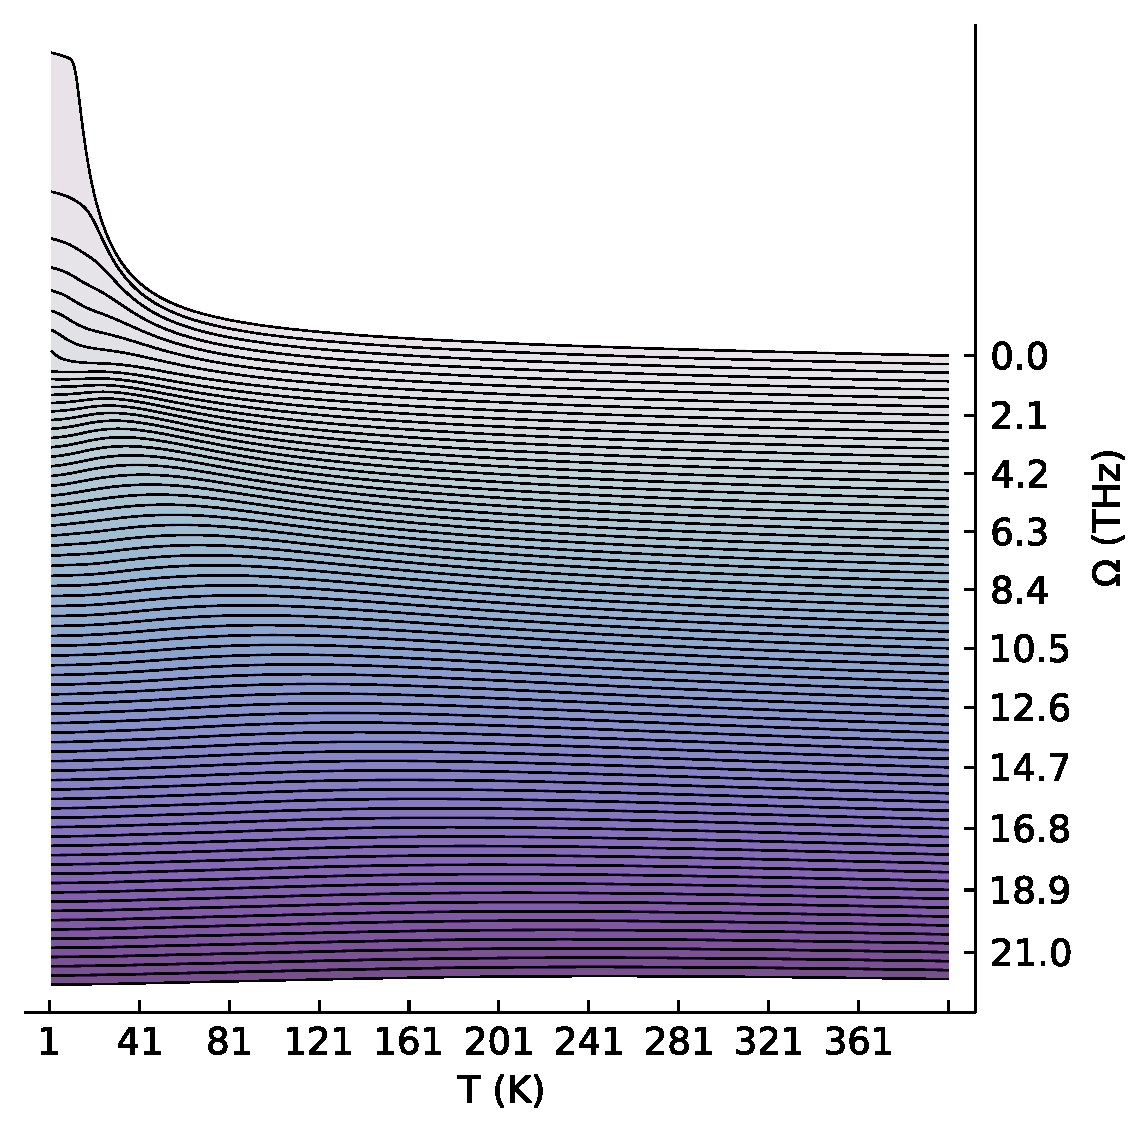
\includegraphics[width=.9\textwidth]{chapters/frohlich/figures/A_plot_freq_abs.pdf}
\end{subfigure}%
}
\caption{(a) Multiple phonon real conductivity. (b) A scheme real conductivity. (c) Multiple phonon imaginary conductivity. (d) A scheme imaginary conductivity. (e) Multiple phonon absolute conductivity. (f) A scheme absolute conductivity.}
\end{figure}

\subsection{Modelling terahertz spectroscopy unveiled polaron photoconductivity dynamics in Metal-Halide Perovskites}

\begin{figure}[t]
\makebox[\linewidth][c]{%
\begin{subfigure}[b]{.6\textwidth}
\centering
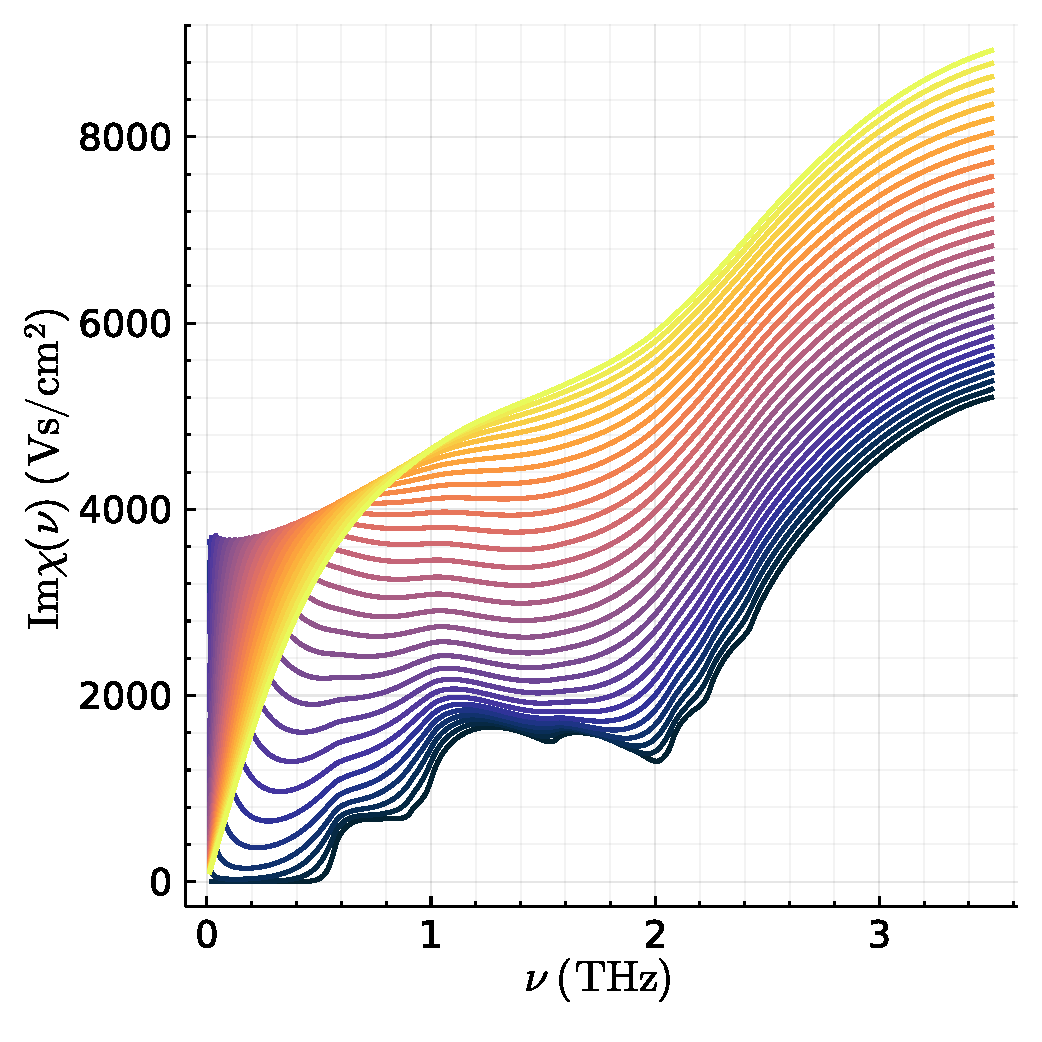
\includegraphics[width=.9\textwidth]{chapters/frohlich/figures/zero_mem.pdf}
\end{subfigure}%
\begin{subfigure}[b]{.6\textwidth}
\centering
\includegraphics[width=.9\textwidth]{chapters/frohlich/figures/zero_conduct.pdf}
\end{subfigure}%
}
\caption{(left): The imaginary part of the multiple phonon mode memory function in Eq. (\ref{eqn:multi_memory}) evaluated for MAPbI$_3$. (right): The real part of the multiple phonon mode complex conductivity (i.e. mobility) in Eq. (\ref{eqn:freq_dep_mobility}) evaluated for MAPbI$_3$. These are calculated for the phonon modes listed in Table 1. The reduced thermodynamic beta $\beta_j = \hbar \omega_j / (k_B T)$ is evaluated for temperatures $T = 1$ K (black curves) to $T = 30$ K (yellow curves).}
\label{fig:athermal_thz}
\end{figure}

Recently, we used used ultrafast visible pump-infrared push-terahertz probe spectroscopy to measure the real-time photo-conductivity of methyl-ammonium lead iodide in~\cite{zheng_multipulse_2021}. In this paper, I provided my multiple phonon mode mobility, applied to the $15$ modes of MAPbI$_3$ in Table 1, to model the complex conductivity and compare the results to the photo-conductivity measurements. 

\begin{figure}[t]
\makebox[\linewidth][c]{%
\begin{subfigure}[b]{.6\textwidth}
\centering
\includegraphics[width=1\textwidth]{chapters/frohlich/figures/thz_plot.pdf}
\end{subfigure}
}
\caption{Terahertz photo-conductivity spectra obtained from a visible pump-IR push-THz probe measurement in~\cite{zheng_multipulse_2021}. The plot shows the real (solid markers) and imaginary (hollow markers) parts of the complex conductivity in MAPbI$_3$. The blue, black and green dashed-lines show before, at and after the arrival of the push pulse, respectively.}
\label{fig:thzplot}
\end{figure}

In Figure \ref{fig:athermal_thz} I provide the low-temperature ($T = 1$ 
K to $T = 30$ K) results of the imaginary component of the memory function $\text{Im}\chi(\nu)$ (left) and the real part of the complex conductivity $\text{Re}\sigma(\nu)$ (right). These have peaks that occur around the frequencies $0.60$ THz, $1.25$ THz and $1.75$ THz, as well as a very broad peak that starts around $2.00$ THz that seems to have extra peaks underlying it to give the appearance of oscillations around $2.15$ THz and $2.25$ THz. 

From Figures \ref{fig:multicontour} and \ref{fig:multiridge} we see that the broad peak is the last feature which decays away at higher frequencies. The broad peak has a maximum around $3.00$ THz at $T = 1$, which flattens and shifts to higher frequencies at higher temperatures where it becomes the only remaining feature. This is to be compared to the photo-conductivity measurements shown in Figure \ref{fig:thzplot}, where the real component maxima occur around the frequencies $1.25$ THz and $2.25$ THz, with a shoulder occur on the side of the $1.25$ THz peak around $0.60$ THz. The shoulder and $1.25$ THz peak seem to be in agreement with the multiple phonon model, however the broader peak, whilst roughly around the right frequency of $2.25$ THz, is far broader and prominent in the theoretical model compared to the photo-conductivity measurements. 

One thing to note is the apparent temperature differences between the multiple phonon model and the experiment. In the multiple phonon model, the one-phonon peaks associated with each phonon mode only appear at very low-temperatures and are quickly washed out as the temperature increases until at around $T > 10$ K, only the broad peak around $3.00$ Thz remains. In the multiple phonon theory, it is assumed that the electron and phonon thermal-bath are at thermal equilibrium. However, in the experiment the electron(s) is definitely not at thermal equilibrium and is very hot.

\begin{figure}[h]
\makebox[\linewidth][c]{%
\begin{subfigure}[b]{.6\textwidth}
\centering
\includegraphics[width=.9\textwidth]{chapters/frohlich/figures/multi_contour_real_chi.pdf}
\end{subfigure}%
\begin{subfigure}[b]{.6\textwidth}
\centering
\includegraphics[width=.9\textwidth]{chapters/frohlich/figures/multi_contour_real_0.pdf}
\end{subfigure}%
}
\caption{Contour plots for (left): The imaginary part of the multiple phonon mode memory function (\ref{eqn:multi_memory}) evaluated for MAPbI$_3$. (right): The real part of the multiple phonon mode complex conductivity (\ref{eqn:freq_dep_mobility}) evaluated for MAPbI$_3$. Here the temperature axis is log-scaled and ranges from $T = 1$ K to $T = 400$ K and frequency zoomed in onto the range $\nu = 0$ THz to $\nu = 3.5$ THz.}
\label{fig:thermal_thz}
\end{figure}

\begin{figure}[t]
\makebox[\linewidth][c]{%
\begin{subfigure}[b]{.6\textwidth}
\centering
\includegraphics[width=.9\textwidth]{chapters/frohlich/figures/ff_zpr.pdf}
\end{subfigure}%
\begin{subfigure}[b]{.6\textwidth}
\centering
\includegraphics[width=.9\textwidth]{chapters/frohlich/figures/ff_emass.pdf}
\end{subfigure}%
}
\caption{Both figures are taken from~\cite{guster_frohlich_2021}. (left): The relative differences between the ground-state energy of the polaron determined using perturbation theory (which fully accounts for any anisotropy) and the Feynman variational approach (using my approximate treatment of anisotropy). (right): The relative difference between the effective masses determined using perturbation theory and the Feynman variational approach (again only approximately accounting for anisotropy). $m^*_{P, iso}$ is the isotropic effective mass, $m^*_{P, \perp}$ and $m^*_{P, z}$ are the in-plane and out-of-plane polaron effective masses.}
\label{fig:anisotropy}
\end{figure}

\section{Fr\"ohlich polaron effective mass and localisation length in cubic materials:  degenerate and anisotropic electronic bands}

In~\cite{guster_frohlich_2021}, we investigate the polaron effective mass, radius and ground-state energy that arise from a generalised Fr\"ohlich Hamiltonian that incorporates degenerate bands with anisotropy and multiple phonon branches. These polaron properties are calculated for 20 cubic materials (including II-VI compounds: CdS, CdSe, CdTe, ZnS, ZnSe, ZnTe; III-V compounds: AlAs, AlSb, AlP, BAs, BN, GaAs, GaN, GaP; oxides: BaO, CaO, Li$_2$O, MgO, SrO; and SiC) using the lowest order of perturbation theory and the strong coupling limit. \newline

\noindent In the non-degenerate case, I provide a na\"ive extension of Feynman's path integral approach to include anisotropic effective band masses which is used as a point of comparison with the full perturbative treatment for characterising the polaron in the weak-coupling limit (c.f. section IIb in~\cite{guster_frohlich_2021} and subsection 3.8 of this chapter). From Figure \ref{fig:anisotropy} (left) we see that the variational approach gives a lower estimate for the ground-state compared to the perturbative result for both isotropic (up to $2.5$\% lower) and anisotropic (up to $17.5$\% lower) materials. In Figure \ref{fig:anisotropy} (right), we have the relative difference in polaron effective mass between the two approaches. The largest difference is found in materials that, within the Fr\"ohlich approach, are found in~\cite{guster_frohlich_2021} to be at the continuum limit breakdown where the discrete nature of the lattice cannot be ignored. These materials include BaO, CaO, SrO and, to a lesser extent, Li$_2$O. In both the anisostropic and isotropic cases the relative difference increases with polaron effective mass, and the in-plane and out-of-plane effective mass differences seem to diverge. This sudden increase in the relative difference is associated with a breakdown limit around $\alpha = 6$ in the perturbative approach for determining the polaron effective mass.

\section{Variational Holstein Polaron}

\subsection{Coupling Dependence}

The main weak-to-strong polaron transition to occurs around $\alpha^{{H}} \approx 2$ for the Holstein model when using Stefano's convention. Elsewhere in the literature this is happens at $\alpha^{(H)} \approx 1$ or at some other value. Ultimately, this is just a matter of re-scaling the Holstein alpha parameter. I have assumed that this polaron transition is similar in nature to the $\alpha = 6$ transition present in the Fr\"ohlich model - where perturbation theory diverges. Therefore, whenever I am comparing the Holstein polaron results to the Fr\"ohlich polaron, I will  the Fr\"ohlich alpha according to a rough expression
\begin{equation}
    \alpha^{(F)} \approx 3 \alpha^{(H)}
\end{equation}
This expression has only be deduced by eye and is not mathematically derived, but it will allow us to (I hope) better compare the Fr\"ohlich and Holstein models and differentiated their underlying physics. I choose to scale the Fr\"ohlich model so that direct comparison with diagMC results is maintained and to avoid any possible unforeseen complications on the Holstein variational solution.

\subsubsection{Polaron Ground-state Energy}

\begin{figure}
  \begin{subfigure}[b]{0.49\textwidth}
    \includegraphics[width=\textwidth]{figures/energy_alpha_fro.png}
  \end{subfigure}
  \hfill
  \begin{subfigure}[b]{0.49\textwidth}
    \includegraphics[width=\textwidth]{figures/energy_alpha.png}
  \end{subfigure}
  \caption{Polaron binding energy for the Fr\"ohlich and Holstein models with respect to the electron-phonon dimensionless coupling parameter $\alpha$. \textbf{Left:} Fr\"ohlich model in 2D (solid blue) and 3D (dashed orange). \textbf{Right:} Holstein model in 1D (dashed orange), 2D (dot-dashed green) and 3D (dot-dot-dashed pink), and the 3D Fr\"ohlich result scaled by $1/6$ in energy and $1/3$ in $\alpha$ to align with the Holstein weak-coupling ($\alpha < 1$). Co-plotted are DiagMC results for the Holstein model in 1D (blue diamonds), 2D (orange squares) and 3D (green circles).}
  \label{fig:energy_alpha}
\end{figure}

The first numerical result in Fig. (\ref{fig:energy_alpha}) is the dependence on the Holstein free energy on the unitless alpha parameter $\alpha$. On the left we have the Fr\"ohlich free energy for 2D and 3D and on the right we have the Holstein free energy compared to diagMC data in 1D, 2D and 3D. The predictions made by this new variational theory agree fairly well with the diagMC, especially prior to the transition point at $\alpha = 2$ which is characterised by a distinctive kink in the free energy. After $\alpha = 2$, the variational theory \emph{underestimates} the true free energy. Now, this begs an important question: is this theory actually variational? From its construction, it should \emph{only} ever provide an $\textbf{upper-bound}$ to the polaron free energy, so at first sight it going below the diagMC data is concerning. However, it should be recognise that in order to apply the variational approximation we have to approximate the Holstein model electron band as an unbounded parabola. Therefore, the variational method inevitably overestimates the kinetic energy in the model, which should asymptotic to zero at large coupling. However, in our model, it continues to grow rough as $KE \sim \sqrt{\alpha}$. So, I argue that the variational bound is preserved, we're just not solving for the Holstein model exactly due to the approximations made along the way. Nonetheless, the variational approximation seems to capture the same small polaron transition at $\alpha = 2$ remarkably well as having the correct dependence and scaling with the number of spatial dimensions.
\newline

On another note, the Holstein model has a free energy that is significantly smaller than the large Fr\"ohlich polaron. On the right we have co-plotted the 3D Fr\"ohlich free energy result in pink, scaled down by a factor of $6$ to bring it inline with the weak-coupling prediction of the Holstein model. This suggests that polaronic effects are stronger in materials that can form large polarons. Conceptually this is logical as the Holstein electron-phonon interaction is purely local and isolated to individual lattice sites, whereas in the Fr\"ohlich model it is a long-range interaction and thus more strongly bounding.

\subsubsection{Polaron Variational Parameters}

\begin{figure}
  \begin{subfigure}[b]{0.49\textwidth}
    \includegraphics[width=\textwidth]{figures/vw_alpha_fro.png}
  \end{subfigure}
  \hfill
  \begin{subfigure}[b]{0.49\textwidth}
    \includegraphics[width=\textwidth]{figures/vw_alpha_hol.png}
  \end{subfigure}
  \caption{Optimal values of the polaron variational parameters $v$ and $w$ for the Fr\"ohlich and Holstein models with respect to the electron-phonon dimensionless coupling parameter $\alpha$. \textbf{Left:} Fr\"ohlich model in 2D ($v$ solid blue and $w$ dot-dash green) and 3D ($v$ dashed orange and $w$ dot-dot-dash pink). \textbf{Right:} Holstein model in 1D ($v$ solid blue and $w$ dot-dot-dash pink), 2D ($v$ dashed orange and $w$ solid yellow) and 3D ($v$ dot-dashed green and $w$ dashed turquoise).}
  \label{fig:vw_alpha}
\end{figure}

Next are the results for the $v$ and $w$ variational parameters for the Holstein model (Fig. (\ref{fig:vw_alpha})). On the left we have the Fr\"ohlich results in 2D and 3D. On the right we have the Holstein results in 1D, 2D and 3D. We assume that the alpha ranges used produce similar physical regimes within either model for point of comparison, as mentioned above.
\newline

Immediately, the Holstein model noticeably has a very different variational solution to the Fr\"ohlich model which a distinctive discontinuity around $\alpha = 2$ which causes a suddenly more rapid increase in the polaron binding energy. This is attributed to transitioning into a small polaron state. Both models have $w \to 1 \omega_0$ at large coupling, albeit more abruptly in the Holstein model. Also, the $v$ parameters appear to have a different strong coupling dependency on $\alpha$. In the Fr\"ohlich model at large $\alpha$, $v^{(F)} \sim \alpha^2$ whereas in the Holstein model $v^{(H)} \sim \sqrt{\alpha}$. Another noticeable difference is in the $\alpha \to 0$ limits where regardless of the number of spatial dimensions, the Fr\"ohlich model parameters asymptote to $v = w = 3$, but in the Holstein model the zero-coupling limit depends on the number of spatial dimensions. Finally, the polaron transition seems to be dimensionally-dependent in the Fr\"ohlich model, occuring at $\alpha = \approx 3$ in 2D and $\alpha \approx 6$ in 3D. Whereas the transition in the Holstein model seems to be independent on the dimensionality. It should be noted however, that the alpha unitless coupling is often \emph{defined} this way.

\subsection{Holstein Polaron Temperature Dependence}

In this section we look at how the Holstein model varies with temperature. Notably, its free energy, variational parameters and DC mobility. As the $v$ and $w$ parameter scale to large values with temperature, I have opted to represent them in terms of the trial model fictitious particle mass $M = v^2 / w^2 - 1$ and spring-constant $\kappa = v^2 - w^2$ instead as they produce more readable and digestible plots. The temperature range looked at is $T = 0.125 \omega_0$ to $T = 32 \omega_0$. For clearer context, in the Fr\"ohlich model, $T = \omega_0$ is roughly $T \approx 48 $K
and in the Holstein model it is roughly $T \approx 11.6 $K up to a multiple of the phonon frequency in units of THz$2\pi$. We also look at these temperature over a range of couplings $\alpha^{(F)} = 2.5, 4, 6, 8, 10, 12$ and $\alpha^{(H)} \approx \alpha^{(F)} / 3 = 0.83, 1.33, 2, 2.67, 3.33, 4$.

\subsubsection{Holstein Polaron Free Energy}

\begin{figure}[!tbp]
  \begin{subfigure}[b]{0.49\textwidth}
    \includegraphics[width=\textwidth]{figures/energy_temp_25_083.png}
  \end{subfigure}
  \hfill
  \begin{subfigure}[b]{0.49\textwidth}
    \includegraphics[width=\textwidth]{figures/energy_temp_4_133.png}
  \end{subfigure}
  \begin{subfigure}[b]{0.49\textwidth}
    \includegraphics[width=\textwidth]{figures/energy_temp_6_2.png}
  \end{subfigure}
  \hfill
  \begin{subfigure}[b]{0.49\textwidth}
    \includegraphics[width=\textwidth]{figures/energy_temp_8_267.png}
  \end{subfigure}
  \begin{subfigure}[b]{0.49\textwidth}
    \includegraphics[width=\textwidth]{figures/energy_temp_10_333.png}
  \end{subfigure}
  \hfill
  \begin{subfigure}[b]{0.49\textwidth}
    \includegraphics[width=\textwidth]{figures/energy_temp_12_4.png}
  \end{subfigure}
  \caption{Polaron binding energy for the Fr\"ohlich model in 2D (dot-dash pink) and 3D (solid gold), and Holstein model in 1D (solid blue), 2D (dashed orange) and 3D (dotted green) with respect to temperature (in units of the phonon frequency $\omega_0$), for values of the Fr\"ohlich electron-phonon coupling $\alpha = 2.5, 4, 6, 8, 10, 12$ and $1/3$ of these values for the Holstein electron-phonon coupling. The Fr\"ohlich free energy has been scaled down by $1/6$ to better compare with the Holstein free energy.}
  \label{fig:energy_temp}
\end{figure}

In Figs. (\ref{fig:energy_temp}) we have many plots showing how the temperature dependence of the Holstein polaron in 1D, 2D and 3D, and the Fr\"ohlich polaron in 2D and 3D, changes as the electron-phonon coupling increases. Note that the Fr\"ohlich free energy has been scaled down by $1/6$ to better compare trends with the Holstein free energy. A few trends can be noticed. First and foremost, at weaker coupling ($\alpha^{(F)} = 2.5$, $\alpha^{(H)} = 0.83$) the Holstein polaron energy grows more rapidly with increasing temperature than the Fr\"ohlich polaron, but this difference fades with increasing coupling until they seem to have a similar dependence on temperature. Secondly, the different dimensional Holstein polarons have a similar temperature dependence at all coupling, aside from a seemingly constant multiplicative factor where the 1D and 2D Holstein polaron energies are roughly $1/3$ and $2/3$ respectively of the 3D Holstein polaron. 

\subsubsection{Polaron Mass and Spring Constant}

\begin{figure}[!tbp]
  \begin{subfigure}[b]{0.49\textwidth}
    \includegraphics[width=\textwidth]{figures/mass_temp_25_083.png}
  \end{subfigure}
  \hfill
  \begin{subfigure}[b]{0.49\textwidth}
    \includegraphics[width=\textwidth]{figures/mass_temp_4_133.png}
  \end{subfigure}
  \begin{subfigure}[b]{0.49\textwidth}
    \includegraphics[width=\textwidth]{figures/mass_temp_6_2.png}
  \end{subfigure}
  \hfill
  \begin{subfigure}[b]{0.49\textwidth}
    \includegraphics[width=\textwidth]{figures/mass_temp_8_267.png}
  \end{subfigure}
  \begin{subfigure}[b]{0.49\textwidth}
    \includegraphics[width=\textwidth]{figures/mass_temp_10_333.png}
  \end{subfigure}
  \hfill
  \begin{subfigure}[b]{0.49\textwidth}
    \includegraphics[width=\textwidth]{figures/mass_temp_12_4.png}
  \end{subfigure}
  \caption{Temperature dependence ($T$, in units of phonon frequency $\omega_0$) of the fictitious particle mass $M$ from the trial system for the Fr\"ohlich model in 2D (solid blue) and 3D (dashed orange), and for the Holstein model in 1D (dot-dashed green), 2D (dot-dot-dashed pink) and 3D (solid gold), for values of the Fr\"ohlich electron-phonon coupling $\alpha = 2.5, 4, 6, 8, 10, 12$ and $1/3$ of these values for the Holstein electron-phonon coupling. This mass can be express in terms of the traditional $v$ and $w$ using $M = (v^2 - w^2) / w^2$. The Fr\"ohlich results are un-scaled here.}
  \label{fig:mass_temp}
\end{figure}

\begin{figure}[!tbp]
  \begin{subfigure}[b]{0.49\textwidth}
    \includegraphics[width=\textwidth]{figures/spring_temp_25_083.png}
  \end{subfigure}
  \hfill
  \begin{subfigure}[b]{0.49\textwidth}
    \includegraphics[width=\textwidth]{figures/spring_temp_4_133.png}
  \end{subfigure}
  \begin{subfigure}[b]{0.49\textwidth}
    \includegraphics[width=\textwidth]{figures/spring_temp_6_2.png}
  \end{subfigure}
  \hfill
  \begin{subfigure}[b]{0.49\textwidth}
    \includegraphics[width=\textwidth]{figures/spring_temp_8_267.png}
  \end{subfigure}
  \begin{subfigure}[b]{0.49\textwidth}
    \includegraphics[width=\textwidth]{figures/spring_temp_10_333.png}
  \end{subfigure}
  \hfill
  \begin{subfigure}[b]{0.49\textwidth}
    \includegraphics[width=\textwidth]{figures/spring_temp_12_4.png}
  \end{subfigure}
  \caption{Temperature dependence ($T$, in units of phonon frequency $\omega_0$) of the fictitious particle spring-constant $\kappa$ from the trial system for the Fr\"ohlich model in 2D (solid blue) and 3D (dashed orange), and for the Holstein model in 1D (dot-dashed green), 2D (dot-dot-dashed pink) and 3D (solid gold), for values of the Fr\"ohlich electron-phonon coupling $\alpha = 2.5, 4, 6, 8, 10, 12$ and $1/3$ of these values for the Holstein electron-phonon coupling. This mass can be express in terms of the traditional $v$ and $w$ using $\kappa = (v^2 - w^2)$. The Fr\"ohlich results are un-scaled here.}
  \label{fig:spring_temp}
\end{figure}

In Figs. (\ref{fig:mass_temp}) we have the temperature dependence of the fictitious particle mass for the Holstein polaron with varying electron-phonon coupling. At smaller coupling both the Holstein and Fr\"ohlich models show a maximum at intermediate temperatures and show similar dependence on temperature up until some critical transition temperature where the Holstein polaron mass abruptly stops decreasing with temperature and starts to become heavier, unlike the Fr\"ohlich polaron mass which continues to get lighter with increasing temperatures until reducing tot he electron band-mass at infinite temperature. At stronger coupling, the maximum mass at intermediate temperatures and is replaced with a plateaued maximum that exists for all temperature $T < \omega_0$. The critical transition temperature at higher temperature still exists for the Holstein polaron mass.
\newline

The plateau less than the phonon energy $T < \omega_0$ arises due to the lack of excited phonons whose random motion leads to a decrease of the effective electron-phonon interaction which results in a decreasing phonon contribution to the effective electron 
mass. For the Holstein model the polaron mass starts to increase at a critical temperature equal to the natural frequency of the electron-phonon interaction $v$. Phonons then begin to transfer energy back into the effective electron-phonon interaction and increasing the phonon contribution to the effective electron mass.
\newline

In Figs. (\ref{fig:spring_temp}) we have the temperature dependence of the fictitious particle spring constant for the Holstein polaron with varying electron-phonon coupling. An interesting difference here is that the spring-constant for the Fr\"ohlich polaron keeps increasing linearly with temperature whereas the spring-constant for the Holstein polaron seems to plateau to some value at higher temperatures. This is most noticeable at weaker couplings. Similar to the polaron mass, as we go to stronger coupling both kinds of polarons reach a constant spring-constant for temperatures lower than than the phonon energy.
\newline

One final overall observation is that the 2D Holstein polaron and the 3D Fr\"ohlich polaron seem to be most similar. This isn't all that surprising, since it only for two dimensions that the self-interaction functional (Eqn. \ref{eqn:general_self_interaction})) in the Holstein model has the same phonon-momentum dependence as in the Fr\"ohlich model - which does not change with dimensionality unlike for the Holstein polaron.

\subsubsection{Polaron Mobility}

\begin{figure}[!tbp]
  \begin{subfigure}[b]{0.49\textwidth}
    \includegraphics[width=\textwidth]{figures/mobility_temp_25_083.png}
  \end{subfigure}
  \hfill
  \begin{subfigure}[b]{0.49\textwidth}
    \includegraphics[width=\textwidth]{figures/mobility_temp_4_133.png}
  \end{subfigure}
  \begin{subfigure}[b]{0.49\textwidth}
    \includegraphics[width=\textwidth]{figures/mobility_temp_6_2.png}
  \end{subfigure}
  \hfill
  \begin{subfigure}[b]{0.49\textwidth}
    \includegraphics[width=\textwidth]{figures/mobility_temp_8_267.png}
  \end{subfigure}
  \begin{subfigure}[b]{0.49\textwidth}
    \includegraphics[width=\textwidth]{figures/mobility_temp_10_333.png}
  \end{subfigure}
  \hfill
  \begin{subfigure}[b]{0.49\textwidth}
    \includegraphics[width=\textwidth]{figures/mobility_temp_12_4.png}
  \end{subfigure}
  \caption{Temperature dependence ($T$, in units of phonon frequency $\omega_0$) of the polaron DC mobility $\mu$ for the Fr\"ohlich model in 2D (solid blue) and 3D (dashed orange), and for the Holstein model in 1D (dot-dashed green), 2D (dot-dot-dashed pink) and 3D (solid gold), for values of the Fr\"ohlich electron-phonon coupling $\alpha = 2.5, 4, 6, 8, 10, 12$ and $1/3$ of these values for the Holstein electron-phonon coupling.}
  \label{fig:mobility_temp}
\end{figure}

In Figs. (\ref{fig:mobility_temp}) we have the temperature dependence of the polaron mobility for the Holstein polaron with varying electron-phonon coupling. At weaker coupling the mobility shows the typical exponentially decreasing band-like transport for temperatures below the phonon energy. Above the phonon energy the temperature dependence transitions to a power-law relationship $T^{-x}$ where $x$ is some number that is typically use to determine the dominant scattering mechanism within a material. For example, for acoustic phonons this index is typically $x = 3/2$. 
\newline

Again as we saw previously, 2D Holstein and 3D Fr\"ohlich appear to be most alike. As the electron-phonon coupling increases, we begin to see the onset of the ski-slope feature where the mobility takes on a local minimum at the phonon energy $T = \omega_0$ before increasing to a local maximum at the polaron quasiparticle frequency $v$ and then transitioning back into a power-law relationship at higher temperatures. Each of the different dimensions of both polaron models seem to have a different dependence on the strength of the electron-phonon coupling when it comes to the mobility. For the Fr\"ohlich polaron the ski-slope appears sooner for the 2D model than the 3D model. For the Holstein polaron the opposite trend seems to be true, with the higher dimension model exhibiting the ski-slope. The 2D Fr\"ohlich polaron also seems to manifest a low temperature maximum at larger electron-phonon couplings which transitions in a linear decrease to some finite value in mobility as the temperature goes to zero.
\newline

At high temperature the Fr\"ohlich polaron mobility follows the temperature power-law $\mu^{(H)} \sim T^{-1/2}$ which is consistent with mobility derived from the electron scattering with optical phonons. However, at high temperature the Holstein polaron mobility becomes a constant; independent of temperature. This may be attributed to the phonon-induced electron hopping between lattice-sites along which the electron motion is coherent in the direction of that particular energy band. Likewise, at low temperature the mobility increases abruptly below the Debye temperature due to the increasing contribution of the electron transfer without phonon participation.

\subsection{Frequency Dependence}

In this section we look at how the Holstein model varies with the frequency of an external, perturbing, varying electric field. Specifically, the polaron memory function which we compare to the Fr\"ohlich polaron results of FHIP \cite{Feynman1962}, and the optical conductivity which we compare to the Fr\"ohlich polaron results of DSG \cite{Devreese1972}. For the memory function we look at frequencies $\Omega / \omega_0$ from $0$ to $28$ and $\alpha^{(F)} = 3, 5, 7$ or $\alpha^{(H)} = 1, 1.67, 2.33$. For the optical conductivity we look at frequencies $\Omega / \omega_0$ from $0$ to $11$ for $\alpha^{(F)} = 1, 3, 5, 6$ or $\alpha^{(H)} = 0.33, 1, 1.67, 2$ and frequencies $\Omega / \omega_0$ from $0$ to $22$ for $\alpha^{(F)} = 7$ or $\alpha^{(H)} = 2.33$. 

\subsubsection{Polaron Memory Function}

\begin{figure}
\centering
  \begin{subfigure}[b]{0.49\textwidth}
    \includegraphics[width=\textwidth]{figures/im_mem_freq_3_1.png}
  \end{subfigure}
  \hfill
  \begin{subfigure}[b]{0.49\textwidth}
    \includegraphics[width=\textwidth]{figures/im_mem_freq_5_167.png}
  \end{subfigure}
  \begin{subfigure}[b]{0.49\textwidth}
    \centering
    \includegraphics[width=\textwidth]{figures/im_mem_freq_7_233.png}
  \end{subfigure}
  \caption{Frequency dependence ($\Omega$, in units of the phonon frequency $\omega_0$) of the polaron memory function $\chi(\Omega)$ for the Fr\"ohlich model in 3D (solid blue), and for the Holstein model in 1D (dashed orange), 2D (dot-dashed green) and 3D (solid gold), for values of the Fr\"ohlich electron-phonon coupling $\alpha = 1, 3, 5,6, 7$ and $1/3$ of these values for the Holstein electron-phonon coupling. Here I only consider the imaginary component to reduce graph clutter, but the real component was also evaluated.} 
  \label{fig:im_mem_freq}
\end{figure}

In Figs. (\ref{fig:im_mem_freq}) is the frequency-dependent imaginary component of the memory function for the Holstein and Fr\"ohlich polarons for a range of electron-phonon coupling strengths. I chose these specific alpha values $\alpha^{(F)} = 3, 5, 7$ for direct comparison to figures (1-3) in FHIP \cite{Feynman1962}. Note that here we use Devreese and Peeter's definition of the memory function $\Sigma(\Omega)$ \cite{Peeters1984}, which is related to the FHIP memory function $\chi(\Omega)$ by the expression $\Sigma(\Omega) = \chi(\Omega) / \Omega$. I have excluded the 2D Fr\"ohlich result as even at `weak' coupling it behaves like the 3D Fr\"ohlich result at strong coupling and is difficult to compare with.
\newline

The first most noticeable observation is that the 1D Holstein memory function seems to most closely relate to the 3D Fr\"ohlich memory function. This also is not surprising because the $q$-space integral in the memory function $\Sigma(\Omega)$ is the same for the 3D Fr\"ohlich and 1D Holstein polarons. Additionally, the imaginary-component of the memory function is zero for frequencies below the phonon frequency and the first peak corresponds to one phonon excitation.
\newline

As the electron-phonon coupling strength increases more oscillations manifest at multiples of the polaron quasiparticle frequency $\Omega_{\text{peaks}} = 1 + n v, n \in \mathbf{N}$ which correspond to two- three- four etc phonon excitations. These peaks are significantly stronger in the Holstein polaron. 
\newline

The 2D and 3D Holstein memory functions take very different form to what is seen for the 1D Holstein and 3D Fr\"ohlich polarons. At lower coupling, there seems to be more of a background lattice-response that obscure the underlying phonon excitations until the small polaron state is formed at $\alpha^{(H)} > 2$.

\subsubsection{Polaron Optical Conductivity}

\begin{figure}[!tbp]
    \centering
  \begin{subfigure}[b]{0.49\textwidth}
    \centering
    \includegraphics[width=\textwidth]{figures/re_con_freq_1_033.png}
  \end{subfigure}
  \hfill
  \begin{subfigure}[b]{0.49\textwidth}
    \centering
    \includegraphics[width=\textwidth]{figures/re_con_freq_3_1.png}
  \end{subfigure}
  \begin{subfigure}[b]{0.49\textwidth}
    \centering
    \includegraphics[width=\textwidth]{figures/re_con_freq_5_167.png}
  \end{subfigure}
  \hfill
  \begin{subfigure}[b]{0.49\textwidth}
    \centering
    \includegraphics[width=\textwidth]{figures/re_con_freq_6_2.png}
  \end{subfigure}
  \begin{subfigure}[b]{0.49\textwidth}
    \centering
    \includegraphics[width=\textwidth]{figures/re_con_freq_7_233.png}
  \end{subfigure}
  \caption{Frequency dependence ($\Omega$, in units of the phonon frequency $\omega_0$) of the polaron complex conductivity $\sigma(\Omega)$ for the Fr\"ohlich model in 2D (solid blue) and 3D (dashed orange), and for the Holstein model in 1D (dotted green), 2D (dot-dashed pink) and 3D (d pink), for values of the Fr\"ohlich electron-phonon coupling $\alpha = 3, 5, 7$ and $1/3$ of these values for the Holstein electron-phonon coupling. Here I only consider the imaginary component to reduce graph clutter, but the real component was also evaluated.}
  \label{fig:re_con_freq}
\end{figure}

In Figs. (\ref{fig:re_con_freq}) is the frequency-dependent real component of the complex conductivity (otherwise known as the optical conductivity) for the Holstein and Fr\"ohlich polarons for a range of electron-phonon coupling strengths. I chose these specific alpha values $\alpha^{(F)} = 1, 3, 5, 6, 7$ for direct comparison to figures (1-5) in DSG \cite{Devreese1972}.
\newline

Starting at weak coupling $\alpha^{(F)} = 1, \alpha^{(H)} = 0.33$, both models in all the presented spatial dimensions show same form of a one-phonon excitation peak that decays away at higher frequencies. At intermediate coupling we begin to see more structure. Firstly, the 2D Fr\"ohlich polaron shows many peaks and side-bands that are only make apparent in the 3D Fr\"ohlich polaron at strong coupling. At $\alpha^{(F)} = 3$ we already see a very intense relaxed excited state (RES) transition occurs for Fr\"ohlich 2D followed by a prominent Frank-Condon (FC) excitation peak. Conversely, the other Fr\"ohlich 3D and Holstein 1D, 2D and 3D only exhibit the initial one-phonon peak with no apparent RES transitions or FC peaks. At $\alpha^{(F)} = 5, \alpha^{(H)} = 1.67$ the features of the 2D Fr\"ohlich polaron is pushed to very high frequencies far beyond the other polarons. However, the 3D Fr\"ohlich polaron only just begins to develop a RES transition peak around $\Omega = v$ with the shoulder on the low frequency side representing the original one-phonon peak and the additional peak on the high frequency side representing a FC band. The Holstein polaron still only possesses the one-phonon peak for 1D, 2D and 3D. This pattern continues until we go beyond $\alpha^{(H)} = 2$. Unlike the Fr\"ohlich polaron which developed RES and FC peaks prior to its polaron transition, the Holstein polaron does not develop these features until the coupling increases beyond $\alpha^{(H)} = 2$ where a small polaron state is formed, at which point the onset of strong RES and FC states is far more rapid than for the Fr\"ohlich polaron. 

\subsection{Case Study: Rubrene}

\begin{figure}[!tbp]
    \centering
  \begin{subfigure}[b]{0.49\textwidth}
    \centering
    \includegraphics[width=\textwidth]{figures/rubrene_F_temp.png}
    \label{fig:rubrene_F_temp}
  \end{subfigure}
  \hfill
  \begin{subfigure}[b]{0.49\textwidth}
    \centering
    \includegraphics[width=\textwidth]{figures/rubrene_vw_temp.png}
    \label{fig:rubene_vw_temp}
  \end{subfigure}
  \begin{subfigure}[b]{0.49\textwidth}
    \centering
    \includegraphics[width=\textwidth]{figures/rubrene_mobility_temp_plot.png}
    \label{fig:rubrene_mobility_temp}
  \end{subfigure}
  \hfill
  \begin{subfigure}[b]{0.49\textwidth}
    \centering
    \includegraphics[width=\textwidth]{figures/rubrene_cond_freq.png}
    \label{fig:rubrene_cond_freq}
  \end{subfigure}
  \caption{Polaron properties of the variational Holstein model for a bulk 3D Rubrene organic crystal. \textbf{Top-left:} The polaron free energy $F$ (meV) in Rubrene as a function of temperature (K). \textbf{Top-right:} Optimal variational parameters $v$ and $w$ (THz2$\pi$) as a function of temperature (K). There appears to be some possible numerical artefact manifesting as the step-like increments. \textbf{Bottom-left:} The DC polaron mobility $\mu(T)$ (cm$^2$ V$^{-1}$ s$^{-1}$) as a function of temperature $T$ (K). \textbf{Bottom-right:} The real component of the conductivity $\Re\sigma(\Omega)$ (mS) as a function of frequency $\Omega$ (THz) for temperatures $T = 0.1$ K, $0.8$ K, $6.3$ K and $50$ K.}
  \label{fig:rubrene}
\end{figure}

In organic electronic materials it is understood that the charge-carrier state is a small polaron.  This is often modelled with semi-classical transfer rate theories as a classical object hopping from site to site. The matrix elements which parameterise these rate equations can be calculated, within certain approximations, from electronic-structure calculations, but it is a challenge (and often input to the simulation and calculations) to define the sites on which the charge carriers are localised. 
\newline

One of the prototypical materials studied frequently to investigate electron-phonon coupling is Rubrene (5,6,11,12-tetraphenyltetracene) which has one of the highest carrier mobilities and can reach few tens of cm$^2$/Vs for holes. This serves as a good test for applying our newly derived variational Holstein model to for predicting its charge-carrier mobility in bulk. I take parameters for Rubrene from Ordejon et al. \cite{Ordejn2017} where they derived Peierls (off-site) and Holstein (on-site) contributions by fitting the generalise Holstein-Peirels model with Density Functional Theory (DFT) calculations performed using SEISTA code. Here I make use of their Holstein parameters coupling, which I have listed in Table 1, and use these parameters within our newly derived variational Holstein method. For simplicity I consider a single effective phonon frequency, though the method presented here could be extended to multiple phonon modes, as I have demonstrated for the Fr\"ohlich Hamiltonian \cite{Martin2022}.
\newline

The results for ground-state Holstein and Fr\"ohlich polarons for Rubrene are shown in Table 2. Likewise, Table 3 gives the result for $T = 300$ K including the finite temperature DC mobility, which I calculate to be $\mu^{(H)}_{\text{Rubrene}} = 11.55$ cm$^2$V$^{-1}$s$^{-1}$ for the Holstein polaron and $\mu^{(F)}_{\text{Rubrene}} = 89.76$ cm$^2$V$^{-1}$s$^{-1}$ for the Fr\"ohlich polaron. Immediately, the Holstein prediction is inline which whats observed in experiments whereas the Fr\"ohlich greatly overestimates. Note that for the Fr\"ohlich model I have used an approximate comparative unitless coupling value of $\alpha^{(F)} \approx 3.0 \times \alpha^{(H)} = 1.785$.
\newline

\begin{table}
    \centering
    \begin{tabular}{|c|c|c|c|c|c|c|c|}
    \hline
        $g$ (meV) & $\omega_0$ (THz) & $J$ (meV) & $a$ (Å) & $\gamma$ & $m_b$ ($m_e$) & $\lambda^2$ & $\alpha$ \\
    \hline
         $106.8$ & $5.768$ & $134.0$ & $14.06$ & $0.178$ & $0.144$ & $20.04$ & $0.595$ \\
    \hline
    \end{tabular}
    \caption{3D Rubrene Bulk crystal data. Here $g$ is the Holstein hole-phonon coupling element, $\omega_0$ is the single-mode effective phonon frequency, $J$ is the electron transfer/hopping integral, $a$ is the geometric-meaned crystal lattice constant, $\gamma$ is the Holstein adiabaticity unitless parameter, $m_b$ is the effective hole band-mass, $\lambda^2 = (g / \hbar\omega_0)^2$ is the unitless squared hole-phonon coupling element and $\alpha = \lambda^2 \gamma / 6$ is the 3D unitless Holstein electron-phonon parameter.}
    \label{tab:rubrene}
\end{table}

At zero temperature, the Holstein polaron radius $R_0$ is $0.058$ times the lattice constant and so is definitely a \emph{small} polaron. Compare this to the Fr\"ohlich model where the polaron radius is $3.436$ times the lattice constant and so is a \emph{large} polaron. The Holstein polaron mass $M_0$ is only slightly large at $1.08$ times the hole band-mass, whereas the Fr\"ohlich polaron mass is already $2.48$ times heavier than the valence-band hole. Notably, the spring-constant $\kappa_0$ for the Holstein polaron is over $7$ times stronger than for the Fr\"ohlich polaron, which may correspond to an increased likelihood for the Holstein polaron to stay local to its current lattice site compared to the Fr\"ohlich polaron which is more delocalised and likely to move around. This is certainly reflected in the predicted room-temperature mobilities as mentioned above.
\newline

\begin{table}
    \centering
    \begin{tabular}{|c|c|c|c|c|c|c|}
    \hline
        & $v_0$ (THz$2\pi$) & $w_0$ (THz$2\pi$) & $M_0$ ($m_e$) &  $\kappa_0$ (mN m$^{-1}$) & $R_0$ (Å) & $F_0$ (meV) \\
    \hline
         Holstein & $3.376$ & $3.139$ & $0.157$ & $24.71$ & $0.828$ & $-0.178$ \\
    \hline
         Fr\"ohlich & $3.213$ & $2.758$ & $0.357$ & $3.250$ & $48.33$ & $-43.60$ \\
    \hline
    \end{tabular}
    \caption{Ground-state polaron properties for a Rubrene Bulk crystal calculated using the variational Holstein and Fr\"ohlich models.}
    \label{tab:rubrenegs}
\end{table}

\begin{table}
    \centering
    \begin{tabular}{|c|c|c|c|c|c|c|c|}
    \hline
        & $v$ (THz$2\pi$) & $w$ (THz$2\pi$) & $M$ ($m_e$) &  $\kappa$ (mN m$^{-1}$) & $R$ (Å) & $F$ (meV) & $\mu$ (cm$^2$V$^{-1}$s$^{-1}$) \\
    \hline
         Holstein & $4.656$ & $3.875$ & $0.444$ & $106.8$ & $1.465$ & $-3.735$ & $11.55$ \\
    \hline
        Fr\"ohlich & $8.143$ & $6.780$ & $0.442$ & $24.33$ & $83.07$ & $-81.58$ & $89.76$ \\
    \hline
    \end{tabular}
    \caption{Room temperature ($300$ K) polaron properties for a Rubrene Bulk crystal calculated using the variational Holstein and Fr\"ohlich models.}
    \label{tab:rubrenert}
\end{table}

At room-temperature $T = 300$ K the both polarons have roughly doubled in size. The Holstein polaron radius is still only $0.1$ times the lattice constant, whereas the Fr\"ohlich polaron is now about $6$ times larger than the lattice constant. Both polarons now have the same mass around $3$ times heavier than the valence-band hole. The spring-constant for the Holstein polaron is now only $4$ times greater than the Fr\"ohlich polaron.
\newline

In Figs. (\ref{fig:rubrene}) I give the temperature-dependent properties for the Rubrene polaron: polaron free energy and mobility. I also provide the optimal variational parameters $v$ and $w$ with respect to temperature.  Additionally, I provide the frequency-response of the optical conductivity at temperatures $T = 0.1$ K, $6.3$ K and $50$ K for the Holstein polaron and $T = 0.4$ K, $26$ K and $207$ K for the Fr\"ohlich polaron. The reason for the difference temperatures is so that the two models are within the same temperature regime for their respective inverse thermodynamics temperatures. For the Holstein polaron, $T^{(H)} = 1$ in polaron units is about $T = 11.6$ K, whereas in the Fr\"ohlich polaron units $T^{(F)} = 1$ is about $T = 48$ K. In the top-left figure we have the polaron free energies for Rubrene, which has a maximum at $T = 1$ in polaron units (note the figure shows the negative of the free energy). The Holstein polaron free energy is significantly smaller than the Fr\"ohlich polaron since it only ever couples to one lattice site, whereas the Fr\"olich polaron (in principle) couples to many lattice sites over an extent of multiple lattice constants. The Holstein polaron seems to have a sharper dependence on temperature at lower temperatures, but both polarons have a similar dependence above the Debye temperature $T_D \sim 120$ K corresponding to the energy of the Rubrene effective phonon mode. In the top-right figure we have the temperature-dependence of the $v$ and $w$ variational parameters. For both polarons these take a minimum at $T=1$ is the respective polaron units, but whilst above the Debye temperature $v$ and $w$ increase linearly with temperature for the Fr\"ohlich polaron, they reach a sudden plateau for the Holstein polaron. In the bottom-right figure we have the temperature-dependence of the polaron charge-carrier mobility. The Holstein polaron mobility descends far more quickly than for the Fr\"ohlich polaron and reaches what will eventually become a constant value around $\mu \sim 9.0$ cm$^2$V$^{-1}$s$^{-1}$ towards higher temperatures, whereas the Fr\"ohlich mobility will continue to decrease at a rate proportional to $\mu \sim T^{-1/2}$. Finally, the bottom-right figure show the frequency-dependence of the real-component of the complex conductivity for both polarons. At low temperatures both polarons see a response peak beginning at the phonon frequency $\omega_0 = 5.768$ THz, but then the Fr\"ohlich polaron response decays far more rapidly with frequency than the Holstein polaron. As we increase the temperature, this trend continues, except that for both polarons we begin to see some response below the phonon frequency due to presence of thermally excited phonons that generate an extra background response. This results in a local minimum in the conductivity around the effective polaron frequency $v$ as energy is lost to internal phonons that make up the polaron state. At much higher temperatures, the thermally excited phonon response now drowns out any kind of polaronic response and we are left with a typical Drude-like conductivity for both polarons, again with the Holstein polaron decaying more slowly than the Fr\"ohlich polaron with increasing frequency.
\newline

By applying both polaron models to Rubrene, we can more clearly see that the physics described by either model is very different. However, the predictions of the Holstein model seems to better align with the experimentally observed charge-carrier mobility.

\section{Multiple Variational Parameters}

In this section I present my numerical investigations into the result of the trial model generalised to multiple fictitious particles in the case of the Fr\"ohlich polaron model. The addition of more fictitious particles adds two more variational parameters per particle to the trial model, representing the mass and frequency (or alternatively the spring-constant) of each new particle coupled to the electron. These can be transformed into corresponding $v_p$ and $w_p$ parameters where $p$ labels each fictitious particle. The ordering of these parameters can be fixed such that $v_1 > w_1 > v_2 > w_2 > ...$. Due to the additional computational difficulty in converging the variational solution, I only present the results up to $N=4$ additional fictitious particles. I found that converging these results became increasingly difficult as my initial guess had to be reasonably close to the actual optimal result otherwise the optimisation easily converged instead to other local minima or forced one or more of the fictitious particles to become infinite massive by collapsing the variational parameters $w \to 0$, $v \to \infty$. Likewise, the size of the optimisation box grew exponentially, making it harder to constrain the optimisation.
\newline

It is known that the Feynman variational result cannot obtain the true weak-coupling perturbative result. At small alpha $\alpha$ Feynman's one fictitious mass model gives the weak coupling expansion for the polaron energy:

\begin{equation} \label{eqn:weakcoupling}
    \frac{E}{\hbar\omega_0} = -\alpha - 0.0123 \alpha^2.
\end{equation}

It is known that using a general memory function in the trial model and find its optimal form results in a $\alpha^2$ coefficient $0.0125978$ \cite{Rosenfelder2001}. The true perturbative weak coupling result is $0.01592$ \cite{Rosenfelder2001}. So we can see that the gains in the free energy bound, at least for the Fr\"ohlich model, will be small. As a side note, the Feynman variational method can be improved by including higher-order corrections in the form of higher-order cumulants in the difference between the polaron and trial actions. This has been found to bring it much closer to the true solution, at the cost of significantly more computation. Despite small improvements in the energy bound of the variational method, we will see that the corresponding dynamical theory sees significant changes, likely due to high sensitivity of analytic continuation on the optimal result obtained.

\subsection{The additional parameters}

\begin{figure}[!tbp]
    \centering
  \begin{subfigure}[b]{0.49\textwidth}
    \centering
    \includegraphics[width=\textwidth]{figures/vw_N1.png}
  \end{subfigure}
  \hfill
  \begin{subfigure}[b]{0.49\textwidth}
    \centering
    \includegraphics[width=\textwidth]{figures/vw_N2.png}
  \end{subfigure}
  \begin{subfigure}[b]{0.49\textwidth}
    \centering
    \includegraphics[width=\textwidth]{figures/vw_N3.png}
  \end{subfigure}
  \hfill
  \begin{subfigure}[b]{0.49\textwidth}
    \centering
    \includegraphics[width=\textwidth]{figures/vw_N4.png}
  \end{subfigure}
  \begin{subfigure}[b]{0.49\textwidth}
    \centering
    \includegraphics[width=\textwidth]{figures/vw_N5.png}
  \end{subfigure}
  \caption{Successive optimal values of pairs of variational parameters $v_i$ and $w_i$ for the Fr\"ohlich model, corresponding to additional fictitious particles in the trial model for a range of dimensionless electron-phonon $\alpha \in [0, 12]$. The first figure (\textbf{top-left}) is Feynman's original variational solution $N=1$. The next generalisation to $N=2$ fictitious particles (\textbf{top-right}) sees a shift down in the original $v_1$ and $w_1$ with the addition of two more $v_2$ and $w_2$ which follow a similar dependence on $\alpha$ as $v_1$. I compare this result to those obtained for a specific $N=2$ trial model used in Ref. \cite{Abe1971}. The result for additional fictitious particles are shown in \textbf{middle-left} ($N=3$), \textbf{middle-right} ($N=4$) and \textbf{bottom} ($N=5$). Each additional particle $N>1$ is lighter than the last whereas conversely the corresponding spring-constant increases.}
  \label{fig:multivwalpha}
\end{figure}

\begin{figure}[!tbp]
    \centering
  \begin{subfigure}[b]{0.49\textwidth}
    \centering
    \includegraphics[width=\textwidth]{figures/vw_beta_N1.png}
  \end{subfigure}
  \hfill
  \begin{subfigure}[b]{0.49\textwidth}
    \centering
    \includegraphics[width=\textwidth]{figures/vw_beta_N2.png}
  \end{subfigure}
  \begin{subfigure}[b]{0.49\textwidth}
    \centering
    \includegraphics[width=\textwidth]{figures/vw_beta_N3.png}
  \end{subfigure}
  \hfill
  \begin{subfigure}[b]{0.49\textwidth}
    \centering
    \includegraphics[width=\textwidth]{figures/vw_beta_N4.png}
  \end{subfigure}
  \caption{Successive optimal values of pairs of variational parameters $v_i$ and $w_i$ for the Fr\"ohlich model, corresponding to additional fictitious particles in the trial model for coupling $\alpha = 6$ and a range of temperature $1/T \in [0.125 \omega_0, 0.5 \omega_0, 2.0 \omega_0, 8.0 \omega_0, 32.0 \omega_0, 128.0 \omega_0]$. The first figure (\textbf{top-left}) is Feynman's original variational solution $N=1$. The result for additional fictitious particles are shown in \textbf{top-right} ($N=2$), \textbf{bottom-left} ($N=3$) and \textbf{bottom-right} ($N=4$). Each $v_i$ appears to reach a low plateau for $\beta \omega_0 > 8$ whereas each $w_i$ appears to have a minimum around $\beta\omega_0 \approx \alpha = 6$.}
  \label{fig:multivwbeta}
\end{figure}

In Figs. (\ref{fig:multivwalpha}) is the coupling-dependence of the optimal $v$ and $w$ parameters for the Fr\"ohlich model an increasing number of fictitious particles in the trial model from $N=1$ to $N=5$. In the top-right figure ($N=2$) I have also co-plotted the results obtained by Abe for the two particle model in Ref. \cite{Abe1971}. 
\newline

Notably, the first fictitious particle seems to follow a different trend for $w$ which asymptote to $w = \omega_0$ at strong coupling, compared to any other additional particles where $w$ follows a similar coupling-dependence as the $v$ parameter. As we add more particles, the $v$ and $w$ corresponding to each additional particle become exponentially larger, whilst the previous $v$ an $w$ parameters decrease slightly. The gap between $v$ and $w$ for each additional particle becomes significantly smaller until it is unperceivable in the plots. This suggests that each successive particle becomes exponentially lighter, but with a larger spring-constant. When we look at the energy, we will see that each additional particle gives diminishing contributions to the system free energy.
\newline

In Figs. (\ref{fig:multivwbeta}) is the temperature-dependence of the optimal $v$ and $w$ parameters for the Fr\"ohlich model an increasing number of fictitious particles in the trial model from $N=1$ to $N=4$. Each $v_p$ and $w_{p>2}$ appears to reach a low plateau for $\beta \omega_0 > 8$ whereas the first $w_1$ appears to have a minimum around $\beta\omega_0 \approx \alpha = 6$ before increasing to a plateau. This suggests that the trial model eventually becomes insensitive to changes in temperature below some critical temperature.

\subsection{Improving the Energy Bound}

\begin{figure}[!tbp]
    \centering
  \begin{subfigure}[b]{0.49\textwidth}
    \centering
    \includegraphics[width=\textwidth]{figures/E_all.png}
  \end{subfigure}
  \hfill
  \begin{subfigure}[b]{0.49\textwidth}
    \centering
    \includegraphics[width=\textwidth]{figures/dries.png}
  \end{subfigure}
  \begin{subfigure}[b]{0.49\textwidth}
    \centering
    \includegraphics[width=\textwidth]{figures/E_beta.png}
  \end{subfigure}
  \hfill
  \begin{subfigure}[b]{0.49\textwidth}
    \centering
    \includegraphics[width=\textwidth]{figures/E_beta_diff.png}
  \end{subfigure}
  \caption{Polaron free energy for the Fr\"ohlich model for increasing number $N$ of fictitious particles in the trial model. \textbf{Top-left} Absolute change in the free energy for $N>1$ compared to the free energy result for $N=1$. The generalised trial models quickly converge to the optimal free-energy bound, with the greatest improvement on Feynman's original trial model seen around $\alpha = 7$. \textbf{Top-right} A complementary result to the first figure obtained in Ref{} by using a general spectral function corresponding to the $N\to\infty$ limit. By comparison I can see that only a few fictitious particles are needed to converge to the best possible variational solution. \textbf{Bottom-left:} The temperature-dependence of the percentage improvement of additional fictitious particles compared to just one. The most improvement appears around $\beta\omega_0 \approx 8$ of 0.16\% after which the improvement plateaus. \textbf{Bottom-right:} Similar to the previous figure, but the percentage improvement is relative to the previous number of fictitious particles (e.g. $N=3$ compared to $N=2$). Any improvements peak at $\beta\omega_0 \geq 8$ and exponentially decrease with the addition of more particles showing a rapid convergence to the optimal trial solution.}
  \label{fig:multienergy}
\end{figure}

In Figs. (\ref{fig:multienergy}) the top-left figure shows the relative shift in the free energy for $N>1$ compared to the free energy result for $N=1$ as a function of the electron-phonon coupling from $\alpha=1$ to $\alpha=12$. Two key observations are firstly, the largest improvement to the free energy bound can be seen at intermediate coupling around $\alpha \approx 7$. Secondly, there is rapid convergence to the optimal free energy bound with no discernible difference between the results for $N=3$, $N=4$ and $N=5$ fictitious particles. The two asymptotes are given by $3 \times 10^{-4} \alpha^2$ at lower coupling and $0.81 \alpha^{-2}$ at higher coupling. The top-right figure is borrowed from Fig. 3 in \cite{Dries2016} in which Dries Sels obtained the optimal result for the Feynman polaron model by using a general bath spectrum in the trial action which corresponds to the $N\to\infty$ limit of our many fictitious particle trial action. Comparison with our results shows that we have obtained the correct optimal trial solution and that only $N=3$ fictitious particles are required to do so which is computationally tractable compared to more particles or a self-consistent approach with a general bath spectrum.
\newline

The lower figures in Figs. (\ref{fig:multienergy}) show the temperature-dependence
of the percentage improvement of additional fictitious particles compared to just one. In the bottom-left figure we can see that the maximum improvement to the free energy bound is obtained around $\beta \omega_0 = 8$ which is the temperature when $w_1$ takes its minimum value. At lower temperatures the improvement slightly decreases before plateauing. In the bottom-right figure we have the percentage improvement relative to the previous number of fictitious particles (e.g. $N = 3$ compared to $N = 2$). Here we can see that the relative improvement in the free energy bound is exponentially decreasing with each additional particle with a maximum improvement of $N=3$ over $N=2$ at just $0.01$\%.

\subsection{The Effect on Dynamics}

\begin{figure}[!tbp]
    \centering
  \begin{subfigure}[b]{0.49\textwidth}
    \centering
    \includegraphics[width=\textwidth]{figures/cond_freq_bad.png}
  \end{subfigure}
  \hfill
  \begin{subfigure}[b]{0.49\textwidth}
    \centering
    \includegraphics[width=\textwidth]{figures/cond_alpha.png}
  \end{subfigure}
  \caption{Real component of the complex conductivity $\Re \sigma(\Omega)$ for the Fr\"ohlich model for increasing number $N$ of fictitious particles in the trial model. \textbf{Left:} The frequency-dependence of the real conductivity at $\alpha = 6$ and $\beta\omega_0=12.375$. Here I are in the regime for the maximum potential improvement on the trial model with the additional of fictitious particles. Despite minor improvements on the free energy approximation, the correspond prediction for the real conductivity changes drastically due to the sensitivity of analytic continuation of the trial model. \textbf{Right:} Dependence of the ground-state ($T = 0$ K) real conductivity with the dimensionless electron-phonon coupling $\alpha$. The real conductivity converges quickly to its optimal solution as soon as $N=3$ with the maximal improvement occurring around $\alpha = 6$.}
  \label{fig:multidyn}
\end{figure}

Given that the multiple fictitious particle trial model rapidly converges to the optimal bound on the polaron free energy, it is constructive to investigate how the dynamics of the trial system are altered. In Figs. (\ref{fig:multidyn}) the left figure shows the frequency-dependent conductivity at $\alpha = 6$ and thermodynamic temperature $\beta = 12.375 \omega_0$ for a number of fictitious particles coupled to the electron $N = 1, 2, 3$ and $4$. This is a regime where, from our previous observations, we expect to be close to the maximum potential improvement to the trial model from the addition of more fictitious particles. At low frequencies below the phonon frequency all four trial models are in agreement. However, upon reaching the phonon frequency and beyond, we see that each trial model produces a conductivity with different oscillation periods and amplitudes. The frequency of this oscillation is smallest for the $N=1$ trial model and increases with each additional particle. Whereas the amplitude of the oscillation decreases with more particles.The right figure shows the coupling-dependence of the conductivity at zero temperature for $N=1, 2,3$ and $4$. From this figure we can see that the maximum improvement in the zero-temperature conductivity is around $\alpha = 6$ with little discernible difference between $N=3$ and $4$. Despite the apparent convergence of the conductivity for $N=3$ and $N=4$, the frequency-dependence shows a significant difference, suggesting that far more fictitious particles may be required to reach a truly converged optimal solution in the frequency-response of the trial system.

\section{Discussion}

Path integration is a powerful tool for finding accurate approximate solutions to the free energy of the polaron model and for describing the response of the polaron. The main result of my project so far has been the extension of the path integral approach to the polaron to explicitly include multiple phonon modes, and using the previously established techniques to make predictions of the complex conductivity. I will discuss here my interpretation of the results of my new multiple phonon model and the comparisons to Hellwarth's effective frequency model. Additionally, I will discuss the result of the application of my model to terahertz conductivity measurements of MAPbI$_3$, as well as the result of modelling anisotropy in materials in two recent papers. 

\subsection{Predictions from FHIP and DSG for the complex mobility}

The first thing to discuss is what one might expect to get from including multiple phonon modes given the result of a single mode. In~\cite{feynman_mobility_1962} and~\cite{devreese_optical_1972}, the predicted imaginary component of the memory function $\text{Im}\chi(\nu)$ and real component of the complex conductivity $\text{Re}\sigma(\nu)$ always included an initial peak starting sharply at the phonon mode frequency when at zero temperature. This is the only peak present for lower values of the electron-phonon coupling with $\alpha < 4.5$. It is only at couplings stronger than this that extra oscillatory peaks arise at multiples of the phonon mode frequency multiplied by the value of the variational parameter $\omega_{LO} \times v$. 

This new frequency, $\omega_{LO} \times v$, can be thought of as the polaron frequency, and so these extra peaks would be identified as polaron excitations. The first peak also develops a bit of an initial shoulder followed by a tall, sharp peak. In DSG they identified these peaks as an initial one-phonon peak at $\Omega = \omega_{LO}$ at lower $\alpha$s. As $\alpha$ increases, extra oscillator strength is added due to transitions to final states where lattice adaption to excited electronic configurations (Relaxed Excited States or RES) has occurred. A further increase in coupling produces a separation of the one-phonon and RES states. Eventually a side-band structure forms, which leads to a broad Frank-Condon (FC) peak that is a superposition of multiphonon sidebands and is less pronounced than the RES peak. 

At strong coupling the conductivity becomes very `structured' and it is hard to identify clear features. The extra `structure' is likely due to the breakdown of the Fr\"ohlich model in the strong-coupling limit, where the linewidth of the FC peak becomes smaller than $\omega_{LO}$. This violates the lifetime of $1 / \omega_{LO}$ derived from uncertainty relations and signals the breakdown of the Fr\"ohlich model at strong coupling due to the continuum approximation; the breakdown is not due to the FHIP approximation. 

Devreese has used an operator based theory \cite{Devreese2001} for the strong coupling limit that agrees well with Diagrammatic Monte Carlo data. This would explain the apparent breakdown of the conductivity in the $\alpha = 9$ plots. 

\subsection{Comparison of the multiple phonon and effective frequency mobilities}

I found that regardless of coupling strength, all peaks broaden, flatten and blue-shift to high frequencies as the temperature increases. Eventually, for temperatures greater than $100$ K, we recover a Drude-like response with all the oscillations dampened away. 

Including multiple phonon modes would superimposed multiple peaks in the memory function $\chi(\nu)$ (Eq. (\ref{eqn:multi_memory})), each starting at each of the respective phonon mode frequencies. The magnitude of these peaks would depend on the relative contributions of the modes to the overall electron-phonon coupling. The coupling would be proportional to the infrared activity of each respective mode. 

Comparing the memory function and the complex conductivity in DSG, we expect that the complex conductivity would possess similar structure to the memory function, with peaks starting at each respective phonon mode frequency. However, the overall structure is not the result of a straight forward superposition and instead involves the reciprocal of the sum over phonon modes as seen from Eq. (\ref{eqn:freq_dep_mobility}). Since the majority of real materials have Fr\"ohlich $\alpha$ values less than $4.5$, we would not expect to see any additional oscillations at higher frequencies corresponding to polaron excitations. Any extra peaks would be due to some combination of the many one-phonon peaks from each mode. 

From Figure $9$, we see that the multiple phonon mode mobility $9a$ has a very similar form to the single effective mode mobility $9b$, with one primarily broad peak starting around the Hellwarth and Biaggio effective frequency $2.03$ THz. This broad peak in the multiple phonon mobility is likely a result of the combined contributions from the $2.080$ THz, $2.249$ THz and $2.438$ THz modes which, from Table 1, we can see have the first, second and fourth largest contributions to the decomposed $\alpha_j$ parameter. Due to the combination of these three modes to form the broad peak, the multiple phonon mobility shows extra detail in the broad peak. The extra detail appears as a small initial oscillation at the start of the peak as seen in Figure $10$. 

Below $2$ THz in Figure $9$, the multiple phonon mobility possesses three main extra peaks that do not appear in the effective frequency mobility. These peaks are sharper than the broad peak and begin around $0.60$ THz, $1.00$ THz and $1.50$ THz. From Table 1 we see that the $0.574$ THz mode has the third largest contribution to the decomposed alpha parameter $\alpha_j$ and is likely the source of the first sharp peak around $0.60$ THz. The cluster of modes ranging from $0.801$ THz to $1.019$ THz are probably the source of the peak that starts around $1.00$ THz. Finally, the $1.567$ THz mode has a comparatively intermediate contribution to $\alpha_j$ and is likely the source of the small peak around $1.50$ THz, which appears more like a shoulder off of the back of the $1.00$ THz peak.

\subsection{Comparison of the multiple phonon mobility with THz photo-conductivity data}

From the photo-conductivity measurements, the two strong resonances around $1.25$ THz and $2.25$ THz are attributed to two groups of optical phonon modes associated with the bending and stretching of the Pb-I bond in MAPbI$_3$. In~\cite{zheng_multipulse_2021} we conclude that the origin of the non-Drude-like spectral response cannot be explained primarily by non-polaronic free carriers alone, and will likely require further investigation with non-equilibrium response theories. Nonetheless, the dominant effect of reducing the conductivity is attributed to the excitation of the electronic states as well as an interplay between the polaron and surrounding lattice that result in the peaks in the conductivity. The scenario described is one where the underlying phonons, that are strongly coupled to the charge-carriers and are a part of polaron formation, are heated by the carriers as the carriers cool. This occurs before the heat can be dissipated from these strongly coupled phonon modes scattering into non-coupled phonons (that are not involved in the polaron formation). 

Comparison with the multiple mode conductivity in Figure (\ref{fig:athermal_thz}) leads to reasonable qualitative agreements where the main resonances in the predicted response seem to align with the observed response. The $2.25$ THz peak is far broader in the theory, but it should be noted that the form the predicted response takes is sensitive to the modes provided, so that alternative measured/predicted values of phonon mode frequencies and infrared activities would alter the predicted spectral response. 

The best agreement with the measurements occurs when the effective temperature of the system is near to zero. This suggests that the sub-picosecond time scale of the THz probe measurement corresponds to a pre-thermal equilibrium mobility regime. It is not entirely clear how this can be established qualitatively and will the subject of further investigations. 

The multiple phonon mode model has the capability of involving more than just two $v$ and $w$ variational parameters, which would correspond to have more fictitious harmonic oscillators coupled to the charge-carrier in the model system. It would be interesting to investigate how including more harmonic oscillators changes the predicted response. It may be that matching the number of fictitious oscillators to the number of strongly coupled phonon modes would make more accurate predictions. However, I have not been able to investigate this yet due to issues with computational convergence of the variational expression in Eq. (\ref{eqn:multi_feynman_jensen}).

\subsection{Comparison of the variational and full perturbative approaches for modelling anisotropy}

From~\cite{guster_frohlich_2021} and shown in Figure (\ref{fig:anisotropy}), we find reasonable agreement in the weak-coupling regime between the proper perturbative treatment of anisotropy in the Fr\"ohlich model and the naive inclusion of anisotropy in the athermal Feynman path integral model. The best agreement is clearly for the inherently isotropic materials, with poorer agreement for the more anisotropic materials, although the difference is minor. For the anisotropic materials, the Feynman approach seems to over-estimate the in-plane effective masses compared to the full perturbative approach. This is likely due to the improper treatment of the anisotropic mass in the variational principle when determining the variational parameters that correspond to the in- and out-of-plane directions. This would explain the underestimate of the ground-state energy by the Feynman approach too, although it should be noted that the Feynman approach will always be expected to predict a lower ground-state energy than the perturbative approach. 

I recently found a 1982 paper by Peeters and Devreese \cite{Devreese1982} where they extend Feynman's polaron theory to account for anisotropy of the effective electron-phonon interaction under the influence of a perturbing magnetic field. The extended free energy variational principle in \cite{Devreese1982} would give the foundation for a proper treatment of anisotropic in the path integral approach to obtaining polaron effective masses. When discussing comparisons between the Feynman and perturbative approaches, we found that defining a polaron radius can be quite ambiguous. It would be useful to find a formal definition for the polaron radius to help with comparison between difference theoretical approaches. One way to do this may be to look at the maxima of the dynamic structure factor which may help define an effective polaron radius. In terms of the path integral model, the dynamic stucture factor is found by evaluating $\langle \exp(i \vb{k} \cdot [\vb{r}_{el}(t) - \vb{r}_{el}(0)]) \rangle_{S_0}$ Eq. ((\ref{eqn:S})) as indicated in \cite{Devreese2001} and \cite{Devreesetwo}.